% Standalone specification 2.5; expanded from the reviewed modular source.

\documentclass[11pt,a4paper]{article}
\usepackage[T1]{fontenc}
\usepackage[utf8]{inputenc}
\usepackage{lmodern}
\usepackage[a4paper,margin=23mm,headheight=15pt]{geometry}
\usepackage{microtype}
\usepackage{xcolor,graphicx,booktabs,longtable,tabularx,array}
\usepackage{enumitem,listings,fancyhdr,titlesec,needspace,etoolbox}
\usepackage{tikz}
\usetikzlibrary{arrows.meta,positioning,fit,backgrounds,shapes.geometric}
\usepackage{xurl}
\usepackage[colorlinks=true,linkcolor=blue!45!black,urlcolor=blue!45!black,citecolor=blue!45!black,pdfborder={0 0 0}]{hyperref}
\hypersetup{hypertexnames=false,pdftitle={Object Storage and Fine-Grained Access Control: Specification 2.5},pdfauthor={Engineering design specification},pdfsubject={Storage-first Go platform with shared authorization; MCP as a subsequent service}}
\definecolor{ink}{HTML}{163447}
\definecolor{accent}{HTML}{187F86}
\definecolor{pale}{HTML}{EEF4F6}
\titleformat{\section}{\Large\bfseries\color{ink}}{\thesection}{0.7em}{}
\titleformat{\subsection}{\large\bfseries\color{ink}}{\thesubsection}{0.7em}{}
\titleformat{\subsubsection}{\normalsize\bfseries}{\thesubsubsection}{0.7em}{}
\setlength{\parindent}{0pt}
\setlength{\parskip}{5pt}
\setlength{\emergencystretch}{3em}
\setlength{\tabcolsep}{5pt}
\renewcommand{\arraystretch}{1.17}
\setlist{nosep,leftmargin=1.5em,topsep=4pt}
\pagestyle{fancy}
\fancyhf{}
\fancyhead[L]{\small\color{ink}OBJECT STORAGE AND ACCESS CONTROL}
\fancyhead[R]{\small Specification 2.5 (draft)}
\fancyfoot[L]{\small 31 October 2026}
\fancyfoot[R]{\small\thepage}
\renewcommand{\headrulewidth}{0.4pt}
\newcommand{\must}{\textbf{MUST}}
\newcommand{\mustnot}{\textbf{MUST NOT}}
\newcommand{\should}{\textbf{SHOULD}}
\newcommand{\term}[1]{\textbf{#1}}
\newcommand{\code}[1]{{\small\nolinkurl{#1}}}
\newcommand{\arrowto}{$\rightarrow$}
\newcommand{\rr}[1]{\hyperlink{req:#1}{#1}}
\newcommand{\reqtag}[2]{{\footnotesize\color{accent}(#1\,$\cdot$\,#2)}}
\newcommand{\req}[4]{\par\noindent\hypertarget{req:#1}{\textbf{[#1]}}\ #4\ \reqtag{#2}{#3}\par}
\newcommand{\reqn}[4]{\par\noindent\hypertarget{req:#1}{\textbf{[#1]}}\textsuperscript{\color{accent}\tiny NEW}\ #4\ \reqtag{#2}{#3}\par}
\newcommand{\testrow}[4]{\hypertarget{test:#1}{\textbf{#1}} & #2 & #3 & #4\\}
\lstset{basicstyle=\ttfamily\small,backgroundcolor=\color{pale},frame=single,rulecolor=\color{pale},breaklines=true,columns=fullflexible,keepspaces=true,showstringspaces=false,tabsize=2,xleftmargin=5pt,xrightmargin=5pt,aboveskip=8pt,belowskip=8pt}
\newcolumntype{P}[1]{>{\raggedright\arraybackslash}p{#1}}
\newcolumntype{Y}{>{\raggedright\arraybackslash}X}
\BeforeBeginEnvironment{lstlisting}{\Needspace{12\baselineskip}}
\pretocmd{\subsection}{\Needspace{7\baselineskip}}{}{}
\begin{document}
\begin{titlepage}
\vspace*{15mm}
{\color{accent}\large ENGINEERING SPECIFICATION\par}
\vspace{8mm}
{\color{ink}\Huge\bfseries Object Storage and\par Fine-Grained Access Control\par}
\vspace{7mm}
{\LARGE Encrypted Go storage and shared authorization,\par with MCP built as a subsequent service\par}
\vspace{15mm}
\begin{tabularx}{\textwidth}{@{}P{34mm}Y@{}}
\toprule
Version & 2.5 (revised draft), 31 October 2026. Supersedes 2.4 and 2.3. Restores decisions D-01 to D-03 (our own policy format and evaluator, our own single-node storage, upstream projects studied for ideas only) and corrects the review gaps recorded in Appendix~\ref{app:review}.\\
Status & Specification and document checks only. Implementation, cryptographic interoperability and qualification remain open; scenario descriptions alone are not passing evidence.\\
Structure & R1: client-encrypted object storage, fine-grained access, recipient envelopes and document/text units. R2: a separate MCP service and compatible decrypting clients; optional client-side model/tool services. R3: S3 and optional custom replication. Requirements retain stable identifiers, phases and verification links.\\
Core language & Go; one module; roles built from role-specific entrypoints.\\
Open decisions & Phase 0 decisions D-04 to D-11 (Section~\ref{sec:decisions}) must be closed before the work they gate; D-01 to D-03 are decided.\\
Deliverables & Standalone LaTeX source and PDF; companion sources with scenarios, concrete fixtures, consistency checks and implementation-profile notes.\\
\bottomrule
\end{tabularx}\par
\vspace{8mm}
\textbf{Central principle.} Build secure object storage and one fine-grained access-control authority first: deny by default, encrypt before upload, decrypt only on authorized clients. MCP then connects to those services and exposes the same resources under the same permissions. Documents and text units are storage resources in their own right. Ciphertext delivery, encrypted key envelopes and later tool calls follow the same authority; no protocol grants a parallel route around it.
\vfill
The component prefix \texttt{fga} is a placeholder, not a product or trademark selection. All described modules and APIs are proposed project code unless identified as external dependencies. Items carried over from version 1.3 that this revision could not re-verify (version pins, commit hashes, URLs, upstream license terms) are listed in Appendix~\ref{app:unverified}.
\end{titlepage}
\pagenumbering{roman}{\small\setlength{\parskip}{0pt}\tableofcontents}\clearpage\pagenumbering{arabic}

\setcounter{section}{-1}

% Expanded source: p00-overview

\section{Overview, guarantees and threat model}\label{sec:overview}
\subsection{Product statement and scope boundary}
The product is an object-storage and fine-grained access-control platform. It owns the logical namespace, immutable object versions, protected metadata, document and text-unit identities, publication, disclosure and audit. A shared decision authority determines who may perform each operation on those resources. The default is deny: every route and resource needs an explicit complete allow, and every production object uses client-side authenticated encryption without an opt-out. Storage services enforce the result at ciphertext read, encrypted-key-envelope delivery, write and publication boundaries. Clients encrypt payload before upload and alone decrypt after download; TLS termination does not reveal document or object plaintext to any server role. This foundation serves ordinary applications, people and workloads without requiring an AI model, agent runtime or MCP connection.

MCP is a later service that communicates with this foundation through its authenticated service API. It exposes selected storage and document operations as MCP tools and resources; it does not own the stored content or become the authorization authority. S3 is another protocol adapter. An AI proxy or external tool executor is an optional application of the platform, built after the storage foundation and baseline MCP service are qualified.

``Access for everything'' means one resource/action vocabulary and a shared enforcement contract wherever the platform mediates access. It does not mean control over arbitrary operating-system calls, third-party credentials, databases or files outside those paths. Fine granularity includes a bucket, object, immutable version, protected metadata, document or individual text unit. A resource is protected only when every relevant route is mediated or independently restricted.

\textbf{Implementation direction.} Coding has started in \path{/Volumes/workdata/new_idea}. This revision clarifies design contracts and qualification only; it does not assess, modify or claim conformance for that implementation. Existing work is to be evaluated against these boundaries before further feature work: complete storage and access control first, then implement MCP as their client. The project is a separate storage product; an AI-firewall deployment is one later use case.

\reqn{OVR-001}{P0}{REV}{Every release publishes an enforcement coverage matrix that lists each access route to protected resources (adapter, operation, resource type, action, mediation point, verifying test). A route that is absent from the matrix \mustnot\ be described as protected.}
\reqn{OVR-002}{P0}{LINT}{Each threat in Table~\ref{tab:threats} maps to at least one requirement and one test, and each guarantee in Table~\ref{tab:guarantees} maps to at least one requirement and one test. The specification check fails when a mapping is missing or names an undefined identifier.}
\reqn{OVR-003}{P0}{REV}{Product documentation and external claims \mustnot\ state more than the guarantees in Table~\ref{tab:guarantees} and \must\ repeat the non-guarantees in Table~\ref{tab:nonguarantees} wherever revocation, model-output control, encryption or storage durability is described.}

\textbf{Out of scope for this specification:} attribute-based and proxy re-encryption, erasure-coded storage, compiling policy into database queries, general file-content redaction, FTP/SFTP, S3 Select, tiering, site replication, and mediation of unrestricted local shells or direct local file reads.

\subsection{Releases and exit gates}\label{sec:releases}
Delivery follows the dependency order: client-encrypted durable storage plus access control and recipient-envelope delivery; MCP access to that storage; optional model and external-tool services. R1 is a usable storage product, not a policy-only prototype. The blob backend (our own single-node store in R1) holds private immutable ciphertext; the platform still owns the namespace, permissions, version lifecycle, document structure and user-facing API. The server retains only the declared policy/routing metadata in readable form; content and sensitive descriptive fields remain client-encrypted. A release is accepted only when its applicable exit tests (Section~\ref{sec:testmatrix}) pass.
\begin{longtable}{@{}P{0.08\textwidth}P{0.50\textwidth}P{0.30\textwidth}@{}}
\toprule Phase & Delivers & Exit tests\\\midrule\endhead
R1-A & \textbf{Shared access authority.} Identity and delegation, resource registry, policy evaluation, signed decisions, policy releases, catalog schema and audit outbox. & T-01, T-02, T-03, T-06 (registry), T-13 (admission), T-14, T-15 (audit), T-19, T-20\\
R1-B & \textbf{Usable object storage.} Native HTTP/service API for create, write, read, stat, list, versions and delete; shared enforcement, conditional publication, private durable backend, mandatory client SDK encryption/decryption, encrypted-envelope service, backup and client-key recovery (authority HA is the later multi-node topology of Section~\ref{sec:availability}). & T-01 (adapter parity), T-03 (recipient enrollment), T-04, T-05 (approvals), T-06, T-08--T-13, T-15, T-16 (multi-node cases need the ha profile), T-18, T-19, T-20, T-22 (object/custody cases)\\
R1-C & \textbf{Fine-grained documents and text.} Client-created manifests and independently encrypted units, labels, authorized metadata discovery and client-local text search. Lineage from participating clients is tracked without claiming server inspection of plaintext. R1 is accepted with MCP, models and external tools absent. & T-06, T-08--T-13, T-18, T-20, T-21 (classification), T-22 (document cases)\\
R2 & \textbf{MCP over encrypted storage.} A separate MCP service returns authorized encrypted packages. A compatible client or local bridge decrypts. Model-context assembly and optional plaintext tools run on authorized clients; server extensions have no payload decryption path. & T-03, T-06, T-09--T-11, T-13, T-20, T-22 (MCP); T-04, T-05, T-09, T-21 only for enabled optional execution\\
R3 & \textbf{Storage extensions.} S3 compatibility facade; an optional custom replicated backend, repair and evacuation. These extend the same storage product. & T-07, T-08, T-15, T-16, T-17, T-18, T-20\\
\bottomrule
\end{longtable}
Phase P0 labels process requirements that apply from the first commit. Payload encryption, per-object data keys, client-only decryption and recipient-bound encrypted-envelope delivery are R1-B prerequisites. Independently encrypted document units are R1-C. Backend, catalog, audit and backup encryption at rest is additional defence, not a substitute for client encryption. No server-managed plaintext profile is offered. S3 compatibility and a custom replication engine are deferred engineering work, not prerequisites for being an object-storage product; R1 backup and restore qualification remain mandatory, and multi-node redundancy is qualified only when that topology is deployed. Everything runs locally for now (D-02): the R1 profile is one node with our own single-node blob store.

R1-A, R1-B and R1-C are subphases of one release: none is deployed to production alone (\rr{GATE-003}). MCP implementation follows acceptance of that encrypted storage foundation. Baseline MCP retrieval needs a compatible decrypting client but no model provider, general tool executor or downstream connector. Optional surfaces remain disabled until their requirements and cases pass. Shared tests contribute cases with explicit phase and feature applicability. Structural checks validate those declarations; release qualification also requires applicable concrete fixtures and recorded execution evidence. This is one evolving evidence corpus, not a duplicate suite per release or adapter.

\textbf{Security priority.} Security and correctness take precedence over implementation speed, convenience and line count. Missing authority fails closed; every enabled alternate route obeys the same resource checks; no role receives credentials beyond its boundary; and recovery is proven against the declared failures. Small code and tests mean fewer mechanisms and fewer duplicates, never omitted validation, cryptographic binding or recovery evidence. No implementation is called secure merely because this specification compiles.

\subsection{Guarantees and non-guarantees}\label{sec:guarantees}
Table~\ref{tab:guarantees} is the complete list of what the platform promises. Each row applies only to the released surfaces covered by its requirements and passing tests; later MCP and managed-client flow guarantees are not R1 claims. Table~\ref{tab:nonguarantees} lists limits that recur throughout the document; they are stated here once.
\begin{longtable}{@{}P{0.07\textwidth}P{0.46\textwidth}P{0.24\textwidth}P{0.12\textwidth}@{}}
\caption{Guarantees}\label{tab:guarantees}\\
\toprule ID & Guarantee & Requirements & Tests\\\midrule\endfirsthead
\toprule ID & Guarantee & Requirements & Tests\\\midrule\endhead
G-01 & Fail closed. A protected operation runs only on an explicit, complete \code{ALLOW} bound to the exact operation. & \rr{DEC-002}, \rr{ENF-001}, \rr{ENF-003} & T-01, T-04\\
G-02 & One decision, many routes. The same normalized request gets the same business decision through every adapter. & \rr{RES-002}, \rr{RES-003}, \rr{CNT-001}, \rr{MCP-002} & T-01, T-06\\
G-03 & Fresh authority. Decisions honor current authority and policy time bounds at the defined admission or commit ordering point. Recovery cannot silently restore revoked grants. & \rr{DEC-005}, \rr{DEC-006}, \rr{REL-003}, \rr{AVL-008} & T-13, T-14, T-18\\
G-04 & Platform ceilings. No principal, role or tenant-scope policy result can override a platform ceiling or tenant isolation. & \rr{POL-007}, \rr{DAT-001} & T-01, T-02\\
G-05 & Bound approvals and budgets. Approvals and reservations are single-use, bound to the exact operation, and consumed atomically. & \rr{APR-001}, \rr{APR-002}, \rr{APR-004} & T-04, T-05\\
G-06 & No assumed outcomes. An external effect with an unknown result is held as \code{UNKNOWN} and resolved by a recorded action; it is never treated as success or failure. & \rr{INV-003}, \rr{INV-006}, \rr{INV-007} & T-05\\
G-07 & Unit-level delivery. A denied unit or usable recipient envelope is not delivered through any supported server route. Client plaintext processing and derived lineage carry the trust limits below. & \rr{DSC-001}, \rr{DSC-002}, \rr{DRV-002} & T-09\\
G-08 & Durable evidence. Decisions, key releases, mutations and approval consumption leave audit records that do not silently drop. & \rr{AUD-001}, \rr{AUD-002} & T-15\\
\bottomrule
\end{longtable}
\begin{longtable}{@{}P{0.07\textwidth}P{0.55\textwidth}P{0.27\textwidth}@{}}
\caption{Non-guarantees}\label{tab:nonguarantees}\\
\toprule ID & Limit & Requirements\\\midrule\endfirsthead
\toprule ID & Limit & Requirements\\\midrule\endhead
N-01 & Revocation does not recall bytes already emitted, exported keys, retained plaintext or context already received by a model provider. Exposure on a live stream is bounded by the stream lease. & \rr{KEY-010}, \rr{CNT-008}\\
N-02 & Client-only decryption prevents the server from inspecting content, verifying claimed semantic labels or observing offline use. Plaintext search, model calls, lineage and flow guarantees require a separately trusted participating client. Malicious clients, retained keys and unmediated egress are outside those guarantees. & \rr{FLW-001}, \rr{FLW-003}, \rr{FLW-005}, \rr{FLW-008}\\
N-03 & Readable policy/routing metadata, identifiers, sizes and timing remain visible to the server. Payload confidentiality assumes authentic client software, authenticated recipient keys and uncompromised client private keys; client or organization custodian compromise can expose its authorized content. & \rr{CRY-001}\\
N-04 & A malicious server operator can alter policy enforcement, withhold content or disclose ciphertext and visible metadata. Payload encryption does not prove server honesty or availability. Clients verify payload bindings and recipient identity; server control alone supplies no payload decryption key. & \rr{ADM-003}, \rr{KEY-007}\\
N-05 & No exactly-once guarantee across arbitrary external APIs. & \rr{INV-005}\\
N-06 & No claim that a policy expresses its owner's intent. The platform enforces what the policy says and reports effect changes on the conformance corpus. & \rr{REL-005}\\
N-07 & No regulatory WORM claim, universal document parsing, server plaintext search or transparent plaintext S3/MCP compatibility. Decryption requires a qualified client. & \rr{PUB-009}, \rr{DOC-004}, \rr{S3P-001}\\
N-08 & Under the \code{local} profile (D-02) the platform makes no zero-loss or failure-domain claim: losing the node loses blobs and catalog changes written since the last backup. & \rr{AVL-005}\\
\bottomrule
\end{longtable}

\subsection{Threat model}\label{sec:threats}
\textbf{Assets.} A1 encrypted content and plaintext held only by authorized clients; A2 client private keys and data keys, opaque recipient envelopes and separate server signing keys; A3 policy bundles, identity, delegation and other authority state; A4 approvals, budgets and invocation state; A5 audit evidence; A6 credentials for downstream tools.

\textbf{Adversaries.} E1 malicious or curious tenant user; E2 manipulated agent or model (prompt injection, hostile retrieved content); E3 compromised or malicious tool server, connector or downstream service; E4 compromised gateway, content-service or encrypted-envelope process; E5 reader of storage disks or backups; E6 compromised client or organization key custodian; E7 over-privileged or malicious administrator, including a policy author; E8 network attacker; E9 recipient that retains exported keys or plaintext. A host operator able to replace server software (E10) can defeat server enforcement but does not obtain client-held payload keys merely by doing so. Protection against compromised client software, malicious key custodians and colluding authorized recipients is not claimed (\rr{ADM-003}, N-03).

\textbf{Trust boundaries.} TB1 client and adapter; TB2 adapter and decision service; TB3 content service and encrypted-envelope service; TB4 executor, connector and downstream service; TB5 storage processes and blob backend; TB6 control plane and administrators. Section~\ref{sec:trust} lists the evidence that crosses each boundary.
\begin{longtable}{@{}P{0.07\textwidth}P{0.34\textwidth}P{0.08\textwidth}P{0.29\textwidth}P{0.12\textwidth}@{}}
\caption{Threats}\label{tab:threats}\\
\toprule ID & Threat & Who & Mitigations & Tests\\\midrule\endfirsthead
\toprule ID & Threat & Who & Mitigations & Tests\\\midrule\endhead
TH-01 & Forged identity, role, tenant or delegation supplied as authority. & E1, E2 & \rr{ID-001}, \rr{ID-002}, \rr{DEC-007} & T-03\\
TH-02 & Policy fails open: an erroring or skipped deny rule, or a missing attribute, lets another rule allow. & E7 & \rr{POL-005}, \rr{POL-006} & T-02\\
TH-03 & A business rule, role or tenant-scope result overrides a platform ceiling. & E7 & \rr{POL-007} & T-01, T-02\\
TH-04 & Stale revisions or elapsed policy time bounds authorize after authority changes. & E1 & \rr{REL-003}, \rr{DEC-006} & T-13, T-14\\
TH-05 & Arguments, target or amount change between approval and dispatch. & E2, E3 & \rr{AGT-004}, \rr{APR-001} & T-04\\
TH-06 & The approver is shown a description that differs from what executes. & E2 & \rr{APR-005} & T-04\\
TH-07 & Double spend or duplicate dispatch under concurrency or retry. & E1, E2 & \rr{APR-004}, \rr{INV-002} & T-05\\
TH-08 & An unknown external outcome is treated as failure and retried, or leaks a reservation. & E3 & \rr{INV-003}, \rr{INV-006}, \rr{INV-007} & T-05\\
TH-09 & Retrieved content instructs the agent to change the registry, widen delegation or call another tool. & E2 & \rr{MCP-004}, \rr{AGT-001} & T-03, T-04\\
TH-10 & A denied unit leaks through search, citations, counts, ranks or derived output. & E1, E2 & \rr{DSC-001}, \rr{SRH-004}, \rr{DRV-002} & T-09\\
TH-11 & Data read through one tool is sent out through another. & E2 & \rr{FLW-002}, \rr{FLW-003}, \rr{FLW-007} & T-21\\
TH-12 & A compromised gateway substitutes a recipient or retrieves an unauthorized encrypted envelope. & E4 & \rr{DEC-008}, \rr{TRU-003}, \rr{KEY-002} & T-03, T-11\\
TH-13 & A storage disk or backup is read. & E5 & \rr{CRY-002}, \rr{CRY-003} & T-10, T-18\\
TH-14 & A recipient keeps keys or plaintext after revocation. & E9 & \rr{KEY-010}, \rr{CNT-008} & T-13\\
TH-15 & An orphan or unpublished blob becomes readable, or a publication race publishes obsolete state. & E1, E4 & \rr{PUB-003}, \rr{PUB-004} & T-08\\
TH-16 & Existence or metadata of a hidden object is inferred from errors, HEAD or listings. & E1 & \rr{CNT-004}, \rr{CNT-005} & T-09\\
TH-17 & Secrets or protected content appear in logs, traces, dumps or support bundles. & E6, E7 & \rr{KEY-007}, \rr{AUD-003} & T-19\\
TH-18 & A less-trusted role gains privileges of a more-trusted role through the shared code base. & E4 & \rr{MOD-002}, \rr{MOD-004} & T-20\\
TH-19 & An ordinary API request disables the authorizer or grants itself administrator rights. & E7 & \rr{ADM-002} & T-20\\
TH-20 & A decision or continuation is replayed, misbound, or has its obligations altered. & E4, E8 & \rr{DEC-008}, \rr{CNT-005} & T-03, T-09\\
TH-21 & Stale failover or backup restoration revives revoked grants or loses acknowledged writes. & E8 & \rr{AVL-002}, \rr{AVL-003}, \rr{AVL-008} & T-16, T-18\\
TH-22 & Mandatory audit records are lost under load or exporter failure. & E7 & \rr{AUD-002} & T-15\\
TH-23 & A connector follows a redirect or rebinding to a destination that was not approved. & E3 & \rr{AGT-005} & T-04\\
TH-24 & A recipient key is substituted in enrollment or client-side sharing. & E1, E6 & \rr{RCP-001}, \rr{RCP-002}, \rr{RCP-003} & T-03, T-11\\
TH-25 & A derived output uses a label or source permission that is stale or below its declared lineage. & E2 & \rr{DRV-007}, \rr{DRV-009}, \rr{FLW-003} & T-09, T-21\\
TH-26 & Egress is dispatched on a stale context mark while a concurrent read raises it. & E2 & \rr{FLW-007} & T-21\\
TH-27 & A transaction left visible but unreplicated by a cancelled synchronous wait is treated as durable. & E8 & \rr{AVL-004}, \rr{INV-002} & T-16\\
\bottomrule
\end{longtable}

\subsection{Architecture and roles}\label{sec:arch}
The storage service owns the operation and the decision service owns policy evaluation. Adapters carry authenticated identity and delegated authority across their boundary; backend credentials remain with storage; payload data keys and recipient private keys remain with clients. The envelope service stores only recipient-encrypted key packages. No caller can bypass the catalog by presenting an object path or a previously allowed MCP tool name.

\begin{figure}[ht]
\centering
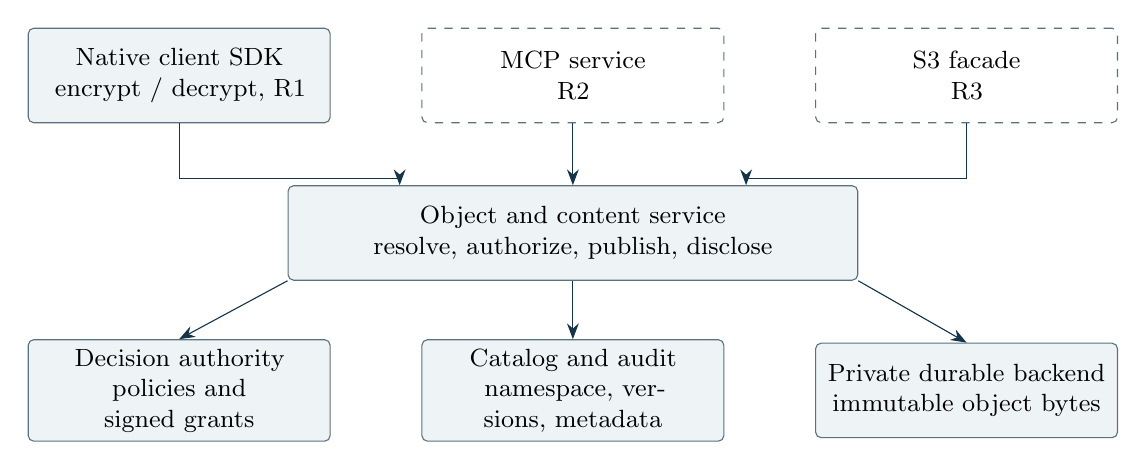
\begin{tikzpicture}[box/.style={draw=ink!70,rounded corners=2pt,fill=pale,align=center,minimum height=12mm,text width=36mm,font=\small},later/.style={box,dashed,fill=white},arr/.style={-{Stealth[length=2mm]},ink}]
\node[box] (http) at (0,0) {Native client SDK\\encrypt / decrypt, R1};
\node[later] (mcp) at (5,0) {MCP service\\R2};
\node[later] (s3) at (10,0) {S3 facade\\R3};
\node[box,text width=70mm] (content) at (5,-2) {Object and content service\\resolve, authorize, publish, disclose};
\node[box] (dec) at (0,-4) {Decision authority\\policies and signed grants};
\node[box] (catalog) at (5,-4) {Catalog and audit\\namespace, versions, metadata};
\node[box] (backend) at (10,-4) {Private durable backend\\immutable object bytes};
\draw[arr] (http.south) -- ++(0,-7mm) -| ([xshift=-22mm]content.north);
\draw[arr] (mcp) -- (content);
\draw[arr] (s3.south) -- ++(0,-7mm) -| ([xshift=22mm]content.north);
\draw[arr] (content.south west) -- (dec.north);
\draw[arr] (content) -- (catalog);
\draw[arr] (content.south east) -- (backend.north);
\end{tikzpicture}
\caption[Storage foundation and later service interfaces]{Object storage and shared access control form the foundation. MCP and S3 communicate with that foundation; they do not introduce another store or authorization system.}
\end{figure}

From R1-B the content service requests only opaque recipient envelopes from the isolated envelope service under signed decisions. Clients verify those envelopes and decrypt locally. Optional model-context assembly and plaintext tools run within authorized client custody; server-side execution has no payload decryptor. These features do not sit on the ordinary object-read or object-write path.
\begin{longtable}{@{}P{0.14\textwidth}P{0.56\textwidth}P{0.14\textwidth}@{}}
\toprule Role & Hosts & First phase\\\midrule\endhead
\code{decision} & Decide/DecideBatch, trusted context, snapshot activation, decision-signing key & R1-A\\
\code{control} & Policy releases, catalog administration and shared approvals; reservation workflows only when the optional executor is enabled & R1-A\\
\code{storage} & Native object/content API, enforcement and publication, external-backend adapter; documents in R1-C & R1-B\\
\code{keys} & Opaque recipient-envelope delivery and registry; no private recipient keys or payload decryptor & R1-B\\
\code{mcp} & Authenticated MCP facade calling content and decision services; no direct backend, client-key or catalog access & R2\\
\code{tools} & Optional encrypted-package or non-content control executor; plaintext model/tool processing belongs to authorized clients & R2, optional\\
\code{blob} & Custom replicated blob service and repair, when selected & R3\\
\bottomrule
\end{longtable}
Roles are deployment and security boundaries of one product, not separate permission domains. The decision service is the only evaluator; no adapter, executor or broker evaluates policy. Storage, decision and catalog availability is qualified before MCP is introduced. Additional MCP replicas cannot bypass storage admission limits or create a second source of permission state.

\subsection{Phase 0 decisions}\label{sec:decisions}
D-01 to D-03 are decided. The others are open: each has a default so that work can be planned, but the default is not a decision until the owner records it. Work gated by an open decision does not start before it is closed.
\begin{longtable}{@{}P{0.06\textwidth}P{0.22\textwidth}P{0.46\textwidth}P{0.12\textwidth}@{}}
\toprule ID & Decision & Options (default first) & Gates\\\midrule\endhead
D-01 & Policy evaluator & Decided: our own evaluator for our own policy format \code{fga.policy/v1} (Section~\ref{sec:policyformat}), in which a matching deny always overrides an allow across roles and scopes. Upstream engines are studied for ideas only (D-03): there is no compatibility promise with any upstream policy format, and no upstream engine is used as a runtime, reference or test oracle. Conditions use CEL through a qualified library. & R1-A\\
D-02 & Object storage & Decided: our own object storage. R1 is a single-node store on local disk behind the backend contract (\rr{BKD-001}), with the catalog in PostgreSQL; the replicated store of Part~5 and the S3-compatible API come in R3. No external object store is used. Everything runs locally for now; the multi-node topology of Section~\ref{sec:availability} is a later target. & R1-B\\
D-03 & Upstream study and license record & Decided in principle: MinIO and Cerbos are studied for ideas only, and no upstream code is copied, translated, paraphrased or reproduced from memory (\rr{SRC-001}). The license record is completed before first distribution (\rr{SRC-004}). & P0\\
D-04 & Identity providers and workload identity & Qualified first-hop authentication and delegation profiles; supported OIDC providers; how workload certificates are issued, rotated and bound to roles (\rr{TRU-002}). & R1-A\\
D-05 & PostgreSQL HA and failure domains & HA controller, quorum-commit and authority-fencing design, failure domains, and the security-state recovery procedure (\rr{AVL-001}, \rr{AVL-008}). & R1-A fence; R1-B recovery; ha profile when deployed\\
D-06 & Label order and label sources & Per-tenant order, authorized labels and collection defaults; which participating client workloads may attest labels or lineage. The server cannot classify encrypted content or verify semantic truth from ciphertext. & R1-C\\
D-07 & First downstream connector & The one real provider used only if the optional external executor is enabled (\rr{SMALL-003}); no connector is required for R1 or baseline MCP. & R2 extension\\
D-08 & Client key custody and recovery & Choose the qualified client SDK, authenticated key-enrollment method, owner or organization custodian and optional client-side hardware/KMS protection. Server recovery has no implicit client-key escrow. Close before any production payload can be uploaded. & R1-B\\
D-09 & Recipient distribution and hierarchy & Flat independent object/unit data keys with client-created recipient HPKE envelopes are the baseline. A document/group KEK is deferred; any later client-only hierarchy requires measured scale benefit, explicit broader compromise scope and separate qualification. The server never unwraps a payload key. & R1-B baseline; later extension\\
D-10 & Limits and S3 client set & Native storage request, object-size, stream and tenant limits close before R1-B. The S3 client list and protocol-specific limits close before R3 (\rr{S3P-005}). & R1-B; R3\\
D-11 & Name and distribution license & Product name, license of original code, license compatibility of dependencies (\rr{SRC-004}). & first release\\
\bottomrule
\end{longtable}

\subsection{Conventions}
Requirements have the form \textbf{[ID]} statement \reqtag{phase}{tests}. Each identifies a coherent behavioral contract and its verification boundary. The phase is one of P0, R1-A, R1-B, R1-C, R2, R3. The tests are identifiers from Section~\ref{sec:testmatrix}; \code{REV} means a release review item and \code{LINT} means the specification check. A superscript \textsuperscript{\color{accent}\tiny NEW} marks a requirement added or strengthened since version 1.3; Appendix~\ref{app:mapping} maps every version 1.3 requirement to its successors.

\must, \mustnot\ and \should\ carry their usual normative meaning. Limits and numbers marked ``initial'' or ``target'' are proposals to be qualified, not measured properties. Sizes use KiB = 1024 bytes. Money uses integer minor units with an explicit currency (\rr{DAT-005}).

The case catalogue and fixtures in \texttt{vectors/} are summarized in Appendix~\ref{app:vectors}. Scenario-only cases state required behavior; concrete fixtures and recorded runs supply qualification evidence (\rr{TEST-003}).

\textbf{Design latitude.} The normative boundaries, authority checks, failure outcomes and release evidence are binding. Interface sketches and module examples explain responsibilities; they do not prescribe incidental names, internal data structures or algorithms. Implementations may choose simpler or better mechanisms that preserve these contracts and demonstrate the same invariants. Byte encodings, dependency pins and operational recipes belong in the qualified companion profiles and runbooks, rather than being inferred from a sketch.

% Expanded source: p01-decision-core

\section{Decision core}\label{sec:decision}
Part~1 defines who is acting, on what, how a decision is made, how it is bound to an operation, and how the authority state is released, stored, audited and kept available. Its business evaluator is independent of payload storage and decryption; the authority service resolves the catalog facts needed to authorize storage operations.

\subsection{Identity and trusted context}
\req{ID-001}{R1-A}{T-03}{Identity comes only from verified OIDC or OAuth tokens, workload certificates, signed S3 credentials, or another explicitly registered authentication provider. Issuer, audience, signature, expiry and intended use are validated.}
\req{ID-002}{R1-A}{T-03}{The platform \mustnot\ accept an agent- or caller-supplied role, tenant, delegation, device state or user identifier as authority.}
\req{ID-003}{R1-A}{T-03}{Adapters submit references and operation facts. The context resolver loads roles, ownership, labels, grants, session limits and approved external signals from authoritative state.}
\req{ID-004}{R1-A}{T-03}{Every trusted context field records its source, observation time, maximum age and revision where available. A missing or stale mandatory envelope fact (verified identity, tenant binding, delegation, version binding) rejects the operation.}
\req{ID-005}{R1-A}{T-03}{External lookups complete before evaluation under a bounded deadline. Policy expressions \mustnot\ fetch data or invoke tools.}
\req{ID-006}{R1-A}{T-03}{Managed-device and recent-authentication facts are usable by policy only when a trusted provider supplies them. A declared purpose may be recorded and constrained but \mustnot\ be inferred as intent. Network origin is trusted only through configured proxies that strip and regenerate forwarding headers.}
\req{ID-007}{R1-A}{T-03}{An ID token \mustnot\ be accepted as an API access token. A JWT access token is accepted only under the resource server's explicit token profile, and opaque tokens only through the provider's supported introspection flow. One JOSE implementation serves all token and envelope signature checks.}

\subsection{Delegation}
The \term{actor} is the executing workload or user. The \term{subject} is the user or service whose authority it exercises. An agent acting for a person carries both; neither inherits the other's full rights.
\req{DLG-001}{R1-A}{T-03}{A delegation record binds actor, subject, audience or executor, resource and action scope, expiry, parent delegation and an optional budget.}
\req{DLG-002}{R1-A}{T-03}{A child delegation can only narrow its parent. Delegation depth is bounded; cycles and unknown parent revisions are rejected.}
\req{DLG-003}{R1-A}{T-01, T-03}{The business-policy principal is the represented subject. Without a delegation the authenticated actor is the principal. Actor and subject role sets \mustnot\ be merged.}
\req{DLG-004}{R1-A}{T-03}{The actor's execution capability and the delegation ceiling are validated independently of business policy. Effective authority is the intersection of actor capability, delegation scope and subject permission.}
\req{DLG-005}{R1-A}{T-03, T-13}{Revocation advances a delegation generation that is checked at admission and at commit.}
\req{DLG-006}{R1-A}{T-03}{A static API key shared by several agents does not identify the user behind each call. A connector using one \mustnot\ claim user-specific enforcement without a verified delegation channel.}
\req{DLG-007}{R1-A}{T-03}{Default credentials carry no implicit administrator or cross-tenant grant. Cross-tenant access requires an explicit, reviewed sharing construct and \mustnot\ result from a missing tenant filter.}

\subsection{Resources, actions and canonical identity}
A \term{check} is one action on one resource binding. A compound operation is several checks evaluated in one batch, all of which must succeed (\rr{RES-006}).
\begin{longtable}{@{}P{0.25\textwidth}P{0.25\textwidth}P{0.31\textwidth}P{0.08\textwidth}@{}}
\toprule Resource type & Example actions & Protected facts & Phase\\\midrule\endhead
\code{storage.bucket} & create-object, list, manage & Retention and encryption requirements, namespace restrictions & R1-B\\
\code{storage.object} & read, stat, discover; read-history, discover-history; new-version, delete, delete-version, share & Tenant, owner, project, label, immutable version, publication state & R1-B\\
\code{document.version} & read-units, raw-read, discover, share, export & Canonical document and version, immutable manifest, full-content coverage & R1-C\\
\code{document.text_unit} & read, share, use-in-model, export-key & Canonical unit and object version, label, lineage & R1-C\\
\code{text.entry} & read, use-in-model, update & Versioned text unit, parent collection & R1-C\\
\code{document.derived} & deliver, declassify, relabel & Lineage, effective label, intended recipient & R1-C\\
\code{crypto.recipient} & enroll, activate, receive-key, revoke & Principal or workload binding, immutable key fingerprint, purpose, status & R1-B\\
\code{crypto.envelope} & create, release, retire & Object, tenant, version, recipient fingerprint, encrypted-envelope digest, status & R1-B\\
\code{platform.policy} & propose, test, approve, activate & Bundle digest, reviewer, tenant scope, activation generation & R1-A\\
\code{storage.replica} & repair, inspect, retire & Blob identity, node incarnation, placement generation & R3\\
\code{agent.tool} & discover, invoke, configure & Registry identity, schema digest, connector, capability class & R2\\
\code{network.destination} & connect, send & Approved hostname or service identity, port, destination class, clearance & R2\\
\code{business.record} & read, update, approve, export & Organization, owner, workflow state, sensitive fields & R2\\
\code{ai.model} & submit, configure & Approved provider and model, endpoint, credential binding & R2\\
\bottomrule
\end{longtable}
\req{RES-001}{R1-A}{T-01, T-06}{Every protected operation maps to one or more (resource, action) checks from the registry. An operation with no registered mapping fails closed.}
\req{RES-002}{R1-A}{T-06}{A canonical resource registry maps native bucket, key and version selectors and, when introduced, S3 selectors, MCP URIs and tool selectors to the same tenant-scoped resource UUID, immutable content version, policy kind, version and scope, and trusted attributes. Role membership and principal context resolve through one identity pipeline.}
\req{RES-003}{R1-A}{T-01, T-06}{Content reading uses the canonical action \code{read}. Legacy route names such as \code{storage.object.read} are aliases, not competing policies. A caller \mustnot\ obtain a less restrictive policy kind or scope by changing protocol.}
\req{RES-004}{R1-A}{T-06}{Alias resolution happens once under a declared catalog snapshot and is bound to the operation. The resource generation is revalidated before admission and publication. ``Latest'' \mustnot\ be resolved again after authorization.}
\req{RES-005}{R1-A}{T-06}{A rename changes a namespace alias, not the resource's permission identity. An edit creates a new immutable version.}
\req{RES-006}{R1-A}{T-06}{A compound operation requires a separate allowed check for every resource and action it actually needs. One allow \mustnot\ authorize an unrelated effect, and \code{tool.invoke} alone \mustnot\ authorize reading the tool's source object or sending to its destination.}
\req{RES-007}{R1-A}{T-01, T-06}{A channel difference affects a decision only through an explicitly declared, trusted context attribute that the policy deliberately uses. Authentication or unsupported-protocol failures stay separate restrictions and \mustnot\ turn a business denial into an allow.}
\req{RES-008}{R1-A}{T-06}{Parent-resource checks configured for a content family apply identically through every transport as explicit compound checks, not as a hidden change to scope inheritance.}

\reqn{RES-009}{R1-B}{T-03, T-11}{Envelope publication uses typed, separately labeled checks for the publishing actor/subject and for the intended recipient principal. The server resolves the target principal, public-key fingerprint, current identity and recipient revisions and read/receive-key eligibility; caller-supplied recipient roles or an untyped principal override are rejected. The signed publication result binds both principal contexts and every required result. During initial upload, prospective recipient eligibility is evaluated against the exact planned LIVE resource state owned by the authorized intent, with its version, labels and digest bound to the commit. This prospective result authorizes only envelope publication, never reading STAGED bytes, user impersonation or a bearer read grant. Commit rechecks the intent, current target revisions and publication preconditions; later sharing checks the current committed state.}

\subsection{Policy evaluation}\label{sec:policy}
\subsubsection{Evaluator contract}
The decision service calls the project's own Go business evaluator, for the project's own policy format (Section~\ref{sec:policyformat}), through a narrow, deterministic contract. Cerbos is studied for ideas only (D-03); neither its implementation, its policy format nor a Cerbos process is used. A qualified CEL library supplies condition evaluation, not policy combination. Decision D-01 is closed.
\begin{lstlisting}
// Logical contract. Pure: no I/O, no ambient state, time passed in.
EvaluatorRequest {
  snapshot_digest,
  policy_set: BUSINESS | CEILING,
  principal: {id, roles, attrs},
  resource:  {kind, id, version, scope, attrs},
  actions:   [string],
  aux:       {envelope facts mapped as documented attributes},
  now
}
EvaluatorResult {
  per_action: [{action, effect, outputs, metadata, diagnostics}],
  // BUSINESS effect: ALLOW or DENY; CEILING effect: PASS or DENY.
  errors:     [{action, kind}]          // strict mode: affected action is DENY
}
\end{lstlisting}
\req{POL-001}{R1-A}{T-01}{Business policy evaluation sits behind the evaluator contract. The conformance corpus (\rr{TEST-003}) qualifies the evaluator. No upstream engine is used as a runtime dependency, reference or test oracle (D-01).}
\req{POL-002}{R1-A}{T-01, T-02}{The evaluator implements the project's own policy format and evaluation rules of Section~\ref{sec:policyformat}. A document or construct that the format does not define is rejected at bundle validation and \mustnot\ be silently ignored.}
\req{POL-003}{R1-A}{T-01}{Evaluation proceeds in this order: (1) authenticate and validate the execution envelope; (2) normalize trusted resource, action and principal input and resolve the scope chain once; (2b) evaluate the ceiling set for every check against that same normalized input, as an always-run gate independent of the business result; (3) evaluate the business set by the rules of Section~\ref{sec:policyformat}, in which a matching deny always overrides an allow; (4) apply the business result unchanged to that check and combine it with the ceiling result so that a ceiling \code{DENY} always wins; (5) fulfil platform prerequisites and obligations. Platform steps add rejections only. They \mustnot\ turn a business denial into an allow.}
\req{POL-004}{R1-A}{T-01}{The response records the business decision and any platform rejection reason separately. A protocol or authentication failure \mustnot\ be reported as a policy-combination rule, and no adapter implements alternate granting logic.}
\req{POL-005}{R1-A}{T-02}{Evaluation is strict. An evaluation error in the condition of any candidate rule for a requested action yields \code{DENY} for that action, or an objection in the ceiling set. The format has no lenient mode and no attribute-schema switch, so no configuration can select one, and a bundle that tries to is rejected at validation.}
\req{POL-006}{R1-A}{T-02}{A missing business attribute is a condition error under \rr{POL-005} and \mustnot\ fall through to an allow. Trusted-envelope facts never depend on business-schema settings: invalid credentials, wrong tenant or resource binding, unavailable authority, malformed transport, process faults and exhausted limits always reject.}
\req{POL-007}{R1-A}{T-01, T-02}{Platform ceilings are a separate, deny-only ceiling set in the signed bundle. Every check is also evaluated against the ceiling set through the evaluator contract (\code{policy_set: CEILING}) before and independently of the business evaluation, and a ceiling \code{DENY} or a ceiling evaluation error denies the check whatever any role or scope result says. The ceiling combiner examines all applicable deny constraints across matching role and scope paths: a matching deny or evaluation error yields DENY; no matching deny, including an explicitly valid empty set, yields PASS. PASS is neutral and never grants an operation; the business result must still be ALLOW. A missing, invalid or stale required ceiling set is not an empty set and rejects. Business no-match remains DENY. Bundle validation rejects a ceiling set that contains an allow rule. A release manifest declares its ceiling set explicitly, and a manifest that omits the declaration is rejected (Section~\ref{sec:policyformat}).}
\req{POL-008}{R1-A}{T-01, T-13}{Time is captured freshly for each request or batch. A time-dependent condition or obligation is supported only when the selected semantic profile can establish a sound next-change bound for all potentially applicable rules. That bound limits decision validity under \rr{DEC-005}; otherwise bundle validation rejects the construct. Admission and commit use current server time with the qualified clock-uncertainty margin, and uncertain clocks fail closed. For \code{fga.policy/v1} the sound bound is the one defined in Section~\ref{sec:policyformat}.}
\req{POL-009}{R1-A}{T-02}{Policy expressions cannot fetch network data, read files, execute scripts or acquire credentials. Compilation, input size, evaluation cost, memory and concurrency are bounded independently of business-policy options.}
\req{POL-010}{R1-A}{T-01}{A snapshot is prepared once per immutable bundle. It contains the validated policy graph, schemas, checked executable expressions, configuration and dispatch indexes keyed by static resource, action, version and scope facts. The index \mustnot\ omit a rule because another path looks permissive. A compiled expression is shared only when the complete environment identity (types, function signatures, schema digests, library and options versions, cost model, evaluator-semantics version) matches.}
\req{POL-011}{R1-A}{T-01}{Policy outputs are data. A mapping from selected output fields to platform obligations is allowed only when explicitly configured, versioned and validated. No mandatory proprietary policy field is introduced for approvals or storage behavior.}
\reqn{POL-012}{R1-A}{T-01}{The conformance corpus of policy-evaluation vectors is part of this specification and runs against the evaluator in CI. No upstream engine is used as a reference or oracle (D-01).}
\req{POL-013}{R1-A}{T-02}{YAML authoring is converted offline into the same strict typed representation as JSON. Ambiguous or unsafe constructs are rejected, and evaluation never runs a YAML parser.}
\reqn{POL-014}{R1-A}{T-01}{Scopes form a dot-separated chain from the request's scope to the root. Rules from every scope on the chain are combined by the same deny-overrides rule, so a child scope can add allows but cannot lift a deny from a parent scope or from the root. No platform guarantee depends on scope inheritance: a guarantee that must hold across tenants is expressed in the ceiling set (\rr{POL-007}) or in a platform gate.}

\subsubsection{Policy format}\label{sec:policyformat}
The policy format is the project's own (D-01) and is identified by \code{fga.policy/v1}. A document holds the rules of one policy set for one resource type in one scope:
\begin{lstlisting}
{
  "format": "fga.policy/v1",
  "set": "business",
  "resource": "document.text_unit",
  "scope": "acme",
  "rules": [
    {"id": "reviewers-read-own-projects",
     "effect": "allow",
     "actions": ["read"],
     "roles": ["reviewer"],
     "when": "resource.attributes.project_id in principal.attributes.project_ids"}
  ]
}
\end{lstlisting}
The ceiling set uses the same document shape with \code{"set": "ceiling"} and deny rules only, for example a rule that denies \code{read} for any role \code{when} the unit is not LIVE.

For one principal, resource and action, the evaluator:
\begin{enumerate}
\item collects the candidate rules of the requested set for the resource type from the request's scope and each ancestor up to the root;
\item treats a rule as matching when it lists the action (or \code{*}), the principal holds one of its roles (or \code{*}), and its condition is true or absent;
\item for the business set, returns \code{DENY} if any matching rule denies, otherwise \code{ALLOW} if any matching rule allows, otherwise \code{DENY};
\item for the ceiling set, reports an objection (\code{DENY}) if any matching rule denies, and \code{PASS} otherwise;
\item denies (or objects) when the condition of any candidate rule fails to evaluate.
\end{enumerate}
An allow rule in the business set may list prerequisites in \code{requires} (\code{approval}, \code{reservation}). An allowed check carries the union of the prerequisites of every matching allow rule, and the decision is \code{NEEDS_APPROVAL} or \code{NEEDS_RESERVATION} until the prerequisite is satisfied through the control plane (\rr{APR-001}, \rr{APR-007}).

Conditions are CEL expressions over \code{principal} (\code{id}, \code{roles}, \code{attributes}), \code{resource} (\code{type}, \code{id}, \code{scope}, \code{attributes}) and \code{request} (\code{now}, and the operation facts supplied by the registered operation, never by the caller as authority; \rr{ID-003}). They are compiled once per bundle and run under a cost limit. Because a deny always overrides an allow, holding an extra role cannot undo a deny (vector V-005), and no business rule can bypass a ceiling. Principal-specific policies, derived roles, shared variables and outputs are not part of version 1; they can be added later without changing the meaning of existing policies.

\textbf{Ceiling declaration.} A release manifest (\rr{REL-001}) names its ceiling set explicitly. A manifest with no ceiling documents is valid only when it declares the ceiling set empty, in which case every check passes the ceiling gate. A manifest that omits the declaration is rejected, so a missing ceiling set is never mistaken for an empty one (\rr{POL-007}).

\textbf{Time conditions.} \code{request.now} may appear in a condition only as one side of a direct comparison with a timestamp literal; any other use, such as arithmetic on \code{request.now} or a comparison with an attribute, is rejected at bundle validation because no sound next-change bound exists for it. The \code{valid_until} of a decision is then bounded by the earliest timestamp literal later than the request time among the conditions of all rules of both sets that list the requested action for the resource type and scope chain, whether or not they matched (\rr{POL-008}, \rr{DEC-005}).

\subsubsection{Platform ceilings and scopes}
A tenant scope is a policy selector, not proof of tenant identity (tenant binding is a platform gate). Scopes form a chain from the request's scope to the root, and the rules of every scope on it combine by deny-overrides (\rr{POL-014}): a child scope can add allows but cannot lift a deny of its parent or of the root. Platform ceilings therefore live in a separate deny-only set that is evaluated for every check (\rr{POL-007}), so no business rule, principal attribute or scope can bypass them.
\begin{lstlisting}
{"format": "fga.policy/v1", "set": "ceiling", "resource": "document.text_unit", "scope": "",
 "rules": [{"id": "only-live-units", "effect": "deny", "actions": ["read", "use-in-model"],
            "roles": ["*"], "when": "resource.attributes.state != \"LIVE\""}]}

{"format": "fga.policy/v1", "set": "business", "resource": "document.text_unit", "scope": "acme",
 "rules": [{"id": "reviewers-read-own-projects", "effect": "allow", "actions": ["read"],
            "roles": ["reviewer"],
            "when": "resource.attributes.project_id in principal.attributes.project_ids"}]}
\end{lstlisting}
If one role's rule denies \code{read} and another role's rule allows it, the result for a principal holding both roles is \code{DENY}.

\subsection{Decision API}\label{sec:decisionapi}
\begin{lstlisting}
DecideBatch request {
  request_id, tenant_id, adapter_id, operation_id,
  actor:      {id, type, identity_revision},
  subject:    {id, type, identity_revision},
  delegation: {id, revision},
  session:    {id, binding_revision, context_key,
               mark_revision, label_order_generation},
  checks:     [{check_id, action, check_kind, principal_binding,
                resource: {type, id, version, generation, metadata_revision}}],
  operation_digest, required_policy_epoch, deadline
}
DecisionResponse {
  outcome: ALLOW | DENY | NEEDS_APPROVAL | NEEDS_RESERVATION | ERROR,
  reason_code, decision_id,
  policy_results: [{check_id, principal_id, resource_id, action,
                    business_effect | NOT_EVALUATED,
                    ceiling_effect: PASS | DENY | NOT_EVALUATED,
                    policy_outputs,
                    policy_metadata, diagnostics}],
  bundle_digest, policy_epoch, evaluator_version,
  actor_id, subject_id, delegation_revision,
  operation_digest, resource_bindings_digest, context_revisions,
  evaluated_at, valid_until, recovery_incarnation,
  obligation_mapping_version, obligations_digest,
  obligations: [{type, version, parameters_or_ref, parameters_digest,
                  referenced_record_revisions}],
  session_mark_revision_after,        // only for the optional mediated profile
  signature                       // detached JWS, see DEC-008
}
\end{lstlisting}
The wire schema distinguishes an ordinary authenticated storage request from a delegated or mediated-context request. Session, context-mark and label-order fields are present only when their registered operation/profile requires them; an ordinary storage client needs no agent session. Missing facts required by the selected profile reject rather than silently selecting a weaker profile.

\code{Decide} is a batch of one. A platform-gate rejection returns \code{DENY} with a platform reason code and \code{NOT_EVALUATED} business effects. \code{ERROR} means the service could not decide (timeout, unavailable authority, resource limit).
\textbf{Check kinds.} Each check names how its principal is determined. An \code{OPERATION} check is evaluated for the request principal: the represented subject, or the authenticated actor acting for itself (\rr{DLG-003}); its \code{principal_binding} is empty. A \code{RECIPIENT_ELIGIBILITY} check (\rr{RES-009}) is evaluated for the intended recipient: its \code{principal_binding} carries the recipient's public-key fingerprint, the decision service resolves it to a principal, key version and identity revision from authoritative state, and the response records the resolved \code{principal_id} for that check. A caller cannot supply recipient roles or attributes, and an unresolvable or revoked fingerprint denies the batch. The checks of one batch share one policy snapshot and one authority envelope but may differ in principal (\rr{DEC-004}).

\req{DEC-001}{R1-A}{T-01}{The decision API is exposed as versioned gRPC for internal services and an authenticated JSON facade for SDKs with the visibility boundary of \rr{DEC-010}. The caller \mustnot\ choose an action mapping different from the registered operation.}
\req{DEC-002}{R1-A}{T-01}{The enforcement point acts only on an explicit, complete \code{ALLOW} bound to its exact operation. \code{DENY}, \code{NEEDS_APPROVAL}, \code{NEEDS_RESERVATION}, \code{ERROR}, transport errors, malformed data, unknown required obligations and missing results all stop execution. A prerequisite outcome is satisfied through the control plane, after which a new \code{ALLOW} whose context revisions include the approval or reservation is required.}
\req{DEC-003}{R1-A}{T-01}{Each internal enforcement response carries the per-check business and ceiling effects, outputs, metadata, redacted diagnostics, bundle digest, policy epoch, evaluator version, identity and delegation revisions, operation and resource-bindings digests, validity and obligations. A platform gate that stops evaluation is reported with an explicit not-evaluated marker and \mustnot\ authorize execution.}
\req{DEC-004}{R1-A}{T-01}{A batch captures one policy snapshot and one authority envelope. Items have unique identifiers and exact resource, action and revision bindings. A missing, duplicated or misbound result \mustnot\ authorize its operation, and a failed item \mustnot\ grant its peers. A batch is an evaluation optimization, not a transaction over writes or external effects.}
\req{DEC-005}{R1-A}{T-13}{\code{valid_until} is bounded by the earliest of identity or session expiry, delegation expiry, approval or grant expiry, context freshness limit, request deadline, decision-age limit and the next possible change of any applicable temporal policy condition or obligation (\rr{POL-008}). Validity is half-open: admission at or after that time rejects or obtains a fresh decision. A decision is not a general bearer permission.}
\req{DEC-006}{R1-A}{T-13}{At read or delivery admission and at a mutation or egress checkpoint, the enforcing service verifies the exact evaluated operation, expiry, recovery incarnation and every bound authority revision: identity, delegation, resource generation, metadata, parent/unit access and labels, recipient/envelope state, policy epoch and, where applicable, lineage dependencies, context mark and label-order generation. These checks and the protected catalog transition or durable admission share the serialization fence of \rr{DAT-007}; an intervening authority change cannot pass unnoticed. A mismatch requires a new decision or rejection.}
\req{DEC-007}{R1-A}{T-03}{Identity and capability checks are enforced at the decision API itself. mTLS workload identity or an equivalent bound credential identifies the adapter, not the user it names. The decision service verifies that user's authentication or delegation evidence under \rr{TRU-003}; neither an adapter nor an ordinary user can supply fabricated verified context.}
\reqn{DEC-008}{R1-A}{T-03}{The authority signs every retained or cross-process \code{ALLOW} with its dedicated decision-signing key. The versioned strict wire profile authenticates the exact transmitted bytes and binds decision ID; audience (deployment, role and service); tenant and recovery incarnation; actor, subject, delegation and context with revisions; operation and resource bindings; every check and effect; bundle digest and epoch; all freshness dependencies; issue time and \code{valid_until}; and the complete obligation set, its mapping version, parameter values or digests, and referenced-record revisions. Missing, added or altered obligations reject. Protobuf alone is not a canonical encoding: schemas, parsing rules, signing profile and interoperability bytes are frozen before qualification. Verifiers check signature, audience, expiry, replay and \rr{DEC-006}; signatures do not establish user intent or replace fresh authority.}
\req{DEC-009}{R1-A}{T-22}{Initial qualification limits are a 250 ms single-decision budget, 64 KiB of context, 50 resources per batch, 8 KiB of expression text, bounded AST depth, 10,000 expression cost units per condition and a total request budget. These are proposed limits, not measured guarantees; independent input, compilation, allocation, concurrency and cancellation limits are mandatory, and cancellation reaches both queued and running evaluation.}
\req{DEC-010}{R1-A}{T-01}{The public decision facade applies the same existence and metadata visibility rules as the content API. Outcomes, reason codes, policy outputs, metadata, diagnostics and obligation parameters are projected to facts the caller is authorized to observe; an absent target and an undiscoverable denied target receive the same public denial representation. Dependency failures may remain distinguishable without revealing target-specific facts. Complete signed enforcement responses and obligations remain available to their authorized enforcement audience; a public projection cannot authorize execution.}
\reqn{DEC-011}{R1-A}{T-03}{Single-use decision consumption for a mutation or encrypted-envelope delivery is an atomic, durably acknowledged catalog compare-and-set shared by every verifying replica. It commits with the protected transition or exact delivery admission under \rr{DAT-007}, before the effect begins. Unavailable consumption state rejects; a recovery-incarnation mismatch rejects even if an old consumption record was lost. Durability waits do not extend decision validity: expiry before first emission or dispatch requires fresh authority, while the old single-use decision remains consumed.}
\reqn{DEC-012}{R1-A}{T-03}{Decision-signing keys are distinct from workload, issuer and encryption keys. Key identifiers reach verifiers through the control plane, rotation uses an overlap window no shorter than the longest \code{valid_until} plus clock skew, and a compromised signing key is revoked by a revision that verifiers must observe before accepting further decisions. Rotation and revocation are qualified under T-03.}

\subsection{Policy releases and readiness}
\req{REL-001}{R1-A}{T-14}{A policy release is an immutable, signed bundle whose manifest includes schema and evaluator versions, source hashes, the business set, the ceiling set, the label order and its generation, resource schemas, operation registry, pure-function allowlist, expression-library version and cost model, test evidence, target audience and digest. Each instance verifies, parses, compiles, validates and checks a candidate into an immutable in-memory snapshot before atomically replacing its active pointer. A failed activation preserves the prior valid state and does not acknowledge the candidate.}
\req{REL-002}{R1-A}{T-14}{Activation records the states RECEIVED, VERIFIED, PREPARED, READY, ACTIVE or REJECTED with digest, environment version, preparation error and timestamps. Every decision uses exactly one snapshot, and preparation and old-snapshot coexistence are resource-bounded.}
\req{REL-003}{R1-A}{T-13, T-14}{A node that cannot establish the authoritative required epoch \mustnot\ authorize new operations. The last valid snapshot is kept only while it satisfies that epoch. Offline authorization is not an availability fallback.}
\req{REL-004}{R1-A}{T-14}{The control plane stages a candidate pool, verifies sentinel allow and deny cases, records ready instances by digest, advances the durable tenant-required epoch under \rr{DAT-007}, and routes only to compatible instances. A restrictive activation may stop admissions and drain bounded mutation leases. A rollback is a new reviewed release with a higher epoch, because silently reverting may restore revoked access.}
\reqn{REL-005}{R1-A}{T-14}{Before activation the candidate is run over the conformance corpus and the tenant's sentinel cases, and the change in effect against the active release is reported to the reviewer, who must acknowledge it. The report covers the corpus and sentinels only; it does not enumerate every principal.}
\req{REL-006}{R1-A}{T-14, T-19}{Liveness reports process progress and does not restart a healthy process because PostgreSQL, the private backend or a peer is unavailable. Readiness is role- and capability-specific (policy digest and epoch, catalog authority, workload credential validity, recipient-envelope state and enabled connector dependencies). Probes return redacted aggregate state, are rate-limited, and never create a key or expose protected content. A readiness result is never a grant; requests perform their own admission checks.}

\subsection{State and catalog}
PostgreSQL holds authoritative identities, grants, resource bindings, revisions, approvals, reservations and audit-outbox records.
\begin{longtable}{@{}P{0.20\textwidth}P{0.62\textwidth}P{0.08\textwidth}@{}}
\toprule Entity & Minimum authoritative fields & Phase\\\midrule\endhead
Principal, delegation & Stable IDs; tenant; actor and subject bindings; credential class; roles; limits; expiry; revocation and identity revisions & R1-A\\
Resource & UUID; type; tenant; protected attributes; metadata revision; resource generation; lifecycle state & R1-A\\
Authority recovery & Current recovery incarnation and admission state; restore reconciliation evidence from R1-B & R1-A\\
Policy release & Canonical manifest digest; schema, configuration, evaluator and expression-library versions; tests; publisher signature; activation epoch & R1-A\\
Audit outbox & Unique event ID; decision and operation IDs; redacted bindings; outcome; delivery status & R1-A\\
Tool registry & Stable tool ID; schema digest; connector version; operation mapper; allowed destinations; required capabilities; credential binding & R2\\
Invocation & Tenant and idempotency unique key; argument digest; state; dispatch attempt and fencing token; downstream receipt; reconciliation status & R2\\
Approval & Exact operation digest; approver; subject and actor; resource revisions; expiry; allowed uses; consumption state & R1-B\\
Reservation & Budget or grant ID; minor-unit amount or use count; invocation ID; status; lease; reconciliation state & R2\\
Object, version & Bucket and exact key; stable object UUID; current committed version; content generation; immutable blob ID; length and checksums & R1-B\\
Document manifest, text unit & Document and version UUIDs; ordered unit IDs; manifest digest; extraction and normalization version; unit order; labels; access revision; provenance & R1-C\\
Upload intent & Operation and idempotency IDs; principal and delegation; expected generation and current version; intended labels; staged blob; state; expiry & R1-B\\
Context mark & Context key (runtime context ID, else delegation ID); bound actor, subject and delegation; label-order generation; highest effective label; mark revision & R2\\
Recipient key, key envelope & Tenant; principal or workload; immutable key ID and fingerprint; purpose and suite; activation and revocation revision; opaque recipient-encrypted key envelope; sender signature; generation; status & R1-B\\
Maintenance job & Kind; tenant and blob scope; expected placement generation; idempotency key; lease and fence; progress; initiating actor & R3\\
\bottomrule
\end{longtable}
\req{DAT-001}{R1-A}{T-01}{All authoritative lookups include tenant scope. Tenant-consistent references are enforced with database constraints or equivalent transaction checks. Tenant isolation \mustnot\ depend on policy authors writing a tenant condition.}
\req{DAT-002}{R1-A}{T-03}{Protected fields change only through explicit authorized control operations with expected revisions. Raw S3 tags, tool arguments and external payloads \mustnot\ become trusted ownership or classification records.}
\req{DAT-003}{R1-A}{T-06, T-13}{Resource metadata revision and content or resource generation are distinct. Every logical publication, deletion or target-state mutation increments the generation, and approval and execution comparisons include state changes even when access labels have not changed.}
\req{DAT-004}{R1-A}{T-13, T-14}{Permission-critical facts use authoritative consistent reads. The first release has no allow-result cache. A cache, if added, requires a maximum age, revision-aware keys and explicit invalidation. A decision uses one immutable policy snapshot and one declared context snapshot. Search indexes and storage notifications are discovery aids, not access authority.}
\req{DAT-005}{R2}{T-05}{Money uses integer minor units with an explicit currency. Binary floating point \mustnot\ be used for permission thresholds or budget consumption.}

\reqn{DAT-006}{R1-B}{T-18, T-19}{Catalog, policy bundles, audit persistence, indexes, temporary files and backups use qualified encryption at rest and access-separated credentials. Payload confidentiality uses the client-encrypted format of Part~4 in addition to backend encryption. The server may read only the minimum authorization and routing metadata declared in the schema; sensitive titles, document text, prompts and content-derived fields are encrypted by clients. Fields hidden from the server cannot be used as server-evaluated policy attributes or search predicates. No metadata or logging path is an implicit plaintext payload channel.}

\reqn{DAT-007}{R1-A}{T-03, T-13, T-14}{Final authority checks and their catalog transition or durable admission have one atomic ordering point shared with every change to the facts checked, including revocation and policy activation. If the authority change wins that ordering, a stale operation cannot commit or enter delivery; if admission wins, only that exact admitted operation and its bounded lease may proceed. Snapshot reads alone do not establish this fence~\cite{postgresIsolation}. The implementation records and qualifies its locking, transactional or equivalent fencing protocol; policy evaluation and external calls stay outside held database locks.}

\subsubsection{Authorization facts and storage decisions}
The implementation separates three kinds of data. Verified identity, membership and delegation come from the identity/control authority. Object ownership, tenant, policy scope, publication state and access revisions come from the catalog and explicit protected-metadata operations. Caller-supplied selectors, proposed labels, destinations and expected versions are request facts only until the registered operation validates them. Encrypting a document does not make its uploader's claims about ownership, classification or lineage true.

An object read therefore follows one path: authenticate; resolve the tenant-scoped alias and immutable version; load its protected facts and applicable parent checks; evaluate platform ceilings and business policy; bind every result to the exact operation and recipient; then recheck authority at admission. A usable download package also needs the encrypted-envelope conjunction in Table~\ref{tab:keyops}. A write additionally checks the bucket's creation authority or the object's new-version authority and repeats current checks at publication. Granting access to ciphertext does not create a missing recipient envelope or let the server manufacture a decryption key.

New tenants, buckets, objects, versions, recipients and routes have no implicit public or administrator access. No matching allow, missing policy, failed schema validation, absent mandatory fact, unknown obligation, unavailable authority or failed recipient binding stops the operation (\rr{DEC-002}, \rr{POL-005}, \rr{POL-006}). Configuration never turns an error into public access. An explicit business allow remains bounded by tenant isolation, delegation, platform ceilings and operation-specific prerequisites.

The native evaluator owns format decoding, scope-chain combination, policy outputs and strict error handling. CEL owns bounded expression execution only. Bundles compile offline into immutable snapshots; each request selects exactly one required epoch. Preparation indexes static selectors and preserves every potentially applicable deny rule. No policy expression performs I/O, and no storage or MCP component repeats the combination logic (\rr{POL-009}, \rr{POL-010}).

\subsection{Audit}
\req{AUD-001}{R1-A}{T-15}{Decisions and actual outcomes are logged separately and joined by decision, operation and invocation IDs. Records include actor, subject, tenant, action, resource, version and generation, relevant context provenance, policy digest and epoch, reason, latency and redacted obligations. External tools record dispatch and receipt or reconciliation evidence.}
\req{AUD-002}{R1-A}{T-15}{Attempt, decision, encrypted-envelope delivery, durable mutation, approval consumption and external delivery are distinct events. Mandatory records are appended transactionally to an outbox and \mustnot\ silently disappear when the exporter is disabled or a queue is full; capacity alarms and declared admission limits act before required evidence can no longer be recorded. Operational logs and optional notifications are not a substitute for the outbox.}
\req{AUD-003}{R1-A}{T-19}{Audit delivery is idempotent with explicit retention and access policies. Sensitive labels and arguments are minimized or protected, lag, loss, stale policy nodes, failed context resolution and revocation latency are monitored, and metrics \mustnot\ create a cross-tenant information channel.}
\req{AUD-004}{R1-A}{REV}{An envelope-delivery audit record proves that encrypted material was issued, not that a user opened plaintext or complied with a purpose restriction. Documentation \mustnot\ present it as proof of use.}

\subsection{Administration}
\req{ADM-001}{R1-A}{T-20}{Policy authors, reviewers, activators, key administrators, storage operators and data users are separate roles. A policy administrator is not automatically a data reader, and sensitive policy or key changes use the approval and reservation model where configured.}
\req{ADM-002}{R1-A}{T-20}{An ordinary API request \mustnot\ disable the authorizer, change trusted issuers, relax workload audience checks, replace trusted recipient or signing-key bindings or grant itself policy-administrator authority. Those changes use explicit administrative actions and reviewed control transactions.}
\req{ADM-003}{R1-A}{REV}{Bootstrap and recovery authority sits outside ordinary agent paths, with controlled local or separately authenticated recovery and a durable incident audit. Recovery procedures \mustnot\ claim to defend against a host operator who can replace the running software.}

\subsection{Availability of authority state}\label{sec:availability}
This section covers R1 storage, decision, control, encrypted-envelope delivery and catalog availability. Optional R2 workers join only when their service is enabled. The private byte backend must be qualified for the selected failure domains; custom blob replication is in Part~5. Two deployment profiles exist. The \code{local} profile (D-02) runs every role on one host with a single PostgreSQL instance and our own single-node blob store; it is the R1 target. The \code{ha} profile is the multi-node topology of the table below and is qualified only when it is deployed. Under \code{local} the obligations that apply are those of AVL-003 (database durability settings), AVL-006, AVL-008 and the backup, restore and client-key-recovery parts of AVL-005; no zero-loss claim is made, and losing the node loses blobs and catalog changes written since the last backup. AVL-001, AVL-002, the standby conditions of AVL-004 and AVL-007 apply to \code{ha}.
\begin{longtable}{@{}P{0.20\textwidth}P{0.40\textwidth}P{0.30\textwidth}@{}}
\toprule Layer & Initial production topology & Failure contract\\\midrule\endhead
Storage, decision, control, envelope service & At least 3 stateless replicas across 3 failure domains, required bundle digest on each & Load balancer removes unready replicas; stale or unavailable authority never becomes allow\\
Optional R2 executors & At least 3 workers sharing durable invocation state when enabled & Leases and fencing plus downstream idempotency; no blind redispatch after timeout\\
Catalog PostgreSQL & Primary plus 2 standbys; commit durable on the primary and at least one synchronized remote standby (quorum commit) & HA coordinator promotes only a safe candidate and fences the old primary; no silent asynchronous downgrade\\
\bottomrule
\end{longtable}
\req{AVL-001}{R1-B}{T-15, T-16}{The \code{ha} profile runs the topology above and rejects a single-node configuration. The \code{local} profile is the single-node R1 profile (D-02). A configuration declares exactly one profile, and a node that declares \code{ha} without the required replicas, standbys and failure domains refuses to become ready.}
\req{AVL-002}{R1-B}{T-16}{Authorization-critical reads use the primary or a standby proven sufficiently fresh by a log-position check. An arbitrarily lagging standby \mustnot\ restore revoked grants.}
\req{AVL-003}{R1-B}{T-16}{PostgreSQL runs with \code{fsync=on}, \code{full_page_writes=on}, \code{synchronous_commit=on} or stronger, and, in the \code{ha} profile, a non-empty synchronous standby set; \code{remote_write} alone is insufficient against an operating-system crash. With Patroni, strict synchronous mode is enabled. Failover uses a managed HA service or established controller with quorum coordination and old-primary fencing, and promoting an unqualified stale replica voids the zero-loss objective.}
\req{AVL-004}{R1-B}{T-16}{A timeout or cancellation while awaiting synchronous commit has an unknown outcome; visibility of an operation row is not durability evidence. Before durable success, external dispatch or envelope emission, establish that the required standby set flushed the original commit on the current fenced timeline. A later-commit barrier must generate WAL, be ordered after that commit and receive synchronous acknowledgement; a read-only transaction is insufficient~\cite{postgresHA}. Direct flush-position evidence must establish timeline ancestry as well as position. The chosen barrier is qualified across cancellation, reconnection, standby changes and failover; until then the result remains unknown. In the \code{local} profile the local WAL flush of the commit is the evidence, and an uncertain commit is reconciled by operation identity.}
\req{AVL-005}{R1-B}{T-15, T-18}{For the \code{ha} profile the design target is zero loss of acknowledged operations under the loss of one failure domain in a crash-fault model, conditional on synchronous database acknowledgement, correct fencing and recoverable client key state; it is not a guarantee against simultaneous multi-domain loss, Byzantine replicas, malicious deletion or untested hardware. Recovery of the target service within five minutes is an acceptance objective, not a benchmark. Encrypted, access-separated backups of the catalog, policy bundles and opaque recipient-key envelopes are restored together in tests. Client private-key recovery is separately owned and qualified by the client or organization; server backups contain no payload keys or client private keys, and replication is not a substitute for backups.}
\req{AVL-006}{R1-B}{T-22}{Tenant-aware admission limits cover requests, bytes, active streams, expression cost, scan candidates, client-envelope delivery and, when enabled, reservations and external-tool concurrency. Client crypto cost and server envelope throughput are measured separately. Overload uses backpressure and bounded queues rather than unbounded goroutines, and retries use jitter and budgets. Circuit breakers reject rather than grant.}
\req{AVL-007}{R1-B}{T-22}{The first metadata authority is one PostgreSQL primary (with HA in the \code{ha} profile). When measured write capacity is exceeded, tenants are sharded across independent catalog groups with an explicit tenant-to-shard registry and migration fencing, and cross-shard grants and budgets are not treated as local atomic operations. The first region is active for each tenant; multi-region active-active authorization requires a later consistency design.}

\reqn{AVL-008}{R1-B}{T-13, T-16, T-18}{Backup restore starts with admission closed. Before reopening, recovery reconciles security-critical authority changes after the backup, including revocations, restrictive policy releases and signing/recipient-key status, from a separately protected recovery record or re-established current authority. It issues a fresh recovery incarnation that invalidates old decisions, sessions and continuation tokens. An incarnation change cannot recover lost revocations: if current authority cannot be established, affected access remains closed pending explicit reauthorization. A data-recovery RPO is not permission to silently restore old grants. Test backup, revocation, restore and attempted new envelope delivery.}

% Expanded source: p02-enforcement

\section{Storage enforcement and service adapters}\label{sec:enforcement}
Part~2 starts with the enforcement contract used by the native object API and the shared storage service. R1 binds authorization to actual object and document operations, including publication, read admission, metadata changes and deletion. R2 adds MCP as a separate service that calls those established APIs. External tool execution, model submission and execution-context flow control are optional services built on the same foundation; they do not define the storage product or gate its first release. Part~3 defines the shared content operations consumed by every interface.

\subsection{Shared adapter contract (R1-B)}
The native object API is the first adapter. Its prepared plans identify canonical objects, versions, actions and preconditions; execution enters the shared content service rather than a tool executor. The same contract later applies to MCP and S3.
\begin{lstlisting}
// Logical design; generated DTOs are defined by the versioned API.
type EnforcementAdapter interface {
    Prepare(ctx context.Context, request AdapterRequest) (OperationPlan, error)
    Execute(ctx context.Context, plan OperationPlan, grant Grant) (Outcome, error)
}

type OperationPlan struct {
    ID              string
    RegistryVersion string
    RequiredChecks  []Check
    ArgumentsDigest string
    ResourceBindings []ResourceBinding
    IdempotencyKey  string
}
\end{lstlisting}
\req{ENF-001}{R1-B}{T-04}{Every adapter implements \code{Prepare} and \code{Execute}. \code{Prepare} resolves targets and validates arguments without performing the protected side effect. \code{Execute} verifies the grant, carries out the required obligations and dispatches only the prepared plan.}
\req{ENF-002}{R1-B}{T-04}{An adapter request is a validated typed protocol or domain variant. It \mustnot\ be an unrestricted \code{any} or an arbitrary attribute map, and each concrete adapter accepts only its declared request kind.}
\req{ENF-003}{R1-B}{T-01, T-04}{An adapter translates authentication evidence, selectors, operation parameters and response framing. It \mustnot\ fork business grants, duplicate policy combination, invent its own context format, turn an unknown policy result into a local allow, or perform a permissive check and then bypass the shared service.}
\req{ENF-004}{R1-B}{T-04}{Where target resolution is itself sensitive, it requires a separate discovery or stat action.}
\req{ENF-005}{R1-B}{T-04}{Every adapter declares its discovery, read, mutation, output-transformation, batching, streaming and obligation capabilities. An unknown capability fails closed. Public API clients receive redacted errors while internal audit retains diagnostic detail, and the resource-to-action mapping is versioned with policy and schema releases.}
\req{ENF-006}{R1-C}{REV}{Database row or column filtering, filesystem mounts, message consumption and job scheduling are extension points that need real enforcement at their own access boundary. The first release does not compile expressions into SQL; a later optimizer must translate a declared subset, prove equivalence against per-resource decisions and never drop an unsupported predicate. A database adapter exposes a field only if it actually builds a restricted query or response.}

\subsection{Trust propagation}\label{sec:trust}
Authentication at an ingress is insufficient if a downstream service can be reached another way. Each internal call carries the evidence in Table~\ref{tab:hops}, and the receiver rejects a call that lacks it.
\begin{longtable}{@{}P{0.06\textwidth}P{0.20\textwidth}P{0.46\textwidth}P{0.10\textwidth}@{}}
\caption{Evidence that crosses each boundary}\label{tab:hops}\\
\toprule TB & Hop & Evidence the receiver verifies & Phase\\\midrule\endfirsthead
\toprule TB & Hop & Evidence the receiver verifies & Phase\\\midrule\endhead
TB1 & Client \arrowto\ native object API & Token or credential for this audience, verified actor and subject, and delegation when acting on behalf of another principal (\rr{ID-001}, \rr{TRU-003}); no MCP session is required & R1-B\\
TB2 & Adapter \arrowto\ decision & Adapter-role credential plus independently verifiable user authentication evidence or an authoritative delegation binding (\rr{TRU-003}); references, not asserted facts (\rr{ID-003}) & R1-A\\
TB2 & Decision \arrowto\ adapter & Signed decision for this audience, operation and validity (\rr{DEC-008}) & R1-A\\
TB3 & MCP service \arrowto\ content service & Workload certificate of the \code{mcp} role, plus signed decision or a delegation reference verified against authoritative state (\rr{TRU-003}); the storage service performs the same final checks as for native clients & R2\\
TB3 & Content service \arrowto\ envelope service & Workload certificate of the \code{storage} role plus a signed decision whose checks are exactly those of the matching operation mapping of Table~\ref{tab:keyops}, bound to the exact object, version, unit and recipient (\rr{TRU-005}) & R1-B\\
TB4 & Optional executor \arrowto\ connector & Target-specific restricted credential, never the model's credential (\rr{AGT-006}) & R2\\
TB4 & Optional executor \arrowto\ downstream & Idempotency key and state precondition where supported (\rr{AGT-006}, \rr{INV-005}) & R2\\
TB5 & Storage \arrowto\ blob backend & Backend-scoped workload credential on every call; only storage and authorized maintenance workloads have backend access (\rr{BKD-001}) & R1-B\\
\bottomrule
\end{longtable}
\req{TRU-001}{R1-A}{T-03}{Each cross-process hop carries the evidence listed in Table~\ref{tab:hops}. A receiver that does not find it rejects the call.}
\req{TRU-002}{R1-A}{T-03, T-20}{Workload identity uses mTLS or an equivalent bound credential issued by the workload certificate authority chosen in decision D-04, bound to one role. Certificate verification is mandatory configuration, not an optional check.}
\reqn{TRU-003}{R1-A}{T-03}{To obtain the first decision, an adapter carries independently verifiable evidence of user authentication by a registered provider, or a delegation reference verified against authoritative state. The receiver validates the evidence for its intended audience and binds it to the presented actor and subject; D-04 records the qualified authentication and delegation profiles. This needs no prior decision or agent session and grants no operation by itself. Subsequent enforcement hops carry a signed decision (\rr{DEC-008}) or a verified delegation reference as specified in Table~\ref{tab:hops}. Caller-asserted identity claims plus a workload identity are never sufficient.}
\reqn{TRU-004}{R1-A}{T-03}{A role accepts only signed decisions whose audience is that role, and the decision-signing key is registered separately from workload, issuer and encryption keys.}
\reqn{TRU-005}{R1-B}{T-11}{The envelope service delivers an opaque recipient-encrypted key envelope only against a signed decision whose checks are exactly those of the matching operation mapping in Table~\ref{tab:keyops} and that is bound to the exact object, version, unit and recipient being released. The service verifies the complete signed result, not a subset, whether or not the request also carries an mTLS identity. No server role can unwrap the envelope or obtain a plaintext data key. The authenticated recipient fingerprint is fixed by the client-origin envelope; a gateway cannot substitute its own key.}
\req{TRU-006}{R2}{T-03}{The MCP adapter calls the same content-service implementation as every other adapter and preserves the represented principal and delegation. It \mustnot\ replace the user with a broadly privileged connector account.}

\subsection{Native HTTP and service API (R1-B)}
\req{ADP-001}{R1-B}{T-06}{HTTP middleware authenticates the caller, resolves the route and resource, validates the request body and checks the exact semantic action immediately before protected work. Path parameters and request bodies are not authoritative ownership records.}

\subsection{Storage approvals and later reservations}
R1 supports operation-bound approvals where a storage policy requires them, such as protected metadata changes or destructive operations. Approval consumption uses the same catalog transaction or durable execution checkpoint as the protected operation. It does not require the external tool invocation engine. R2 adds budget reservations for optional external effects. A release that cannot enforce a requested obligation denies the operation rather than ignoring the obligation.
\req{APR-001}{R1-B}{T-04}{A prerequisite approval or reservation is satisfied before execution. An approval binds the exact operation digest, actor and subject, target, relevant resource revisions, policy epoch, expiry and permitted uses, and a change to any material fact invalidates it.}
\req{APR-002}{R1-B}{T-05}{Approver authority and the prohibition on self-approval are checked separately. Approval consumption is atomic with the protected operation's catalog transition or durably recorded execution admission. Where R2 reservations apply, they are consumed in the same transaction. A caller- or model-generated assertion \mustnot\ stand in for the approval record.}
\req{APR-003}{R1-B}{T-05}{An approval is consumed at the documented execution checkpoint, not when it is merely displayed.}
\req{APR-004}{R2}{T-05}{A reservation cannot exceed its parent grant or budget under concurrency. Capacity is reserved under row-level locking or serializable transactions with unique operation and idempotency keys.}
\reqn{APR-005}{R1-B}{T-04}{The summary shown to an approver is rendered by the platform from the canonical operation plan: action, exact object or document versions, relevant metadata changes and preconditions; tool, amount, destination and highest source label are included when applicable. Agent- or model-supplied descriptions may be displayed only as clearly labeled unverified notes.}
\req{APR-006}{R2}{T-05}{Cancellation, expiry, outcome-unknown and compensation are distinct states.}
\req{APR-007}{R1-B}{T-04}{Obligations from several sources merge restrictively: field and destination sets intersect, required projections intersect, and limits take the minimum. The complete merged set and mapping version are authenticated by \rr{DEC-008}; enforcement never substitutes unsigned values. Conflicting or unsupported obligations reject before their effect or disclosure. Server inspection or redaction of encrypted payload is unsupported; select independently encrypted units instead.}

\subsection{Shared classification order (R1-C)}
\reqn{FLW-004}{R1-C}{T-21}{Labels form a tenant-defined total order in the signed bundle, identified by an order generation, and the order is immutable within a generation. A unit or output with no label counts as the highest level. In the R2 flow-control profile, a mark records the generation it was computed under; when the active generation changes, a mark from an older generation is treated as the highest level unless the bundle supplies a verified monotone mapping from the old order to the new one.}

\subsection{MCP service over the storage API (R2)}
MCP is introduced after the standalone object storage and authorization release has passed its gates. It is a protocol service for existing object, document and text operations. A content-returning MCP tool prepares the same operation as the native API and calls the storage service; the word ``tool'' in MCP does not require a general external-effect executor.
\req{MCP-001}{R2}{T-06}{The MCP endpoint uses the official MCP Go SDK for protocol transport and JSON-RPC machinery. Project code supplies the resource and operation mapping and the authenticated storage-service client; a hand-written transport is not the default.}
\req{MCP-002}{R2}{T-06}{MCP has no independent permission rules, document store, user database or evaluator. Its handlers translate requests and responses into the existing content-service contract, and the storage service uses the shared decision authority and performs final enforcement. A permission to call an MCP operation cannot substitute for the underlying resource permissions.}
\req{MCP-003}{R2}{T-06, T-09}{Discovery and invocation are checked separately from content access. \code{tools/list} or a permit for \code{documents.read} as a tool does not authorize every document. \code{resources/read} and every content-returning tool resolve the exact resource, authorize the parent and units, and only then obtain and return the permitted encrypted package. Decryption occurs in the authorized client. A connector that cannot identify the protected content before disclosure is rejected or restricted to a fully authorized whole-resource profile, and an opaque upstream tool result is not assumed filtered.}
\req{MCP-004}{R2}{T-03, T-04}{Document and tool content is untrusted data, never a source of roles, permissions, trusted key locations or execution authority. Retrieved instructions cannot change the tool registry, broaden a delegation, choose a new provider endpoint or grant a follow-up operation; each new effect passes the applicable shared enforcement boundary.}
\req{MCP-005}{R2}{T-10}{The MCP server returns the encrypted content profile or authenticated links to it, never plaintext protected content. A compatible client SDK or client-side MCP bridge verifies and decrypts locally. Generic MCP clients do not automatically support this format; unsupported clients receive an explicit capability error or opaque encrypted resource, never a plaintext fallback. A local bridge may expose decrypted text to its explicitly authorized local application after enforcing the client custody boundary.}
\req{MCP-006}{R2}{T-06}{Production MCP runs as the separate \code{mcp} role. Its authenticated RPC client calls the existing storage service, preserving tenant, actor, represented subject, delegation, exact operation and resource bindings. Storage owns canonical resolution, final authorization, publication and byte delivery. No duplicate content implementation or payload decryptor is linked into the MCP role.}
\reqn{MCP-007}{R2}{T-21}{An MCP or tool session identifier is bound to the authenticated actor, subject and delegation, and its binding revision is part of the decision request. A session identifier alone is never authority and does not by itself define the lifetime of the context mark (\rr{FLW-008}).}

\reqn{MCP-008}{R2}{T-06, T-20}{The MCP role has no direct catalog, blob-backend, raw filesystem, client-custody KMS or data-key credentials. Basic object, document and text access operates without a model provider, external connector, tool executor or reservation engine. Optional services call the same storage and decision interfaces and cannot widen the MCP service's resource permissions.}

\subsection{Optional external tool executor (R2)}
This service is enabled only when the deployment mediates external tool or model calls. It is not on the native storage path, and a baseline MCP content service does not need a downstream connector or this invocation engine. Each enabled connector must satisfy its applicable requirements and exit cases before use.

The agent or application proposes an invocation. A trusted executor authenticates it, resolves the registered tool, validates arguments, computes the real operation plan, obtains authorization and performs the effect with credentials the model never sees.
\req{AGT-001}{R2}{T-04}{A registry record binds tool ID, version, schema digest, connector implementation, resource mapper, allowed destinations, required checks and supported obligations. Tool descriptions and annotations are untrusted unless supplied by the registry, and a label such as ``read-only'' does not establish behavior. A changed schema digest invalidates the registration until re-reviewed.}
\req{AGT-002}{R2}{T-04}{Hiding a tool from discovery improves usability but is not a security boundary. Every direct invocation is checked.}
\req{AGT-003}{R2}{T-04}{The executor performs these steps in order and \mustnot\ skip or reorder them. (1) Validate actor identity, represented subject, tenant, audience-bound session and delegation, and reject on-behalf-of headers supplied by the caller. (2) Resolve the tool and version and validate arguments against a strict schema, rejecting unknown fields where security depends on exact interpretation. (3) Map the request to concrete resources and actions (for example a submission, an account, a currency and amount, and a destination service), canonicalize them and compute the operation digest. (4) Evaluate every required check, resolve approval, reservation, destination restriction and other obligations before execution, and bind them to the exact plan. (5) At dispatch recheck expiry, generations, delegation and target binding, and use a target-specific restricted credential. (6) Execute once under the invocation record, and record success, denial, failure or unknown outcome.}
\req{AGT-004}{R2}{T-04}{No mutation between approval and dispatch may change tool version, target, resource, amount, destination or another security-relevant argument. Canonicalization is shared by authorization and execution.}
\req{AGT-005}{R2}{T-04}{The executor \mustnot\ validate one URL and then follow an arbitrary redirect to another destination. Address policy is resolved at connection time and credentials are bound to the registered service identity.}
\req{AGT-006}{R2}{T-04}{The connector uses a target-specific restricted credential, never the model's proposed credentials. State and version preconditions (ETag, version ID or transactional compare-and-swap) are passed downstream where authorization depends on target state, and a connector without that capability \mustnot\ claim state-bound mutation safety.}
\req{AGT-007}{R2}{T-03}{HTTP MCP tokens are validated for the gateway's audience and \mustnot\ be passed through to downstream APIs. The connector obtains its own limited downstream token; token-exchange and delegation profiles are tested rather than assumed.}
\req{AGT-008}{R2}{T-20}{Local stdio tools run through the trusted executor and an operating-system sandbox with bounded filesystem, process and network access. Tool servers are network-restricted so users cannot bypass the gateway with the same credentials. A remote policy service cannot intercept an unrestricted local shell or direct local file reads, and the documentation says so.}

\subsection{Optional external invocation state machine (R2)}
The object publication protocol of Part~3 remains authoritative for storage writes. This state machine governs optional external effects whose outcome cannot be committed in the catalog transaction. Its states are PREPARED \arrowto\ RESERVED \arrowto\ DISPATCHING \arrowto\ SUCCEEDED, FAILED or UNKNOWN. A network timeout after dispatch is not proof that the external operation failed.
\req{INV-001}{R2}{T-05}{Invocation state transitions are recorded durably and each transition has one writer under the invocation lease.}
\req{INV-002}{R2}{T-05}{A unique invocation row and a transactional lease with a monotonically increasing fencing token give exactly one worker dispatch ownership. Approval consumption and budget reservation commit with the ownership transition, and in the production topology that transition passes the durability barrier of \rr{AVL-004} before the external dispatch begins.}
\req{INV-003}{R2}{T-05}{A replacement worker reconciles a DISPATCHING or UNKNOWN invocation and \mustnot\ redispatch it blindly.}
\req{INV-004}{R2}{T-05}{A retry of the same operation uses the same idempotency identity and exact argument digest. Changing arguments starts a new operation that requires new authority. Read-only calls may use a separate bounded retry policy.}
\req{INV-005}{R2}{T-05}{Retrying a mutation requires downstream idempotency support or target-specific reconciliation. No exactly-once promise is made across arbitrary external APIs, and tool-worker fencing cannot stop an already-running remote request unless the downstream enforces an idempotency, fencing or precondition token.}
\reqn{INV-006}{R2}{T-05}{An UNKNOWN invocation is resolved by connector reconciliation, or by an \code{invocation.resolve} action that records evidence and one of three outcomes: success, failure verified by evidence, or abandoned (\rr{INV-009}). The tool's maximum hold age triggers escalation and alarms (at half and at the full age) and never infers failure. For financial or destructive effects the resolver \mustnot\ be the original requester.}
\req{INV-007}{R2}{T-05}{A reservation for an operation with an unknown external outcome \mustnot\ be released as though no effect occurred. It remains until reconciliation or resolution commits or releases it.}
\reqn{INV-009}{R2}{T-05}{ABANDONED closes the workflow without establishing that the external effect did not happen. It keeps the reservation charged, keeps the approval consumed, prohibits redispatch of the operation and retains the evidence. A reservation is released only by a verified failure or by a separate \code{reservation.write-off} action, authorized to a principal other than the requester, that records the accepted risk.}
\req{INV-008}{R2}{T-05}{After an ambiguous failover, connectors that cannot reconcile remain UNKNOWN. The same rule applies to budget accounting and approval consumption.}

\subsection{Optional mediated-context flow control (R2)}\label{sec:flow}
These requirements apply when a deployment enables controlled model submission or mediated external egress and claims context-flow enforcement. Native object reads and the baseline MCP content service authorize encrypted package delivery without requiring an agent session or a model runtime. Such ordinary reads provide no continuing control over local decryption or the recipient's later use of plaintext. A client that holds a data key can decrypt previously obtained ciphertext without another server call. Any stronger context-flow claim requires a separately trusted, managed client runtime and complete egress mediation; the server does not infer plaintext use from a ciphertext fetch. An enabled flow-control profile binds its trusted execution context on every participating storage and MCP call; it cannot bypass the mark by selecting the native API.
\req{FLW-001}{R2}{T-21}{Read permission does not constrain what a model subsequently infers, says or sends. Enforcing destination restrictions requires mediation of all relevant egress, file writes and downstream tool calls; if the model has an unrestricted independent network path, the deployment \mustnot\ claim complete output-flow enforcement.}
\req{FLW-002}{R2}{T-21}{A tool that reads confidential storage and sends data requires both source-read and destination-send permission, executed through one prepared plan. The content-decrypting component is an explicitly authorized client, not a server executor. Client private keys, data keys and raw backend credentials are not exposed to the model. The baseline server executor may carry non-content control operations and encrypted packages only; it has no plaintext model-proxy path.}
\reqn{FLW-003}{R2}{T-21}{For every mediated execution context the platform records the highest effective label of any unit or derived output made usable to it by an authorized encrypted-package/envelope delivery or a disclosure reported by its trusted client runtime. The server can record this conservative potential exposure without seeing plaintext; it cannot detect offline decryption or undeclared local inputs. An egress-capable call whose destination clearance is below the mark is \code{DENY}, or \code{NEEDS_APPROVAL} when a policy output says so. The mark only increases within its context. For an identity or delegation enrolled in this profile, every participating native, MCP and service read requires the trusted context binding and updates that mark; a missing binding rejects instead of falling back to an ordinary read.}

\reqn{FLW-005}{R2}{T-21}{The mark is conservative: it cannot tell which disclosed content influenced a call, so it over-restricts. It does not cover offline decryption, dishonest client lineage, paths outside mediated tools, or runtimes that discard their context lifetime, and product documentation states those limits.}
\reqn{FLW-007}{R2}{T-21}{A mark raise is atomic, monotonic and durably acknowledged before the corresponding encrypted package or envelope is emitted. Mark raises and egress admission share the ordering fence of \rr{DAT-007}; an invocation lease alone is insufficient. Admission checks the signed mark revision and label-order generation, rejecting a stale mark. It binds an immutable, bounded outbound payload; a later raise cannot retract that admitted payload but cannot authorize newly appended data on an existing connection. Each later message or bounded stream portion needs fresh admission.}
\reqn{FLW-008}{R2}{T-21}{The mark belongs to a trusted execution-context lifetime. It is keyed by a context ID from a registered runtime when one is supplied, and otherwise by the delegation ID. A new MCP connection or session ID under the same key inherits the mark, and only a new key starts at the lowest level. A mark is reset early only by an explicit, audited, approval-gated \code{context.reset} action. The guarantee holds for runtimes that preserve their context lifetime (\rr{FLW-005}).}
\req{FLW-006}{R2}{REV}{Classification propagation and output inspection beyond the mark are separate mechanisms with explicit false-negative and false-positive limits. ``Use only for purpose X'' cannot be guaranteed by an ordinary boolean policy or by encryption alone.}


% Expanded source: p03-content

\section{Object storage, documents and fine-grained access}\label{sec:content}
Part~3 defines the storage product delivered in R1: a native object API, a canonical namespace and version catalog, durable publication, and the fine-grained access controls shared by objects, documents and text units. HTTP clients and applications can use this product with no MCP server, tool executor or model provider deployed. R1-B delivers the object service and R1-C adds document and text projections over the same objects. R1-B requires clients to encrypt payloads before upload and decrypt them after authorized download; the server stores ciphertext and opaque recipient envelopes only. R1-C gives independently protected units separate keys. Part~4 defines this baseline client-encryption format and key ownership. Backend encryption at rest remains an additional layer. MCP is a later service client of this foundation, not its storage or authorization authority.

\subsection{Storage application service and native API}
\begin{lstlisting}
// Logical application interface; all callers retain verified identity context.
type ContentService interface {
    Read(ctx context.Context, req ReadContentRequest) (EncryptedContentPackage, error)
    Stat(ctx context.Context, req StatContentRequest) (ContentMetadata, error)
    List(ctx context.Context, req ListContentRequest) (ContentPage, error)
    Write(ctx context.Context, req WriteContentRequest) (PublishedVersion, error)
    Delete(ctx context.Context, req DeleteContentRequest) (DeleteOutcome, error)
    Export(ctx context.Context, req ExportContentRequest) (EncryptedExportHandle, error)
}
\end{lstlisting}
\req{CNT-001}{R1-B}{T-06}{\code{internal/content} is the single application layer for encrypted content reads, stat and discovery, listing, writes, deletion and authorized envelope delivery. The native HTTP API delegates to it in R1, the MCP service calls its authenticated API in R2, and S3 handlers delegate to it in R3. It resolves canonical aliases and versions and performs the business checks and mandatory guards. A read returns an encrypted package: exact ciphertext, its bound signed descriptor or authorized manifest projection, and an existing envelope for the authorized recipient under Table~\ref{tab:keyops}. The service never receives plaintext payload keys or decrypts payloads.}
\req{CNT-002}{R1-B}{T-06}{Protocol adapters translate authentication evidence, selectors, operation parameters and response framing. They \mustnot\ perform a permissive content check and then bypass the shared service.}
\req{CNT-003}{R1-C}{T-06}{For a document registered with protected units, an encrypted original-file path authorizes its complete disclosure set. Parent permission or a permitted section cannot authorize a forbidden section through the encrypted original or its envelope. The original is a separate encrypted object with a separate key; delivery requires the authoritative full-content binding and every required decision. Selected unit keys never decrypt the original. Authorized-subset projection is explicit and does not silently change an ordinary object download.}
\req{CNT-004}{R1-B}{T-09}{HEAD and error responses \mustnot\ reveal existence or metadata to callers that lack stat or discovery authority.}
\req{CNT-005}{R1-B}{T-09}{A listing authorizes bucket listing, scans committed catalog candidates in stable key order, batch-checks per-object discovery, and accumulates visible entries until the page size or a bounded scan or time budget is reached. A short or empty page may carry a continuation token and the cursor must make progress. Metadata is filtered as well as names. A continuation token binds tenant, principal, identity revision, query, prefix and delimiter, policy epoch, recovery incarnation, expiry and last scanned position; its contents are encrypted and authenticated or held in opaque server state, and replay under another identity or a changed query fails. \code{CommonPrefixes} \mustnot\ expose hidden children, and delimiter support stays disabled until safe prefix discovery passes tests.}
\req{CNT-006}{R1-B}{T-09}{Listings and discovery are read-only from the caller's perspective. They may report a bounded integrity hint but \mustnot\ execute expiration, deletion, declassification or replication as a hidden side effect; background maintenance owns those effects under its own authority and job record.}
\reqn{CNT-007}{R1-B}{T-09, T-22}{Candidate selection for listing and search may use a sound superset prefilter (for example tenant and project predicates evaluated in SQL). Every candidate that survives still receives an exact per-resource decision, and a prefilter is never the only check.}
\req{CNT-008}{R1-B}{T-13}{A read admits its exact plan under \rr{DAT-007}, with a session check only if its profile requires one. Native reads and baseline MCP need no agent session. An admitted stream compares all bound authority and transitive lineage dependencies at least every $T_{check}$; the initial target is 5 s, qualified under T-22. Failed or overdue checks (no completion within $2T_{check}$) abort the connection rather than report normal completion. A separate deadline prevents new emission at or after \code{valid_until}, including a temporal policy cutoff; it does not wait for the next periodic revision check. Continuing requires fresh admission. Cancellation ends the lease. Already-emitted ciphertext/envelopes and retained client keys remain outside revocation.}

The native HTTP API is a versioned typed contract, not a set of MCP tools. It accepts the qualified encrypted representation of arbitrary bounded object bytes. The client SDK encrypts binary files without parsing them; client-side document ingestion additionally splits text into independently encrypted units. An ordinary encrypted binary object is authorized as a whole object. Once it is registered as a document with independently protected units, its original-file route must satisfy \rr{CNT-003}. Table~\ref{tab:nativeops} is the minimum supported operation set. It names domain operations rather than prescribing URL spelling; the OpenAPI contract freezes the request, response and error mapping before qualification.
\begin{longtable}{@{}P{0.20\textwidth}P{0.43\textwidth}P{0.25\textwidth}@{}}
\caption{Native storage operations, available before MCP}\label{tab:nativeops}\\
\toprule Operation & Shared authorization and publication boundary & Availability\\\midrule\endfirsthead
\toprule Operation & Shared authorization and publication boundary & Availability\\\midrule\endhead
Bucket administration & Authorized control API creates the tenant-bound namespace and protected defaults; clients cannot set their own authority metadata & R1-B\\
Create / write object & Bucket create-object or existing-object new-version; bounded client-encrypted upload and signed descriptor; fresh commit decision and conditional publication & R1-B\\
Read / stat object & Resolve the exact committed version, enforce read or stat and return authorized ciphertext and recipient envelope, or permitted metadata; historical access is explicit & R1-B\\
List objects / versions & Bucket listing plus per-entry discovery, protected metadata projection and an opaque continuation; historical versions need their own permitted visibility & R1-B\\
Delete key / version & Authorized logical tombstone or explicit version deletion; retention and references checked before physical retirement & R1-B\\
Read document / text & Parent and selected-unit checks over the same stored objects; encrypted original and its separate key require complete-content permission & R1-C\\
Discover / search & Server filters permitted catalog metadata; a client searches plaintext locally only after authorized envelope delivery and decryption & R1-C\\
\bottomrule
\end{longtable}
\reqn{CNT-009}{R1-B}{T-06, T-08, T-09}{The native storage API implements the R1-B operations in Table~\ref{tab:nativeops} through \code{ContentService} and the authorized control API. Its versioned contract fixes object-size and request bounds, stable object and version selectors, required actions, conditional-write behavior, idempotency, cancellation, and redacted errors. Each read and mutation binds the exact tenant, canonical resource and immutable version or expected generation. Object CRUD and listing remain usable when every MCP, model and tool-execution service is absent; clients receive no backend credentials or direct backend download URL that bypasses these checks.}

\subsubsection{Native version and visibility semantics}
These mappings specialize \rr{RES-003}, \rr{RES-006} and \rr{CNT-009}; they are shared service behavior, not additional adapter policies.
\begin{longtable}{@{}P{0.23\textwidth}P{0.65\textwidth}@{}}
\toprule Request & Exact operation meaning\\\midrule\endhead
Latest read / stat & Resolve the current pointer once to a committed immutable version; check \code{read} or \code{stat} on that object/version. An encrypted-package read also needs every recipient-envelope check in Table~\ref{tab:keyops}. A delete marker means no current content. A later overwrite never makes an admitted stream switch bytes.\\
Historical read / stat & Naming a non-current version additionally requires \code{read-history} for its bytes, or \code{discover-history} for its metadata, together with \code{read} or \code{stat}. The plan binds that exact version and its current protected attributes. Envelope delivery also needs its recipient checks in Table~\ref{tab:keyops}; knowing a version identifier grants nothing.\\
Version listing & Require bucket \code{list}; disclose each entry only with its \code{discover} check and, for a non-current version, \code{discover-history}. Omit unauthorized version identifiers, checksums and timestamps, including delete markers; return no total version count.\\
Create / overwrite & For a new key require bucket \code{create-object}; for an existing object require \code{new-version}. Client-selected owner, tenant and label fields cannot set protected attributes. An overwrite creates a version; it never modifies published bytes.\\
Key / version deletion & Key deletion requires \code{delete} and creates a current delete marker. Permanent deletion requires \code{delete-version} on the exact version plus retention and reference guards. Deleting the current version leaves a delete marker; it never silently restores an older version.\\
\bottomrule
\end{longtable}

Preconditions do not disclose hidden state. Authenticate and check the required operation before returning whether an ETag matched, an object exists, or a version has already been deleted. The native profile uses one generic not-found response for an absent or undiscoverable target; a caller with discovery but insufficient operation authority may receive a generic denial. Both omit protected identifiers and distinguish dependency failure from success. \code{If-Match} compares an opaque ETag for the exact logical version; \code{If-None-Match: *} means no current live version at commit, so a tombstoned key may receive a new version after authorization. Preconditions apply to the catalog transaction, never to an independently observed backend object. The ETag identifies the immutable encrypted representation, never a plaintext hash. No ETag or ciphertext digest is returned without the corresponding metadata right.

The baseline transfers complete encrypted object or unit streams under \rr{CRY-007}; range requests are rejected until a separately qualified ciphertext-range profile exists. Such a future profile must authenticate all required format headers and segments on the client and preserve whole-object or whole-unit authorization. A range never creates a paragraph-level right or bypasses document-unit checks. A request for explicit document units either authorizes the entire requested set or denies; a separately named subset operation returns only permitted units and metadata under \rr{DOC-007}. Responses advertise the selected version, representation length and completion semantics only after authorization. If ciphertext transport integrity, lease validation or a backend read fails after headers or bytes have been sent, the server aborts the stream rather than returning a normally completed shorter object. Clients also reject failed AEAD authentication or truncation; the server cannot verify payload AEAD tags. An incomplete transfer is a failure and is retried against the same version under fresh authority.

\subsection{Catalog records and ownership}
The catalog stores logical identity, protected policy attributes and publication state; the backend stores immutable ciphertext. Required policy labels and minimal routing metadata are visible to the authorized server roles. Substantive titles, source text and other sensitive descriptive content remain inside encrypted client payloads; opaque aliases avoid leaking them through object keys. Table~\ref{tab:storagecatalog} specializes \rr{DAT-001}--\rr{DAT-004}. Every primary, unique and foreign-key reference below includes the tenant, even when an identifier is globally generated. Queries also carry the tenant predicate; identifier unpredictability is not isolation.
\begin{longtable}{@{}P{0.19\textwidth}P{0.43\textwidth}P{0.26\textwidth}@{}}
\caption{Storage catalog records and uniqueness}\label{tab:storagecatalog}\\
\toprule Record & Stored fields and invariant & Writer\\\midrule\endfirsthead
\toprule Record & Stored fields and invariant & Writer\\\midrule\endhead
Bucket / alias & Bucket UUID, namespace name, protected defaults and revision. Unique tenant/name. Object alias is unique tenant/bucket/exact-key and points to a stable object UUID. Names never become backend paths. & Authorized namespace/control operation\\
Object head & Stable object UUID, current version or delete marker, generation. At most one current pointer; changing aliases preserves permission identity. Referenced version belongs to this tenant and object. & Publication or logical deletion transaction\\
Immutable version / blob & Unique tenant/object/version; blob identity, ciphertext length and digest, client-crypto profile, signed descriptor, durable receipt and lifecycle state. Payload identity and bytes never change; a state change cannot retarget a version to other bytes. & Upload finalization and publication; retirement changes state only\\
Upload intent & Unique tenant/subject/operation-class/idempotency-key; actor/delegation binding, canonical argument and ciphertext digests, expected generation/version, assigned logical-version, crypto-version and blob IDs, encrypted-attempt ID, state and stored result. & Storage operation owner; reconciler resumes by this identity\\
Protected attributes & Object or unit owner, project, label and independent metadata/access revisions. Content generation and access revisions are not interchangeable. & Explicit authorized metadata/label operation\\
Manifest / references & Unique tenant/document/version and unit membership; uploader-signed manifest digest, exact unit versions and ciphertext hashes. Full structure is restricted metadata; subset responses use signed per-unit descriptors. Foreign keys prevent cross-tenant references; live reference edges protect units. & Document publication transaction in R1-C\\
\bottomrule
\end{longtable}

\textbf{Transaction ownership.} One catalog transaction function owns each publication, metadata change or logical deletion and its audit/outbox append. Callers pass a prepared immutable plan and expected revisions; they cannot supply arbitrary SQL or set lifecycle fields directly. Network uploads, provider calls and policy evaluation run outside database write transactions. The final transaction rechecks the prepared decision and state preconditions under \rr{DAT-007} before changing visibility. The catalog and backend do not use a distributed transaction: a finalized but unpublished blob is recoverable garbage, while a published version must already have its qualified durable receipt.

\textbf{Concurrency discipline.} The publication design records one consistent acquisition order covering authority, namespace, versions, intents and references. Document publication, garbage collection and reference deletion obey the same protocol. No provider or policy RPC runs while database locks are held. A failed conditional transition is a conflict, never success; bounded retries preserve operation identity and refresh stale authority.

\textbf{Read sequence.} Resolve the alias and requested version from authoritative catalog state; load trusted object, identity and delegation attributes; obtain the exact signed checks; then atomically revalidate those bindings and record admission under \rr{DAT-007}. Open only the recorded immutable ciphertext through the backend adapter. Independently authorize \code{GetRecipientEnvelope} under Table~\ref{tab:keyops} and return only the matching opaque envelope and signed descriptor. The recipient client verifies signatures, exact object/version/unit/recipient bindings and the ciphertext format, unwraps with its locally held private key, then authenticates and decrypts the payload locally. Hold the bounded stream lease of \rr{CNT-008}. Backend errors never trigger a fallback to a different version, a raw download URL or a less restrictive policy. Concurrent retirement may make a read fail or abort; it cannot substitute other content.

\textbf{Write and retry sequence.} Reserve an upload intent and allocate object, logical-version, crypto-version and blob identities before constructing the client encryption context. The client creates the bound ciphertext, signed descriptor and separate recipient envelopes and supplies the bounded ciphertext length and digest. Server validation checks signer authority, identifier bindings, format declarations, length and digest; it cannot validate plaintext, AEAD tags or label accuracy. Initial envelopes require the same complete sharing and target-recipient check sets as later \code{PublishRecipientEnvelope}, not merely create-object permission (\rr{KEY-012}, \rr{RES-009}). Finalize the backend receipt before the short publication transaction of \rr{PUB-003}. A retry of the same encrypted attempt resends identical ciphertext, descriptors and envelope bytes with identical IDs. Restarting encryption requires a new upload intent, encrypted attempt and idempotency identity, with a fresh logical version, keyset, crypto version and blob identity under the same stable object. Old immutable ciphertext is never overwritten, and fresh signatures bind all new identities. A completed exact retry returns the original result only after authenticating the owner and checking current permission to observe it; it never republishes. An interrupted finalize is reconciled by stored attempt/blob identity, and an uncertain catalog commit follows \rr{AVL-004}, not mere visibility of an operation row.

\textbf{Delete and reclamation sequence.} Authorize the exact key or version, lock the same rows, recheck retention, current references and revisions, then publish the logical withdrawal and audit record. A durable retirement record schedules physical removal only after that transition. The worker rechecks current references and its retirement authority immediately before deletion; retries are idempotent by tenant/blob identity. It never infers abandonment from file age or lists the backend as a source of user-visible objects. Restore and orphan reconciliation use catalog identity and receipts under \rr{PUB-006}; unmatched data remains quarantined until reconciled.

\subsection{Publication protocol}\label{sec:publication}
PostgreSQL controls logical namespace and visibility. Public bucket names and object keys are never used as filesystem paths.
\begin{figure}[ht]
\centering
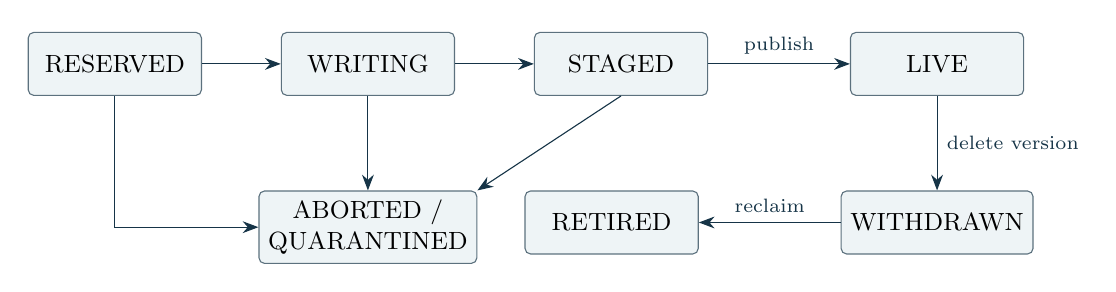
\begin{tikzpicture}[st/.style={draw=ink!70,rounded corners=2pt,fill=pale,align=center,minimum height=8mm,minimum width=22mm,font=\small},arr/.style={-{Stealth[length=2mm]},ink}]
\node[st] (res) {RESERVED};
\node[st,right=10mm of res] (wr) {WRITING};
\node[st,right=10mm of wr] (stg) {STAGED};
\node[st,right=18mm of stg] (live) {LIVE};
\node[st,below=12mm of live] (withdrawn) {WITHDRAWN};
\node[st,left=18mm of withdrawn] (retired) {RETIRED};
\node[st,below=12mm of wr] (ab) {ABORTED /\\QUARANTINED};
\draw[arr] (res) -- (wr);
\draw[arr] (wr) -- (stg);
\draw[arr] (stg) -- node[above,font=\scriptsize]{publish} (live);
\draw[arr] (live) -- node[right,font=\scriptsize]{delete version} (withdrawn);
\draw[arr] (withdrawn) -- node[above,font=\scriptsize]{reclaim} (retired);
\draw[arr] (res.south) |- (ab.west);
\draw[arr] (wr) -- (ab);
\draw[arr] (stg.south) -- (ab.north east);
\end{tikzpicture}
\caption[Version lifecycle]{Key deletion changes the object head to a separate delete marker; it does not change an older version's state. Version withdrawal and physical retirement require \rr{PUB-005}. Staged records may be durable without being publicly readable.}\label{fig:pubstates}
\end{figure}
\req{PUB-001}{R1-B}{T-08}{PostgreSQL controls logical namespace and visibility. Public bucket names and object keys \mustnot\ be used directly as filesystem paths.}
\req{PUB-002}{R1-B}{T-08, T-11}{Staging proceeds as follows. (1) \code{BeginEncryptedUpload} creates an intent with tenant, actor, subject, delegation, assigned object, logical-version, crypto-version and blob IDs, encrypted-attempt ID, expected generation/current version, metadata revision and idempotency key. (2) Authorize create or new-version and assign protected metadata. (3) The client constructs the exact bound ciphertext, signed descriptor and one independent envelope per object or unit and recipient. (4) \code{FinalizeEncryptedUpload} validates signatures, exact identifiers, format, ciphertext digest/length and envelope references, obtains the backend durable receipt, and requires every initial envelope to satisfy the same caller-share/create and target-recipient read/receive-key checks as \code{PublishRecipientEnvelope} under \rr{KEY-012} and \rr{RES-009}. Target eligibility uses the trusted intended committed state within this upload plan, never a staged-data read grant. The version and its envelopes remain unpublished until the complete fresh commit succeeds. No upload route accepts a payload decryption key.}
\req{PUB-003}{R1-B}{T-08, T-11}{Commit obtains a fresh decision for object publication and every initial envelope. Under \rr{DAT-007}, one transaction checks expected generation/current version, metadata, caller and target-principal revisions, recipient-key state, delegation, policy epoch, recovery incarnation, decision expiry and conditional-write preconditions. A missing, stale or misbound check aborts. It atomically publishes the version and approved envelopes, updates the head, consumes the intent and appends audit/outbox records. The same boundary publishes newly staged document units under \rr{DOC-002}. Initial envelopes retain all \rr{KEY-012} checks; success requires the durability barrier.}
\req{PUB-004}{R1-B}{T-08}{Only a committed LIVE version is eligible for ordinary reads. A durable STAGED catalog record, finalized backend blob or failed commit grants no visibility; pending versions and envelopes remain inaccessible through every route.}
\req{PUB-005}{R1-B}{T-08}{Key deletion publishes a separate current-head delete marker and advances the head generation; historical LIVE versions remain readable only with historical rights. Explicit version deletion checks version-delete permission, retention and references, then durably changes that version to WITHDRAWN and schedules reclamation. Deleting the current version also leaves a head marker, never restores an older version. Physical removal follows the durable withdrawal and fresh retirement guards; only confirmed removal marks RETIRED.}
\req{PUB-006}{R1-B}{T-08}{Garbage collection uses catalog references, intents, withdrawals and a grace period; file age alone is insufficient. Reconciliation is idempotent across blob finalization and catalog commit. Expired RESERVED, WRITING or STAGED attempts can be aborted under expected-state checks. Restore reconciles catalog and blobs or quarantines mismatches, and reopens access only under \rr{AVL-008}.}
\req{PUB-007}{R1-B}{T-08}{\code{If-Match} and \code{If-None-Match} apply to the committed logical version and its documented ETag, not to a staging file. Conflicting commits serialize with row locks or compare-and-swap and a fixed lock order, and two concurrent overwrites \mustnot\ both publish against the same obsolete expected generation. An ETag is an opaque identifier and is not promised to be an MD5; the server stores ciphertext checksums only. A plaintext digest, if needed by a client, stays inside its encrypted metadata and is verified locally.}
\req{PUB-008}{R1-B}{T-08}{An upload follows RESERVED, WRITING, STAGED and LIVE; any pre-LIVE state may end in ABORTED or QUARANTINED. Explicit version deletion follows LIVE to WITHDRAWN to RETIRED. Delete markers belong to the object-head history, not this version lifecycle. Transitions use expected-state checks, and no state change retargets immutable bytes (Figure~\ref{fig:pubstates}).}
\req{PUB-009}{R1-B}{REV}{The first release does not claim regulatory WORM or Object Lock compliance.}

\subsection{Object backend contract}
\begin{lstlisting}
// Logical contract. All requests carry verified workload bindings.
type ObjectBackend interface {
    Begin(ctx context.Context, req BeginRequest) (StagedWriter, error)
    Finalize(ctx context.Context, req FinalizeRequest) (DurableReceipt, error)
    Open(ctx context.Context, req ReadRequest) (BlobReader, error)
    Remove(ctx context.Context, req RetireRequest) (RemovalReceipt, error)
}
\end{lstlisting}
\req{BKD-001}{R1-B}{T-08, T-15}{\code{Begin} binds operation, tenant, blob and placement. \code{Finalize} checks exact length and digest and returns a durable receipt only after the backend's qualified durable completion condition: for the R1 single-node store, the required file and directory flushes after an exclusively created temporary file is fully written and verified; for a later backend, its own qualified acknowledgement bound to the immutable object identity and verified content. A successful network send alone is not a durable receipt. Repeating the same identity and content is idempotent, and the same blob ID with different bytes rejects. A timeout is an unknown result reconciled by operation identity, not an assumed failed write. \code{Open} exposes exact immutable bytes, and \code{Remove} accepts only a current catalog-authorized retirement plan. The caller owns stream close, cancellation and logical publication.}
\reqn{BKD-002}{R1-B}{T-08}{R1 runs on our own single-node blob store on local disk behind this contract (decision D-02). It writes each blob to an exclusively created temporary file, checks length and digest, flushes the file and its directory, and only then returns the durable receipt; the catalog, not the file system, decides visibility. It receives only client ciphertext, and no other role has direct file access. R1 makes no zero-loss claim for blob content (N-08): losing the node loses blobs written since the last backup. A later backend (the replicated store of Part~5, or another store qualified under \rr{BKD-004}) replaces it without changing client policy semantics. Volume encryption supplements client encryption and gives no platform role a payload decryption key.}
\req{BKD-003}{R1-B}{T-08}{The local backend uses service-owned directories, restrictive permissions, descriptor-relative safe file operations and symlink and traversal protection. Finalized blobs are immutable, and file and required directory metadata are flushed before a catalog transaction publishes a LIVE reference. Storage clients have no direct filesystem or backend credentials.}
\req{BKD-004}{R1-B}{T-08}{A different backend implements the same interface and needs its own consistency and durability tests. It does not duplicate user-facing policy combination in a second storage engine.}

\reqn{BKD-005}{R1-B}{T-08, T-18}{Client payload encryption is mandatory from R1-B: every accepted upload declares the approved encrypted format, supplies its signed binding and is produced by a qualified encrypting client. Ciphertext remains ciphertext in unpublished uploads, temporary files, spill, finalized blobs, replicas and backups. No server fallback decrypts or stores payload plaintext. Backend and volume encryption also protect persistent server records, opaque envelopes and ciphertext, with an approved configuration, verification method and documented drift-detection bound. A declaration or signature proves origin and binding, not that arbitrary maliciously supplied bytes were encrypted correctly; the cryptographic guarantee assumes the qualified client follows the format. The server cannot prove payload AEAD validity without a key and does not claim to do so. Unsupported or missing profiles reject publication.}

\subsection{Documents and text units in the storage core}
Native encrypted-document and text-unit endpoints are part of R1-C. They call the same resolver and ciphertext/envelope delivery path later used by MCP; a document is a catalog projection over independently protected encrypted units, not an MCP-owned resource.
\req{DOC-001}{R1-C}{T-06, T-08}{A document version has an uploader-signed canonical manifest identifying its exact unit membership, unit/object versions, ciphertext digests and format, and declared extraction and normalization versions. Its digest is computed over the canonical core of unit entries before per-unit descriptors or signatures are added, avoiding self-reference. Each deliverable unit has an uploader-signed descriptor binding tenant, document/version, the opaque manifest digest, unit/version, ciphertext digest and crypto profile. The server verifies signatures and cross-references at publication; a subset client verifies its descriptors without receiving the hidden full manifest.}
\req{DOC-002}{R1-C}{T-08}{New document units remain STAGED, with durable receipts and nonpublic catalog records, until the document transaction atomically publishes their LIVE versions, permitted envelopes, manifest and protective references. Already-published units may be referenced after current checks, with new document-specific descriptors and recipient envelopes prepared by an authorized client holding the unit key. Reuse preserves the immutable unit ciphertext; the server cannot create missing envelopes. Every referenced unit must be LIVE at the transaction outcome, and incomplete ingestion is never exposed through raw or envelope APIs. The parent and all affected units use the same authority fence and publication preconditions; retirement honors their references.}
\req{DOC-003}{R1-C}{T-06}{The qualified client splits content at authorization boundaries into stable sections, paragraphs or independently protected entries before upload and encrypts each unit with a separate payload key. Re-splitting creates a new document version. Protected access labels and revisions remain separate mutable server records; label changes alone do not change payload bytes or confer a missing recipient envelope.}
\req{DOC-004}{R1-C}{T-09}{The initial qualified client ingestion profile accepts bounded UTF-8 text and Markdown with a recorded normalization scheme. Parsing, extraction, segmentation, classification proposals and encryption occur on the client, never in the storage or MCP server. Additional formats need a separately qualified client extractor with complexity limits and source-to-text mapping. The server checks signed declarations, sizes, references and uploader authority but cannot verify plaintext extraction quality or label correctness. There is no server converter, plaintext indexing worker or embedding-provider fallback.}
\req{DOC-005}{R1-C}{T-06}{A text collection or conversation uses the same unit model through \code{text.entry}; no separate transcript authorization store exists. Manifests, text units, source references and policy metadata are tenant-bound catalog records, and unit IDs are not bearer permissions.}
\req{DOC-006}{R1-C}{T-06}{Document permission to enumerate or read units does not grant every unit or recipient envelope. Actor, subject and delegation checks apply to the parent, selected units and envelope recipient. The encrypted original and its separate key need explicit complete-content permission under \rr{CNT-003}; this is never inferred from a unit read. Raw, preview, thumbnail, version, manifest and envelope routes preserve that boundary, and no plaintext raw-download route exists.}
\req{DOC-007}{R1-C}{T-06, T-09}{An explicit unit-ID request requires every requested ciphertext and envelope disclosure to be allowed; otherwise it returns a generic denial. An authorized-subset operation returns only permitted encrypted units, their signed descriptors and separate authorized recipient envelopes with an opaque continuation. Each envelope context names exactly one object or unit version and one recipient, and the qualified envelope plaintext contains exactly that unit's keyset; batching never creates an aggregate opaque multi-unit key bundle. The server checks the outer identity and grants; the recipient verifies the single-unit keyset format after unwrapping. The server cannot inspect HPKE plaintext or prove an authorized malicious sender has not hidden other material inside it. Responses expose no hidden IDs, positions, counts or placeholders. The full manifest is returned only when all contained metadata may be disclosed, and sensitive titles/text stay encrypted for the recipient.}
\req{DOC-008}{R1-C}{T-06}{Streaming-AEAD segments and HTTP byte ranges are not independent authorization units. If different spans need different rights they are split into separate units before publication.}

\subsection{Labels}\label{sec:labels}
Authorization needs a trusted classification for every unit. Authorized labeling and collection defaults suffice for the baseline; a classifier in an authorized client is optional. The server cannot infer classification from encrypted text. Neither an untrusted client field nor a model-generated label is authoritative.
\reqn{LAB-001}{R1-C}{T-09}{Every published unit carries a protected classification label from the tenant's label order. Publication of an unlabeled unit is rejected.}
\reqn{LAB-002}{R1-C}{T-09, T-21}{A label comes from, in order of precedence: (1) explicit labeling by an authorized principal within their delegation ceiling and at or above the collection's floor; (2) the collection or bucket default; (3) a signed proposal from a registered client-side classifier, which is advisory until accepted under (1). Client-supplied and model-generated labels are never applied directly.}
\reqn{LAB-003}{R1-C}{T-09}{A unit whose label cannot be determined takes its collection's most restrictive default, and every collection declares one.}
\reqn{LAB-004}{R1-C}{T-09}{Lowering the stored label of a unit or derived output is an explicit \code{relabel} action with its own audit record and, by default, an approval. The effective label of a derived output cannot go below its lineage maximum unless a \code{relabel} allow for that output says so (\rr{DRV-007}). Raising a label is an ordinary \code{label} action.}
\reqn{LAB-005}{R1-C}{T-09}{A label change advances the affected access revision and invalidates dependent derived-output authority under \rr{DRV-009}. Decisions, disclosure plans and stream leases bind that freshness state (\rr{DEC-006}, \rr{CNT-008}). Payload re-encryption is not required.}

\subsection{Disclosure}
\req{DSC-001}{R1-C}{T-09}{Disclosure resolves the exact document/manifest, selected units and current authority, including transitive lineage dependencies under \rr{DRV-009}; obtains the complete parent/unit and recipient-envelope checks; then admits that immutable plan under \rr{DAT-007}. Only its authorized ciphertext, descriptors and existing envelopes are returned. Verification and decryption remain client-side.}
\req{DSC-002}{R1-C}{T-09}{The server authorizes ciphertext and envelope delivery before either enters a response, shared cache or downstream route. It never returns payload plaintext to a client, MCP tool, model, reranker or embedding API. A client that decrypts an authorized package owns subsequent plaintext handling. Post-generation redaction and model instructions cannot substitute for the server's delivery checks or make client plaintext recallable.}
\req{DSC-003}{R1-C}{T-09}{The platform records ciphertext and envelope delivery with exact unit/version/recipient identities and hashes, not plaintext prompts, raw keys or documents. A managed client may submit signed outcome evidence for its own optional model calls, but the server distinguishes that report from a platform-observed event and does not claim to have observed the client's plaintext use.}
\req{DSC-004}{R1-C}{T-09}{The same final unit and recipient checks apply to every encrypted disclosure surface, including preview objects, citations, notifications and subscriptions. The server emits only authorized metadata or encrypted payloads. Client-generated previews and snippets are separate encrypted resources or local views; an unsupported surface is disabled.}
\req{DSC-005}{R1-C}{T-09}{Query caches are bound to tenant, authority, version and epoch and \mustnot\ reuse a result computed for a broader user for a narrower one. No raw totals or structural positions reveal denied units.}
\req{DSC-006}{R2}{T-09}{Once an authorized client receives a usable envelope and holds its private key, the server cannot constrain where that client sends plaintext. A destination restriction may limit which registered recipient receives an envelope; it does not enforce subsequent use by an arbitrary client. Any stronger managed-client promise requires a separately qualified runtime boundary and excludes that runtime's compromise. The baseline has no server-side plaintext model-proxy route.}

\subsection{Search}
\req{SRH-001}{R1-C}{T-09}{Server search is restricted to authorized catalog metadata whose visibility is explicit: tenant, permitted aliases, approved policy attributes and opaque object/version references. It performs no plaintext full-text, semantic or embedding search. After obtaining authorized encrypted units and envelopes, the recipient client may decrypt and search locally; its text query need not leave the client.}
\req{SRH-002}{R1-C}{T-09}{Plaintext and embedding indexes are client-side state and remain outside the server storage boundary. A qualified client protects any persistent local index with its local key custody and excludes unauthorized or undecryptable units. The server stores no plaintext snippets, embeddings or extraction cache; encrypted client indexes, if uploaded, are ordinary encrypted objects and are not server-searchable plaintext.}
\req{SRH-003}{R1-C}{T-09}{The baseline server has no remote text-search, reranking or embedding integration. A client that sends decrypted content to such a service makes an additional plaintext disclosure outside baseline storage enforcement; a managed-client extension must declare and qualify that boundary. Searchable encryption, private search and server decryption are not implied by metadata discovery.}
\reqn{SRH-004}{R1-C}{T-09}{Result values, ordering, scores and totals returned to a caller depend only on candidates that caller is authorized to see. Page shape (short or empty pages) and latency can reflect scan work over hidden candidates; they are bounded by the scan budget and tenant limits, but the platform does not claim that pagination is noninterfering with respect to hidden candidates.}

\subsection{Derived outputs and declassification}\label{sec:derived}
A client-created projection, extraction or model answer is uploaded as a new encrypted resource. R1-C enforces labels and declared lineage for registered derived resources. These controls rely on qualified cooperating clients accurately describing their computation; the server cannot recover or prove provenance from ciphertext. Possession of plaintext by an authorized client remains a trust boundary.
\reqn{DRV-001}{R1-C}{T-09, T-21}{A managed or cooperating client that creates a derived object supplies signed lineage naming all input units the operation received, and encrypts the result before upload. The server validates signer authority, references, bounds and cycles. Citations do not narrow declared lineage. Because the server never sees the plaintext computation, it cannot prove that a malicious client declared every source or that an uploaded object was independently created.}
\reqn{DRV-002}{R1-C}{T-09}{For a registered derived object, delivery of its ciphertext and recipient envelope requires the normal object/envelope checks and either (a) recipient read permission on every declared lineage unit or (b) an explicit \code{declassify} decision for that exact output, version and recipient. The owner or authorized custodian client must have created the recipient envelope; a policy allow cannot synthesize one. Declassification authorizes that delivery only and does not lower the stored label.}
\reqn{DRV-003}{R1-C}{T-09}{The managed client binds the intended recipient and conservative lineage before publishing the encrypted output. The server enforces the registered bindings without inspecting wording or inferring whether plaintext leaked. This is a provenance-based delivery rule for cooperating clients, not information-flow proof against an authorized malicious client.}
\req{DRV-004}{R2}{T-09}{Optional AI submission runs in a client or explicitly trusted managed client runtime. That client obtains permitted encrypted units and envelopes, verifies and decrypts locally, and constructs its own model request. A server may authorize the proposed recipient/model metadata, but never builds a plaintext prompt or forwards decrypted content. A managed profile binds destination and parameters; baseline storage makes no claim to police arbitrary client networking.}
\reqn{DRV-005}{R2}{T-09}{The baseline rejects a request to perform server-side \code{use-in-model} without client read capability; it has no plaintext execution path for it. A future managed-client profile may distinguish an end user from a separate authorized execution recipient, but must qualify that client's custody, output encryption and recipient-specific declassification before being enabled. It cannot be implemented by giving the storage or MCP server a decryption key.}
\reqn{DRV-007}{R1-C}{T-09, T-21}{The effective server label of a registered derived output is at least the highest effective label in its declared lineage. A collection default acts as a floor, so the effective label is the maximum of the collection default and the lineage maximum. Only an explicit \code{relabel} allow for that output can lower it, and the effective label is the one used when the output is reopened and when a context mark is updated.}
\reqn{DRV-008}{R1-C}{T-09, T-21}{Disclosure to one recipient and relabeling are separate authorizations. A \code{declassify} allow is bound to output, version and recipient and records the label reported to a qualified managed client for flow control; absent an explicit lower label, that is the lineage maximum. Lowering the stored label for everyone is a \code{relabel} action (\rr{LAB-004}).}
\reqn{DRV-009}{R1-C}{T-09, T-13, T-21}{Derived-output authority includes its complete transitive lineage. A source access, label, lifecycle or relevant declassification change invalidates dependent decisions and leases even when output bytes and revisions are unchanged. The implementation may use dependency revisions, a conservative epoch or transactional propagation, but must qualify equivalent freshness under \rr{DAT-007}, bounded traversal and cycle rejection. New delivery recomputes effective authority; ongoing delivery follows \rr{CNT-008}. Test chained derivation and a source change during an output stream.}
\req{DRV-006}{R2}{REV}{An AI provider receiving plaintext from a client is outside the ciphertext-only storage boundary. Client/provider retention, training and onward disclosure are not controlled by the storage cryptography. Managed-client lineage records describe declared provenance, not proof against hidden inputs, malicious client behavior or sensitive inference.}

\subsection{MCP as a later encrypted-content client}
The R2 MCP service is an authenticated facade over the same ciphertext and recipient-envelope API. It preserves user and delegation authority and returns the exact versions and projections a native client can obtain. A qualified client SDK or local bridge verifies the descriptors and decrypts with keys held on the client side of that boundary. A generic MCP client does not automatically understand this encrypted representation; capability negotiation either selects the qualified format or reports it unsupported. No compatibility mode returns plaintext from the server.
\begin{longtable}{@{}P{0.22\textwidth}P{0.27\textwidth}P{0.32\textwidth}P{0.08\textwidth}@{}}
\caption{Later MCP service mappings to encrypted content operations}\label{tab:mcpops}\\
\toprule MCP operation & Required action model & Returned representation & Phase\\\midrule\endfirsthead
\toprule MCP operation & Required action model & Returned representation & Phase\\\midrule\endhead
\code{documents.search} & Authorized metadata discovery only & Permitted references and metadata; no server text snippets, embeddings or plaintext query processing & R2\\
\code{documents.read} & Parent and unit read plus all recipient-envelope checks & Selected ciphertext, signed unit descriptors and existing recipient envelopes; local decryption & R2\\
\code{text.read} & Collection/entry and exact-version read plus recipient checks & Same encrypted unit package; no unguarded text endpoint & R2\\
\code{resources/list}, \code{resources/read} & Same discovery and read checks as tools & Registry-bound references and encrypted packages; no direct backend or file access & R2\\
\code{documents.export} & Complete mapping of Table~\ref{tab:keyops} & Ciphertext and envelopes for an approved compatible recipient; no server rewrapping or decryption & R2\\
\bottomrule
\end{longtable}
Optional AI assistance is a client workflow after authorized local decryption. The baseline MCP service exposes no \code{ai.ask} operation that receives or constructs plaintext context; any managed-client model integration needs its separately qualified authority and disclosure boundary.

\subsection{Sizing and scaling}
\reqn{SIZ-001}{R1-B}{T-22}{Qualification reports measured ciphertext object-service capacity and client encrypt/decrypt costs in R1-B, then unit and recipient-envelope fan-out for the reference documents in R1-C. R2 adds the independently deployed MCP service. Measurements separate server ciphertext throughput and signature checks from client HPKE wrapping/unwrapping and payload AEAD work.}
\req{SIZ-002}{R1-B}{T-22}{The \code{storage} role scales independently with bounded requests, ciphertext streams, upload/read concurrency, buffer memory, signature-verification work and tenant byte budgets. Decision replicas and backend capacity are qualified with \rr{AVL-007}; adding frontends does not imply unlimited catalog throughput. R1-C adds bounded unit and envelope fan-out and metadata discovery. The R2 \code{mcp} role has its own replica set and identity and calls the same encrypted-content API. Client compute and local indexes scale at the client; no server permission database, evaluator or plaintext cache is added for MCP.}
\begin{longtable}{@{}P{0.28\textwidth}P{0.44\textwidth}P{0.18\textwidth}@{}}
\caption{Sizing quantities (formulas; values are measured, not assumed)}\label{tab:sizing}\\
\toprule Quantity & Measurement or formula, with $u$ units per document and $c$ search candidates & Release\\\midrule\endfirsthead
\toprule Quantity & Measurement or formula, with $u$ units per document and $c$ search candidates & Release\\\midrule\endhead
Object-service capacity & Object-size distribution, concurrent streams, read/write throughput, catalog commit rate, backend latency and bounded memory per request & R1-B\\
Decision batches to read a whole document & $\lceil k/50 \rceil$, where $k$ includes the parent, $u$ unit checks and every required recipient-envelope check & R1-C\\
Decision batches per metadata page & $\lceil c/50 \rceil$ before any prefilter (\rr{CNT-007}) & R1-C\\
Blobs, catalog rows per ingest & $u$ blobs, $u$ unit rows, 1 manifest & R1-C\\
Recipient envelopes & Up to $u \times r$ client-created HPKE envelopes for $r$ authorized recipients; server stores and authorizes delivery only & R1-C\\
Client cryptographic work & $u$ independent payload encryptions at ingest; selected-unit envelope unwraps and payload decryptions at recipients & R1-C\\
Durable receipts per publication & Backend-defined; 2 per immutable blob with the custom store & R1-B, R3\\
Reference documents & $u = 10$, $u = 1{,}000$ and $u = 10{,}000$ & R1-C\\
\bottomrule
\end{longtable}

% Expanded source: p04-custody

\section{Client encryption and authorized envelope delivery}\label{sec:custody}
Clients encrypt content before upload and decrypt it after download. This is mandatory for the native object API in R1-B and for independently protected document and text units in R1-C. R2 MCP transports the same encrypted objects; it does not introduce encryption or move decryption to the server. TLS additionally protects authenticated connections, but payloads remain ciphertext inside the platform, its internal network, backing stores and backups.

In the supported data path, no platform role receives plaintext payloads, raw data keys or recipient private keys. The \code{keys} role is an authorization and envelope-delivery service: it stores and returns opaque, client-created recipient envelopes. It cannot unwrap a data key, rewrap one for another user, or recover plaintext. Independently authored Go code integrates qualified streaming AEAD, HPKE and signature libraries in the client SDK; it does not invent cryptographic primitives.

\subsection{Mandatory client custody}
Each immutable object version has a fresh data key (keyset). In R1-C each separately protected text-unit version is an ordinary immutable object with its own fresh keyset. A client encrypts the payload under that keyset and wraps the keyset to each explicitly approved recipient public key using HPKE. The server stores ciphertext and opaque recipient envelopes with authenticated bindings. There is no shared bucket data key, server master decryption key or whole-document data key that unlocks independently protected units.

\begin{longtable}{@{}P{0.27\textwidth}P{0.63\textwidth}@{}}
\toprule Boundary & Material and responsibility\\\midrule\endhead
Owner or authorized recipient client & Plaintext, its private keys and the data keys it can unwrap; encrypts, verifies and decrypts locally\\
Optional organization custodian client & An independently controlled client with an explicit recipient envelope; can recover or authorize new recipient envelopes only for versions it can already decrypt\\
Platform storage role & Ciphertext, signed descriptors and catalog bindings; verifies publication, access and durability without decrypting\\
Platform \code{keys} role & Opaque recipient envelopes and public-key records; authorizes publication and delivery without unwrap capability\\
MCP and tool services & Authorized encrypted packages and permitted routing metadata; no plaintext conversion or private-key custody\\
Backing storage and backups & Ciphertext and protected metadata; provider encryption is additional protection, not a substitute for client encryption\\
\bottomrule
\end{longtable}
\req{CRY-001}{R1-B}{T-10}{Client encryption is the only payload custody profile. Missing, unknown, server-decryptable or unencrypted profiles reject publication. Neither an API flag nor a privileged server role can request plaintext storage or server-side decryption. Profile, suite and format are recorded for each immutable version and checked on every encrypted-package operation.}

\subsection{Payload cipher suite and immutable binding}
\req{CRY-002}{R1-B}{T-10}{The client SDK uses a qualified streaming AEAD (initial candidate: Tink AES-256-GCM-HKDF with 1 MiB segments). The library handles nonce generation, key derivation, segment authentication and final-segment marking; project code \mustnot\ reproduce its chunked encryption. The module checksum and format tests are pinned.}
\req{CRY-003}{R1-B}{T-10}{Payload additional authenticated data (AAD) binds the tenant, object, crypto version, cipher suite and format under a versioned domain identifier. The same binding appears inside each recipient key package, preventing substitution across those identities. Mutable display names, classifications and envelope generation are excluded so that authorized metadata and recipient changes do not rewrite payloads. AAD is authenticated, not confidential; secrets and personal data do not belong in it. The exact field encoding is retained in the companion \code{crypto-format-profile.tex} and is qualified with the client wire contract under \rr{RCP-007}.}

\req{CRY-004}{R1-B}{T-10}{A published encrypted version binds tenant, object, logical version and crypto-version IDs; suite and format; ciphertext digest and length; uploader signing identity; and signed ciphertext descriptor. Its envelope records additionally bind recipient fingerprint and key version, envelope generation, opaque HPKE ciphertext and the origin signature. Logical versions, crypto versions, recipient-key versions and envelope generations remain distinct.}
\req{CRY-005}{R1-B}{T-11}{Raw keysets and recipient private keys never enter platform APIs, logs, persisted records or process memory. Only authorized clients handle them. A public key or client-supplied opaque envelope is not authority to read, create or share a resource; the server checks the exact operation independently of possession of those bytes.}

\subsection{Client-generated keys and server envelope service}
\reqn{KEY-001}{R1-B}{T-10, T-12}{The baseline uses flat recipient wrapping: the client generates a fresh data keyset for every immutable object version and, in R1-C, every protected unit version, then creates a separate HPKE envelope for each explicitly approved recipient. Every envelope contains exactly one keyset for one immutable object or unit version and one recipient; a batch is a container of independently authorized envelopes, never a multi-unit encrypted key bundle. Data keys are not shared across tenants, objects or versions. A document-level KEK hierarchy is deferred under D-09; any later proposal keeps KEKs solely in authorized clients, preserves independent unit release, and cannot give platform roles an unwrap capability.}
\req{KEY-002}{R1-B}{T-11}{The envelope service authenticates the calling client or service and requires a signed decision for the exact delivery or publication operation. It resolves recipient fingerprints and envelope identities from the canonical registry and catalog, verifies current revisions, and returns only the exact stored envelope for that recipient. It never accepts a caller-provided key-server URL, unwraps an envelope, or substitutes a broader recipient.}
\req{KEY-003}{R1-B}{T-11}{Before encryption, an upload intent binds the stable object ID and allocates fresh logical-version, crypto-version and blob IDs for that encrypted attempt. Exact retries reuse those IDs and the identical ciphertext; a restarted encryption attempt requires a new intent with fresh version, crypto-version and blob IDs. The server validates ciphertext length and digest, signed descriptor, uploader authority, recipient bindings, durable receipts and publication preconditions; it cannot verify the inner AEAD tag, plaintext format, plaintext classification or whether an opaque envelope decrypts. Those properties depend on the authorized publishing client and are checked by receiving clients where possible. Outer format validation cannot prove that a malicious uploader encrypted arbitrary submitted bytes; the confidentiality guarantee assumes a trusted compatible publishing client, not truthful labels on hostile uploads. Pending ciphertext and envelopes are not eligible for general reads.}
\req{KEY-011}{R1-B}{T-10, T-11}{The client and server operations behave as in Table~\ref{tab:broker}. Server operation names and API types \mustnot\ imply plaintext key generation, unwrap or rewrap.}
\reqn{KEY-012}{R1-B}{T-11}{Ciphertext access, recipient-envelope delivery and sharing are separate compound operations with the check sets of Table~\ref{tab:keyops}. The storage and envelope services verify the complete applicable signed result, exact operation and recipient bindings; absence of a required check denies. Initial envelopes supplied with an upload pass the same publication checks as later envelopes, including recipient-revision checks at commit. Publisher share/create checks use the authenticated publisher actor and subject; target read/read-units and receive-key eligibility use the server-resolved recipient principal through \rr{RES-009}. Each signed check names its evaluated principal and current identity revision. Initial-upload eligibility is evaluated for the exact planned published state bound to the intent, not as permission to read STAGED content. An eligibility result grants no delegation or present read authority; caller-supplied recipient attributes cannot replace authoritative resolution. R1-C applies the same checks to both the document boundary and every selected unit.}
\begin{longtable}{@{}P{0.30\textwidth}P{0.47\textwidth}P{0.13\textwidth}@{}}
\caption{Compound operations for encrypted content}\label{tab:keyops}\\
\toprule Operation & Required checks and bindings & Enforcer\\\midrule\endfirsthead
\toprule Operation & Required checks and bindings & Enforcer\\\midrule\endhead
Ciphertext read & \code{read} on the exact object version; for documents, parent \code{read-units} and \code{read} on every selected unit; permitted metadata projection & Storage\\
\code{GetRecipientEnvelope} & Caller read and envelope-release checks; separate target-recipient read/read-units and \code{receive-key} eligibility under \rr{RES-009}; exact recipient fingerprint and current revisions & Envelope service\\
\code{PublishRecipientEnvelope} & Publisher \code{share} on the exact object or document and selected units, plus envelope \code{create}; separate target-recipient read/read-units and \code{receive-key} eligibility; client-origin signature and exact ciphertext binding & Envelope service\\
Remote package export & \code{export} on the object or document version and \code{export-key} on each selected unit where applicable, in addition to the applicable read and envelope-delivery checks; only an already-created envelope for that recipient & Storage and envelope service\\
\bottomrule
\end{longtable}
\begin{longtable}{@{}P{0.29\textwidth}P{0.61\textwidth}@{}}
\caption{Client and envelope-service operations}\label{tab:broker}\\
\toprule Operation & Required behavior\\\midrule\endfirsthead
\toprule Operation & Required behavior\\\midrule\endhead
\code{BeginEncryptedUpload} (server) & Authorize create or new-version; bind stable object ID and allocate intent, logical-version, crypto-version and blob IDs; return parameters without generating or receiving a data key\\
\code{EncryptObjectVersion} (client) & Generate keyset; stream-encrypt with exact AAD; create recipient envelopes for independently verified approved public keys; sign ciphertext descriptor and envelope contexts\\
\code{FinalizeEncryptedUpload} (server) & Verify signature, intent, profile, ciphertext digest/length and durable receipt; apply the full initial-envelope checks. Publish at the authorized object commit, or retain document units STAGED until the atomic document commit\\
\code{GetRecipientEnvelope} (server) & Verify the full signed delivery decision and freshness; return the existing opaque client-created envelope with its origin evidence; record delivery audit\\
\code{CreateRecipientEnvelope} (client) & Obtain a usable existing envelope and verify source; authorize sharing; verify target fingerprint independently; unwrap locally and create a new HPKE envelope for the same data key and exact version; sign its context\\
\code{PublishRecipientEnvelope} (server) & Recheck publisher authority, target-recipient eligibility and both identity and recipient revisions at commit; verify client origin and bindings; atomically publish opaque envelope, generation and audit record\\
\code{RetireEnvelope} (server) & Authorize retirement; withdraw future delivery, advance revisions and record audit; preserve required recovery references without claiming to erase client copies\\
\bottomrule
\end{longtable}

An owner or organization custodian is a client connected to the same system, not a privileged server decryption role. It can create a new recipient envelope only if it already holds the corresponding private key or a usable data key. Approval alone cannot manufacture access to an existing encrypted version. If no such client is available, the share operation remains unavailable; there is no emergency server unwrap.

\subsection{Client key custody and failure handling}
\req{KEY-004}{R1-B}{T-10, T-12}{Recipient-key rotation is performed by an authorized client: decrypt an existing envelope locally, verify the newly approved recipient key, create and sign a replacement envelope, and publish it under the expected envelope and recipient revisions. The data key and ciphertext identity remain unchanged. The platform cannot rewrap it itself, and rewrapping the same disclosed data key does not revoke old access.}
\req{KEY-005}{R1-B}{T-10, T-12}{The client uses its approved private-key store and a qualified cryptographic library. Optional hardware or an organization-operated key service belongs to the explicitly trusted client custody boundary and is selected under D-08; it is not a platform KMS unwrap dependency. No platform identity has permission to use recipient private keys. Envelope encryption is randomized; retries reuse the persisted encrypted attempt and operation identity, not convergent encryption or caller-chosen nonces.}
\req{KEY-006}{R1-B}{T-10}{Inside HPKE, a versioned key package carries the exact payload binding and one library-serialized binary keyset, with explicit bounded lengths. The receiving client rejects inconsistent lengths, trailing bytes, unknown versions, keysets above 64 KiB, extra keys or keysets, and any suite, binding or streaming-AEAD-template mismatch before use. The exact field ordering and integer encodings are retained in \code{crypto-format-profile.tex}. Servers treat the package as opaque and enforce only outer encoding and size bounds; they cannot prove that a hostile publisher put only the declared key inside HPKE.}
\req{KEY-007}{R1-B}{T-19}{Clients protect keys and plaintext against logs, traces, dumps and support exports and restrict debugging of decryption processes. Raw key buffers have an explicit owner and lifetime, avoid strings and unnecessary copies, and are cleared when the API permits. Perfect zeroization of Go or library-managed copies is not promised. Server diagnostics contain only permitted metadata and opaque-envelope identifiers; TLS protects all client and service connections in addition to payload encryption.}
\reqn{KEY-013}{R1-B}{T-11}{Process and credential boundaries prohibit all platform roles, including storage, decision, MCP, tools, maintenance and envelope delivery, from receiving payload plaintext or unwrapped data keys. The client verifies both the encrypted package's origin and its own recipient binding before decryption. Deployments \mustnot\ silently host a plaintext-processing custodian or model inside the platform and describe it as client-only encryption.}
\reqn{KEY-014}{R1-B}{T-11, T-13}{Server caches contain only ciphertext, opaque envelopes or permitted metadata, never plaintext keysets. Every new delivery still checks current identity, recipient status, resource and envelope revisions, policy epoch and expiry. Client key retention follows the client's explicit custody policy; the platform does not claim that a client-side cache expires cryptographically when a grant or server lease expires.}
\reqn{KEY-015}{R1-B}{T-11, T-13}{A missing recipient envelope, unavailable client private key, failed signature or AEAD validation, stale authority, or unavailable authorization dependency prevents the corresponding delivery or decryption. No path falls back to a server-held key, another recipient, an older weaker profile or plaintext transfer. Client-side key-store failure does not cause private keys to be uploaded to the platform.}

\subsection{Client decryption, streaming and copy}
\req{CRY-006}{R1-B}{T-10}{The client releases plaintext only after verifying its signed origin and exact ciphertext digest and length. The baseline therefore receives the complete ciphertext into bounded, access-restricted encrypted-content storage before decrypting it as authenticated segments; it rejects oversized objects, insufficient temporary capacity, incomplete transfers and digest failures without releasing plaintext. Temporary ciphertext is cleaned up under the client custody policy. An alternative streaming profile needs equivalent authenticated origin binding and separate qualification. Overall success additionally requires valid AEAD stream termination. Wrong AAD or key, corruption, segment reordering, duplication, truncation and forged final segments fail. Memory and concurrent work remain bounded. Qualification includes temporary-storage demand and time to first plaintext; server leases govern delivery, not subsequent use of retained bytes or keys.}
\req{CRY-007}{R1-B}{T-10}{Retrying an upload resends identical ciphertext and envelopes for the same encrypted attempt. Restarting encryption requires a new intent and fresh logical-version, crypto-version and blob identities, together with a fresh keyset; it cannot overwrite an earlier attempt or change the bytes associated with an existing idempotency identity. The baseline reads complete encrypted streams. Ciphertext range transfer and client-side authenticated range assembly require a separately qualified profile; the server never implements plaintext ranges by decrypting.}
\req{CRY-008}{R1-B}{T-10}{AAD binds the logical object and crypto version, so ordinary byte copy to a new object is not a valid encrypted object. An authorized client decrypts locally and re-encrypts under a fresh destination key and binding, then publishes a new version; otherwise copy rejects. Storage repair may copy identical ciphertext for the same immutable identity. A future alias feature needs explicit same-ciphertext semantics and cannot weaken identity binding.}

\subsection{Rotation, compromise and revocation}
\req{KEY-008}{R1-B}{T-12}{The platform and authorized clients respond to each event as in Table~\ref{tab:rotation}.}
\begin{longtable}{@{}P{0.24\textwidth}P{0.66\textwidth}@{}}
\caption{Key events and required responses}\label{tab:rotation}\\
\toprule Event & Required response\\\midrule\endfirsthead
\toprule Event & Required response\\\midrule\endhead
Recipient-key rotation & Owner or custodian client creates envelopes for independently verified replacement keys; publish with revision checks; retain recovery access according to explicit custody policy\\
Content-signing-key rotation & Retire signing authority while preserving trusted historical verification bindings; current access remains separately authorized (\rr{RCP-011})\\
Content-signing-key compromise & Stop new publications; quarantine affected origin evidence until reviewed under \rr{RCP-011}; never trust a claimed signing time alone\\
Data-key compromise & Authorized client generates a fresh data key and ciphertext version; new envelopes over the old key do not repair disclosure; retained old ciphertext remains exposed\\
Recipient private-key compromise & Revoke future deliveries and new sharing to that key; assess every historical envelope recoverable with it; use fresh data and recipient keys for replacement versions where needed\\
Grant or user revocation & Block new ciphertext fetches and envelope deliveries at the effective revision; plaintext, keys and ciphertext already obtained cannot be recalled\\
Deletion or crypto-erasure & Track ciphertext, envelopes, replicas, backups and retention; server deletion cannot prove destruction of keys or copies held by clients\\
Lost client keys & Use only an explicitly provisioned recovery or custodian recipient; if every usable private key and recovery path is lost, the content is unrecoverable\\
\bottomrule
\end{longtable}
\req{KEY-009}{R1-B}{T-11}{Envelope publication, delivery, rotation and retirement record resource and version, actor and subject, decision and operation IDs, policy epoch, recipient fingerprint, envelope generation, origin signer and outcome, without plaintext or keys. Delivery audit proves release of encrypted material, not that a recipient decrypted or read it.}
\req{KEY-010}{R1-B}{T-13}{Revocation blocks new server-mediated fetches and envelope deliveries, including retries and cached responses after authority expires. It does not erase client private keys, exported data keys, retained ciphertext, plaintext or derived answers. Expiry in a signed delivery receipt is not a self-destructing key. Static-recipient HPKE does not promise forward secrecy after compromise of the recipient private key. Re-encrypting future versions limits future exposure but does not repair already-copied material.}

\subsection{Atomic lifecycle, format migration and recovery}
\reqn{KEY-016}{R1-B}{T-10, T-12}{The catalog binds one exact client-encryption profile, payload crypto version, suite and format per immutable version. Publishing a replacement recipient envelope verifies the authorized client signature and expected recipient and envelope revisions, then atomically updates the envelope generation and audit record. Replacement or retirement in one document context does not replace or retire envelopes required by another retained document version. Re-encryption creates fresh keys and an immutable ciphertext version in the client, followed by the ordinary publication checks. A partial rotation cannot publish an envelope bound to another ciphertext or recipient.}
\reqn{CRY-009}{R1-B}{T-10, T-12}{Migration between qualified client-encryption formats is an authorized client read-and-new-version operation. The client verifies the source, decrypts locally, encrypts with fresh state and publishes signed descriptors and new recipient envelopes. The original remains current until the new version commits. R1-C document migration publishes a new manifest only when every referenced unit version is ready. There is no R1 server-plaintext profile to migrate and no server-side conversion path.}
\reqn{CRY-010}{R1-B}{T-11, T-13}{Migration preserves tenant and logical resource identity, labels, current access controls and historical restrictions. The migrating client receives only explicit source-read, destination-publication and share authority. The catalog records the profile of every retained version and migration coverage; tightening the minimum accepted profile rejects new delivery of nonconforming versions. Clients cannot request a weaker format as a fallback, and a retained older representation is not declared erased or migrated.}
\reqn{KEY-017}{R1-B}{T-12, T-18}{Recovery restores a mutually consistent catalog, signed descriptors, ciphertext, opaque recipient envelopes and historical content-signing trust records. It verifies identities, digests, signatures and references and quarantines missing or mismatched records. Admission reopens only under the recovered-authority rules of \rr{AVL-008}; restoring old records cannot silently reactivate revoked authority. A separately controlled authorized client demonstrates decryption using its own private key or an explicitly provisioned organization-custodian envelope; the restore service never receives that key or plaintext. Restore qualification covers retained versions across recipient and content-signing-key rotation, compromised-signer handling, and continued denial of unauthorized server deliveries. Client recovery custody and private-key backups remain separate; platform backups alone cannot recover lost client private keys.}

\subsection{Recipient enrollment, HPKE and authenticated origin}
Online policy checks govern ciphertext and envelope delivery; recipient-bound HPKE ensures that those server-held envelopes are usable only by holders of the corresponding private keys. Neither mechanism controls an authorized recipient's later copying or independent sharing of plaintext. The owner must explicitly choose any organization recovery recipient; there is no implicit platform escrow.

\req{RCP-001}{R1-B}{T-03, T-11}{Recipient public-key encryption, client content signing, request authentication and server decision signing are separate key purposes. Signing or OAuth proof keys are not interchangeable with X25519 HPKE encryption keys. Each registry record binds tenant, principal or workload, fingerprint, purpose, suite, validity, status and revocation revision. A public key identifies an encryption recipient but does not itself grant access.}
\req{RCP-002}{R1-B}{T-03, T-11}{Enrollment and rotation use an authenticated authorized operation and validate public-key format and suite. Activation requires trusted provisioning or proof of the private key through a server-generated, short-lived, one-use challenge bound to identity and fingerprint, completed over the authenticated session. Before encrypting or sharing, the publishing client additionally verifies the recipient fingerprint through owner-approved provisioning or an independently trusted organization-signed directory and pins that binding. Possession proof and a platform-served directory alone do not establish the intended recipient: a compromised server could substitute a key it owns. Recipient rotation therefore requires explicit verification and cannot silently replace a pinned key.}
\req{RCP-003}{R1-B}{T-03}{Issuer verification keys come only from configured trusted discovery or JWKS endpoints with bounded refresh, redirects and egress and with issuer, audience, purpose and algorithm checks. Caller-supplied \code{jku}, \code{x5u} and arbitrary key-server URLs are never dereferenced. Issuer-key discovery is not a recipient directory or authority to replace a client's pinned recipient or content-signing key.}
\req{RCP-004}{R1-B}{T-10, T-11}{The client creates recipient envelopes using a qualified Tink hybrid-encryption implementation with HPKE suite \code{DHKEM_X25519_HKDF_SHA256_}\allowbreak\code{HKDF_SHA256_AES_256_GCM}. HPKE encrypts the small data-key package, not the bulk object. It does not by itself authenticate the author, so client-origin signatures and trusted signer bindings are required as in \rr{RCP-008}.}
\req{RCP-005}{R1-B}{T-11}{The published recipient envelope binds exact tenant, object and logical and crypto versions, ciphertext digest and length, profile, recipient fingerprint and key version, envelope generation and authorized sharing client. For a document unit, its identity additionally includes the document, document version and opaque manifest digest; distinct contexts coexist even when they reference the same immutable unit and recipient. It contains exactly that one unit's keyset; independently authorized envelopes for multiple units may be returned together but are never combined inside one HPKE ciphertext. The envelope service returns stored envelopes only after all applicable checks of Table~\ref{tab:keyops}; it cannot manufacture a missing recipient envelope or expand section-only rights to other units.}
\req{RCP-006}{R1-B}{T-10}{The client serializes a versioned Protobuf \code{RecipientEnvelopeContextV1} once under the explicit application wire profile of \rr{RCP-007}, with fixed UUID and byte representations, timestamp units and exactly one object-or-unit version and recipient binding. It signs those exact context bytes with the HPKE ciphertext; receivers verify received bytes rather than reserializing them. Protobuf serialization is not assumed canonical~\cite{protobufCanonical}. Strict wire validation rejects unknown or duplicate fields, aggregate bindings, unsupported values and oversized fields before a permissive decoder can discard ambiguity. HPKE context information is a domain-separated SHA-256 of the context bytes. A batch is a bounded, uniquely ordered list of separate envelopes, each independently validated and authorized. Stable encrypted context contains no expiring decision: delivery carries a separate signed receipt bound to envelope digest, operation, decision, audience, current authority and recovery revisions, and expiry.}
\req{RCP-007}{R1-B}{T-10}{Before the encrypted-package profile is enabled, its versioned interoperability contract freezes the message schemas, parsing rules and limits, signature and digest algorithms, domain separation, fingerprint encoding, Tink framing and key encoding, and exact positive and negative wire examples. Actual client/server interoperability tests qualify that contract and the pinned library versions; naming Protobuf, Tink or HPKE alone is not qualification. Algorithm or framing changes require a new reviewed profile rather than an implicit fallback. The native encrypted-package client is required in R1-B. An R2 MCP client needs a compatible local bridge or SDK to decrypt; links point only to authenticated delivery endpoints.}
\req{RCP-008}{R1-B}{T-10, T-11}{The publishing client signs the ciphertext descriptor and each recipient-envelope context and ciphertext with a separately registered content-signing key. Receivers verify origin against independently trusted signer bindings, applying \rr{RCP-011}, and verify the ciphertext digest, exact AAD and recipient binding before releasing plaintext under \rr{CRY-006}. A document unit may use a signed descriptor bound to the opaque full-manifest digest without exposing denied entries. The manifest digest covers its explicitly encoded core before descriptors or signatures are added, avoiding self-reference. A server decision signature attests authorization and delivery metadata, not client content origin. Client software distribution and updates preserve this boundary; compromised client software can expose plaintext.}
\req{RCP-009}{R2}{T-03}{Sender-constrained OAuth such as DPoP is an optional negotiated transport profile using a maintained implementation and enforcing signature, method, URI, token-key binding, time, nonce and replay rules. It neither grants resource permission nor automatically binds the request body or separate HPKE recipient key. It is not required for baseline client encryption, and base MCP support is not assumed.}
\req{RCP-010}{R1-B}{REV}{ABE, proxy re-encryption and client KEK hierarchies are deferred. A later proposal needs its own threat model, maintained-library qualification and measured need. It cannot introduce platform plaintext or private-key custody, and it is not a parallel default implementation.}
\reqn{RCP-011}{R1-B}{T-10, T-12, T-18}{Content-signing keys have immutable identity and purpose bindings and distinct active, retired and compromised states. Routine rotation or principal removal prevents new signing authority but preserves independently trusted historical verification records for retained content; it grants no current read access. Compromise blocks new publications signed by that key and causes affected historical signatures to fail closed unless a reviewed, object-specific disposition establishes trustworthy prior publication or fresh endorsement by an authorized client. An uploader-supplied timestamp is not that evidence. Clients apply authenticated trust updates with a declared freshness policy, and offline verification is not claimed to establish current revocation status. Recovery preserves these records and never converts a compromised key back to active.}
\begin{longtable}{@{}P{0.23\textwidth}P{0.43\textwidth}P{0.20\textwidth}@{}}
\caption{Cryptographic choices}\label{tab:abe}\\
\toprule Approach & Fit and limit & Decision\\\midrule\endfirsthead
\toprule Approach & Fit and limit & Decision\\\midrule\endhead
Client AEAD plus recipient HPKE & Independent version keys, opaque server storage, explicit client-managed sharing; retained keys remain usable offline & Required baseline\\
TLS on every connection & Protects authentication and transport metadata in addition to encrypted payloads; does not replace client encryption & Required\\
Client or organization custodian & Recovery and new sharing only for versions with an explicit usable custodian envelope & Optional, owner-approved\\
Ciphertext-policy ABE & Offline attribute-key infrastructure does not directly implement arbitrary dynamic policies or revoke retained keys & Deferred\\
Proxy re-encryption & Could transform recipient envelopes without server plaintext, but adds another cryptographic lifecycle and trust model & Deferred\\
Client document KEK & May reduce envelope work but broadens compromise impact; may never become a platform-held master key & Deferred under D-09\\
\bottomrule
\end{longtable}

% Expanded source: p05-storage

\section{S3 compatibility and replicated storage}\label{sec:storage}
Part~5 extends the object-storage product in R3. The native storage API, durable backend and shared fine-grained authorization already ship in R1. Client payload encryption and opaque envelope custody are part of R1; R2 adds the MCP service without replacing that foundation. S3 is an additional protocol facade over the same content service. A custom replicated blob backend is a separate, optional replacement for the R1 single-node store. Neither S3 compatibility nor owning a replication engine defines whether the product is object storage. Each extension is admitted independently through the existing backend and content contracts; adding S3 does not require changing the byte-storage engine, and changing the backend does not change client policy semantics.

\subsection{S3 compatibility profile v1}\label{sec:s3}
Implement protocols from public specifications with an explicit small surface. Version~1 supports header-signed SigV4 over TLS, bounded known-length single-chunk PUT, GET and HEAD, logical deletion, explicit historical version operations and ListObjectsV2 with filtered visibility. PUT bodies are client-produced encrypted packages; ordinary GET returns ciphertext, not transparently decrypted file bytes. A qualified client SDK additionally obtains the authorized signed descriptors and recipient envelope through the content/envelope API and decrypts locally. A stock S3 client can transfer ciphertext but does not thereby implement this encrypted-object profile. Bucket creation initially uses the control API. Multipart, server-side copy, presigned requests, browser POST, ACLs, public bucket policies, SigV2, SigV4a, streaming-signature modes and directory-bucket extensions are disabled until separately qualified.
\req{S3P-001}{R3}{T-07}{The server advertises ``S3 API subset, client-encrypted content profile v1''. Unsupported requests receive documented protocol errors, the restrictions appear in client configuration examples and tests, and the platform promises neither default S3 client compatibility nor transparent plaintext reads.}
\req{S3P-002}{R3}{T-07}{The profile requires an explicit SHA-256 payload hash (including the empty-body hash) and rejects \code{UNSIGNED-PAYLOAD}, every \code{STREAMING-*} mode and unimplemented checksum or trailer encodings. The ciphertext body digest and uploader descriptor binding are verified before publication; SigV4 authenticates the request but does not prove payload AEAD validity or plaintext correctness. The client verifies AEAD tags after download.}
\req{S3P-003}{R3}{T-07}{The SigV4 verifier is a new security-sensitive module built from the documented canonicalization and verification requirements; the AWS Go SDK signer is a client helper, not a server verifier. It validates credential scope, service and region, timestamp and skew, signed-header coverage, request canonicalization, signature (with constant-time comparison), credential state and payload integrity. S3 object paths are not normalized, because duplicated slashes and encoded bytes can distinguish keys.}
\req{S3P-004}{R3}{T-07}{S3 routing uses a dedicated raw handler that preserves exact signing and object-key semantics. Go's \code{ServeMux} cleans and redirects some paths and is not used for S3 routing, although management APIs may use it.}
\reqn{S3P-005}{R3}{T-07}{The compatibility matrix names each tested client (for example the AWS SDK for Go v2, boto3 and rclone) with the exact settings it needs, including request-checksum behavior, because recent AWS SDK releases enable default request checksums and chunked trailers that the profile rejects. Failures under default settings are documented.}
\req{S3P-006}{R3}{T-07}{Protocol tests cover duplicate headers and query parameters, percent encoding, literal plus, Unicode, host ambiguity, missing signed security headers, truncation, oversized bodies and time-bound credentials, and use independently authored cases and external client tests.}
\req{S3P-007}{R3}{T-07}{A read authenticates the request, resolves a committed logical object and version, loads trusted attributes, evaluates read or stat, and opens exactly that immutable ciphertext blob, binding resource generation, metadata revision, profile and crypto version to the decision. Recipient-envelope retrieval remains separately authorized under Table~\ref{tab:keyops}; an S3 credential is not a decryption key.}
\req{S3P-008}{R3}{T-07}{Conditional writes (\code{If-Match}, \code{If-None-Match}) map to the publication compare-and-swap of \rr{PUB-007}, and the platform documents its precise error mapping to S3 behavior.}
\req{S3P-009}{R3}{T-07}{Multipart and copy enter the compatibility matrix only after dedicated tests. Multipart needs an upload binding, creator and delegation, protected intended metadata, part checks, resource limits and a fresh completion decision that uses the same publication compare-and-swap and rejects revoked authority; retries use intent idempotency. Copy checks the exact source version, source read including historical access, destination create or new-version, and explicit transfer restrictions. Because ciphertext and envelopes bind immutable identities, a logical copy to a new identity cannot simply relabel existing ciphertext: a qualified client must construct the newly bound encrypted package, or the operation remains unsupported.}

\subsection{Replicated blob backend}\label{sec:replication}
When the custom backend is selected, its production topology for object bytes is three full replicas in distinct failure domains with two durable receipts required before publication. The system survives the loss of one replica or domain under the stated placement and durability assumptions and repairs back to three. Erasure coding is deferred.
\req{REP-001}{R3}{T-15}{The writer assigns an immutable blob ID and placement generation and sends identical ciphertext to three selected replicas. Each replica verifies length and digest, flushes bytes and directory state, and returns an authenticated receipt binding tenant, node identity and incarnation, failure domain, placement generation, blob and version ID, digest and length. Distinct approved failure domains are counted, not merely processes on one host.}
\req{REP-002}{R3}{T-15, T-17}{Publication requires two valid receipts and stores their placement bindings; it never publishes after only a local memory or disk acknowledgement. A background repair worker copies the identical ciphertext to complete the third replica and does not independently re-encrypt. Under-replicated objects are visible in health metrics and are repaired before planned removal. Receipts from obsolete placement generations or node incarnations cannot satisfy a new publication, and a failed catalog compare-and-swap leaves an orphan eligible for reconciliation.}
\req{REP-003}{R3}{T-15}{Read admission still uses the authoritative catalog and policy epoch. A read may use one recorded healthy replica of the exact immutable blob, checks expected identity and recorded ciphertext integrity data, and fails over to another replica on corruption or failure. Only the recipient client verifies payload AEAD tags; replicas and storage frontends have no payload decryption keys. A full-object digest is confirmed only after the complete stream. Cached blob availability does not authorize a read when authoritative permission state is unavailable.}
\req{REP-004}{R3}{T-17}{Placement uses stable generated IDs, capacity-aware deterministic selection and failure-domain constraints. The chosen node set and placement generation are persisted and are not recomputed from current cluster membership. Rebalancing writes and verifies a replacement replica before updating placement and retiring the old one.}
\req{REP-005}{R3}{T-17}{Repair state is durable. In-memory queues are bounded wakeups and never the sole recovery record. Work is deduplicated by kind, tenant, blob version and target placement generation, and progress, retry time and terminal or unknown status are persisted. A paced scanner reconciles catalog placements, pending intents, tombstones and recorded replica availability and checks ciphertext integrity against stored digests without decryption keys, bounded by bytes, objects, time and tenant quota. Lost wakeups, restarts and interrupted scans do not erase required repair.}
\req{REP-006}{R3}{T-17}{Adding capacity affects eligible future placements and does not automatically move existing blobs. Planned evacuation is an explicit restartable administrative operation: stop new assignment; inventory referenced placements; copy and verify replacements; compare-and-swap the placement generation; verify the required replica and domain count; then retire old copies. Cancellation stops new work while preserving valid committed placements.}
\req{REP-007}{R3}{T-20}{Maintenance is a registered workload, not an identity-less bypass. An internal plan binds deployment, workload action, tenant and blob, permitted source and target nodes, node incarnation, job and fencing token, and placement generation. Repair may copy validated ciphertext for a recorded placement; it may not publish logical content, obtain plaintext keys or delete unrelated blobs. Bootstrap runs in a separate restricted state, never as an omitted-principal shortcut in ordinary traffic.}
\req{REP-008}{R3}{T-17, T-20}{Physical removal requires a current catalog-authorized retirement or tombstone plan and rechecks live references, applicable retention or hold state and current placement at execution. The same destructive-operation guard serves garbage collection, scans and administrative jobs, and job authority and stale fences are checked at the node boundary as well as in the scheduler. The user who requested maintenance is recorded separately from the executing workload.}
\req{REP-009}{R3}{T-16}{The write quorum is not lowered automatically. A partition that cannot obtain two durable domain receipts or a safe catalog commit rejects writes.}
\req{REP-010}{R3}{T-20}{Production internode RPC authenticates workload and node identity, validates typed scope, placement and fencing, bounds streams and messages, and reuses the same receipt and error types as the local backend. It does not duplicate user-facing policy combination in a second storage engine.}
\req{REP-011}{R3}{T-18}{Encrypted, access-separated backups of immutable objects are part of the restore test of \rr{AVL-005}, and restore reconciles catalog references with blobs to a mutually consistent point or quarantines unmatched entries.}

% Expanded source: p06-engineering

\section{Engineering and verification}\label{sec:engineering}
Part~6 holds the rules about how the platform is built and shown to be correct: source provenance, code quality, dependencies, module structure, tests, performance and release gates. These rules apply from the first commit (phase P0). The first deliverable is a usable object-storage and fine-grained authorization service with a client SDK that encrypts before upload and decrypts only on the authorized client. Platform servers process application-content ciphertext and opaque recipient envelopes; they never receive content plaintext, plaintext data-encryption keys or recipient private keys. MCP, model submission and external tool execution consume its contracts in later milestones; their packages and deployments are not prerequisites for the storage foundation.

\subsection{Independent implementation and source research}\label{sec:source-research}
The platform is an independently designed Go object-storage and access-control system. MinIO and Cerbos are research references: their mapped behavior informs design decisions, while the project authors its own implementation, tests, contracts and documentation. Neither upstream is a production component. The aim is to retain useful mechanisms without inheriting either product's code base, deployment model or full feature surface.

\req{SRC-001}{P0}{REV}{Implementation code, tests and expressive documentation are independently authored. MinIO and Cerbos source, libraries, generated implementation files, tests, comments and assets \mustnot\ be copied, translated, vendored, linked, embedded or packaged into this product. Their servers \mustnot\ be used as production runtimes behind a wrapper, and this project is not a fork or rebranding. Renaming symbols, changing language or machine-assisted paraphrasing does not satisfy this requirement. Studying behavior does not authorize incorporation of its expression.}
\req{SRC-002}{P0}{REV}{For each adopted or adapted mechanism, a research record identifies the upstream repository and revision, the smallest decisive inspected source or documentation range, observed behavior and limits, and the mapping feature ID. A separate original design record defines the project's contract, algorithm or state transitions, failure behavior, owning module and acceptance invariant, and explains what is retained, changed or rejected. The mechanism adoption matrix links these records to the existing verification harness. Source snapshots and copied research excerpts stay outside production source and release artifacts.}
\req{SRC-003}{P0}{REV}{Maintained general-purpose libraries may be admitted through \rr{LIB-002} and \rr{LIB-003}; this permission does not admit MinIO or Cerbos implementation packages or product runtimes. Each admitted dependency has a targeted provenance and license record, pinned version and retained required notices. The distribution license for original project code is chosen separately from obligations attached to dependencies or other included material. Independent authorship and this research process do not automatically establish license compatibility or remove third-party rights.}
\reqn{SRC-004}{P0}{REV}{Before affected implementation work starts, a qualified reviewer records the license and provenance constraints at each studied or admitted revision and any required separation of research and implementation work. No upstream executable is used as a runtime, test oracle or reference (D-01). Original requirements and independently authored test inputs are the acceptance authority.}

\subsubsection{From mapped behavior to original Go code}
The working sequence is: inspect one decisive mapping entry; record the mechanism in behavioral terms; design the project's smaller contract; implement that contract independently; and verify its security and failure invariant in the shared harness. Reopen upstream evidence only when a concrete ambiguity blocks the design. Do not read several equivalent sources or reproduce an upstream subsystem merely to imitate its structure.

\textbf{Inspiration, not transcription.} Ideas, behaviors and invariants observed upstream may be reused; upstream code, structure and expression may not (\rr{SRC-001}). Code is written from this specification and the project\textquotesingle s records, never from upstream files or from recollection of them. A mechanism taken from the studied projects is recorded before it is coded: the repository\textquotesingle s mechanism matrix (\texttt{docs/research/mechanism-matrix.md}) is the \rr{SRC-002} record for the mappings made so far, with one decision per row (adopt, adapt, reject or defer) and the owning contract. A mechanism that has no row gets one first.

The reviewable deliverables are a pinned mechanism note, an original design decision, the owning module and contract, and the smallest distinct acceptance case. A maintainer checks both semantic fidelity and implementation independence. Existing cases are extended when they already exercise the invariant; the research matrix is not a request for a new test per row. Unselected mechanisms remain deferred, rather than becoming unused packages or configuration switches.

\subsubsection{Selected mechanism adoption matrix}
Table~\ref{tab:mechanisms} is the adoption baseline for the selected mechanisms. It summarizes the existing functionality map, not a new full-source audit or an assertion of measured upstream behavior. The complete map retains file coverage and unresolved observations. Changes to an adoption decision update both the original design record and this table.

The evidence set is \texttt{map\_cerbos.json}, \texttt{map\_minio\_storage.json} and \texttt{map\_minio\_access.json} in the separate research report. Cerbos is pinned to \code{ae014ba2ea919771216bc666c4f654d18a1c1a52}; MinIO is pinned to \code{7aac2a2c5b7c882e68c1ce017d8256be2feea27f}. Each source link below points to a decisive anchor already recorded by that map. The anchors justify the observed mechanism, not the project's independently chosen design.

\begin{longtable}{@{}P{0.21\textwidth}P{0.39\textwidth}P{0.10\textwidth}P{0.20\textwidth}@{}}
\caption{Selected upstream ideas and their original implementation}\label{tab:mechanisms}\\
\toprule Observed mechanism & Our design and owner & Choice & Invariant and evidence\\\midrule\endfirsthead
\toprule Observed mechanism & Our design and owner & Choice & Invariant and evidence\\\midrule\endhead
\href{https://github.com/cerbos/cerbos/blob/ae014ba2ea919771216bc666c4f654d18a1c1a52/internal/ruletable/check.go#L429}{Cerbos: principal, role and scope evaluation paths} & Our own evaluator in \code{policy/} and \code{decision/} for \code{fga.policy/v1}: a matching deny overrides an allow across roles and scopes, a per-principal rule is a condition, and a separate always-run platform ceiling cannot be bypassed. Scope ancestry does not establish tenant identity. & Reject upstream precedence; adapt scope ancestry & An extra role never undoes a deny, and a ceiling objection is never lifted. T-01, T-02.\\
\href{https://github.com/cerbos/cerbos/blob/ae014ba2ea919771216bc666c4f654d18a1c1a52/internal/ruletable/manager.go#L105}{Cerbos: validate, build and replace policy state} & \code{bundle/} builds an immutable candidate off the request path, validates it, and activates one signed epoch. Failed activation does not make the candidate ready; old state cannot serve requests requiring a newer epoch. & Adapt & Every request and batch uses one authorized snapshot; failed builds and stale nodes cannot imply success. T-14.\\
\href{https://github.com/cerbos/cerbos/blob/ae014ba2ea919771216bc666c4f654d18a1c1a52/internal/ruletable/index/index.go#L56}{Cerbos: narrow rule candidates and reuse expression programs} & \code{policy/} indexes only necessary dimensions and uses a qualified general-purpose CEL library. Begin with a clear reference evaluation path; add indexing only where measurements justify it. No upstream index or cache implementation is reused. & Adapt & An optimization cannot omit a relevant rule or change an effect. Compare paths in T-01; bound costs in T-02/T-22.\\
\href{https://github.com/minio/minio/blob/7aac2a2c5b7c882e68c1ce017d8256be2feea27f/cmd/object-api-interface.go#L246}{MinIO: separate object operations from physical storage} & \code{content/}, \code{publication/} and \code{backend/} expose small typed contracts. PostgreSQL owns logical visibility; immutable backend objects become readable only after an authorized catalog commit. MCP later calls this same service. & Adapt & A backend write alone grants no access. Conditional publication binds the exact version and current authority. T-06, T-08.\\
\href{https://github.com/minio/minio/blob/7aac2a2c5b7c882e68c1ce017d8256be2feea27f/cmd/erasure-object.go#L1440}{MinIO: quorum durability and corruption detection} & R1 uses our own single-node store with the flush discipline of \rr{BKD-001}. R3 \code{replicated/} uses three full replicas and two durable domain receipts, with exact digests and placement bindings. Erasure coding and MinIO disk formats are not adopted. Checksums do not substitute for authorization or authenticated encryption. & Adapt; defer erasure coding & No acknowledged publication without the required durability evidence; no automatic quorum reduction. T-15, T-16, T-17.\\
\href{https://github.com/minio/minio/blob/7aac2a2c5b7c882e68c1ce017d8256be2feea27f/cmd/erasure-server-pool-decom.go#L605}{MinIO: resumable repair and evacuation} & R3 \code{maintenance/} persists bounded work in PostgreSQL. Copy, verify, change placement by compare-and-swap, then retire. A restricted workload receives a fenced maintenance plan; it does not impersonate a content reader. & Adapt & Restarts cannot lose required work, and stale workers cannot retire live copies. T-17, T-20.\\
\href{https://github.com/minio/minio/blob/7aac2a2c5b7c882e68c1ce017d8256be2feea27f/cmd/admin-handlers-users.go#L2893}{MinIO: derived credentials with parent restrictions} & \code{identity/} and \code{delegation/} bind actor, represented subject, tenant, audience and expiry. Delegation can narrow authority only. One native policy authority serves every storage and service route; separate IAM engines and owner bypasses are not adopted. & Adapt & A service identity or child credential cannot expand the represented principal's authority. T-03, T-20.\\
\href{https://github.com/minio/minio/blob/7aac2a2c5b7c882e68c1ce017d8256be2feea27f/cmd/encryption-v1.go#L554}{MinIO: envelope keys and streaming object protection} & R1 \code{sdk/go/crypto/} encrypts content and constructs recipient-bound HPKE envelopes using qualified primitives. \code{keybroker/} authorizes delivery of existing opaque envelopes only. Client-only decryption replaces the upstream server-decryption model; no MinIO encryption code or wire format is reused. & Adapt & Clients reject wrong tenant, unit or recipient bindings. Server credentials cannot decrypt content. T-10, T-11, T-12.\\
\bottomrule
\end{longtable}

\subsubsection{Research evidence and its limits}
The mechanism matrix retains the pinned source anchors and the behavior each informed. The earlier targeted inspection covered six short excerpts (158 lines); its detailed file/line ledger is retained in the source bundle as \texttt{engineering-notes.tex}. That inspection supports the stated behavioral observations, not runtime durability, performance, compatibility or security qualification. Implementation structure is chosen from the project\textquotesingle s own contracts and measured needs.

\subsection{Code quality and naming}
\req{QUAL-001}{P0}{REV}{Security and correctness are release priorities ahead of source-code size, delivery speed or convenience. Maintainable complexity is optimized, not source compression. Dead code, speculative abstractions, duplicate implementations, unused configuration and unnecessary tests are removed, while default-deny enforcement, mandatory encryption, validation, error handling, bounded resources, durability checks and audit evidence are kept even when they cost code. No hard function-length, total-size or coverage-percentage quota overrides review judgment.}
\req{QUAL-002}{P0}{REV}{Code exposes coherent domain responsibilities and keeps distinct security concepts in distinct types, including actor versus represented subject and logical versus cryptographic version. Contracts use typed requests, explicit states and validated outcomes. Names make authority and side effects clear. Package layout and individual function names are implementation choices provided ownership, reviewability and these boundaries remain clear.}
\req{QUAL-003}{P0}{REV}{Trust assumptions, preconditions, side effects, ownership and lifetime, cancellation and failure outcomes are documented where they matter. \code{AuthorizeOperation} does not perform the protected write, and \code{Prepare} does not dispatch. A transactional function identifies its commit point and unknown-outcome behavior. \code{context.Context} is passed through I/O and blocking work, and the owner of each stream and buffer is defined. Errors carry stable classifications, preserve causes for internal diagnostics, and are redacted for clients. A panic is never recovered into an allow, and an irreversible effect is never retried without its idempotency contract.}
\req{QUAL-004}{P0}{REV}{Changes to authentication, policy semantics, delegation, key handling, publication, replication, fencing or external side effects receive independent technical review by someone qualified for the area. AI-assisted code receives the same review, and compilation is not evidence of a correct security design. CI runs formatting, \code{go vet}, scoped static analysis, relevant unit and integration scenarios, the race detector on meaningful concurrent paths, vulnerability scanning and targeted fuzzing of parsers, signatures, envelopes and cursors. Unresolved findings are recorded and an unmitigated applicable security or correctness defect blocks release.}
\req{QUAL-005}{P0}{REV}{A rushed or hard-to-explain patch is not accepted to meet a date. Review may require simplification, a better-supported dependency, clearer names or more evidence, and a change to security behavior needs explicit requirements and migration notes, not an incidental refactor.}

\subsection{Libraries and dependencies}
R1 content encryption and decryption run in the client SDK. Object bytes remain ciphertext during upload, storage, replication, backup and download, including after TLS terminates at a platform server. Infrastructure encryption additionally protects permitted catalog metadata and backups, but it does not replace client encryption. The envelope broker never unwraps a data key. Client private keys remain under the recipient or organization's control; an optional client-controlled KMS or HSM integration requires its own qualification and is not a server dependency. R1-C extends the same design to independently encrypted units, and R2 adds MCP over the ciphertext contract.

The libraries in Table~\ref{tab:libs} are selection candidates, not completed security reviews. Exact versions, checksums and toolchain compatibility are recorded at admission in \texttt{dependencies.lock.json}.
\begin{longtable}{@{}P{0.24\textwidth}P{0.32\textwidth}P{0.34\textwidth}@{}}
\caption{Candidate libraries and what the project still owns}\label{tab:libs}\\
\toprule Concern & Candidate & Project responsibility\\\midrule\endfirsthead
\toprule Concern & Candidate & Project responsibility\\\midrule\endhead
HTTP, TLS, context, logs & Go standard library & Listener, time and resource bounds, workload identity, redaction, role isolation\\
Policy expressions & CEL for Go & Environment, schema and error modes, platform obligations, immutable releases\\
Client streaming and recipient encryption & Tink for Go in the client SDK & Authenticated object/unit format, recipient binding, client key custody and recovery\\
Catalog and pooling & pgx; sqlc as a build-time generator & Explicit SQL transactions, tenant predicates, compare-and-swap and fencing\\
OIDC and JOSE & go-oidc; go-jose & Issuer, audience, rotation, expiry, delegation and freshness checks\\
Schema validation, YAML & A maintained JSON Schema library and Go YAML implementation & Pinned dialect, bounded decoding, duplicate and unknown-field rejection, no network schema loading\\
MCP transport (R2) & Official MCP Go SDK & Ciphertext/resource-envelope handlers; authorized client SDK or local bridge performs decryption\\
Internal RPC & Protobuf with qualified Go generators & One canonical contract, bounded messages, mTLS, deadlines\\
Catalog HA (R1) & PostgreSQL with an established HA coordinator & Verified quorum and fencing, backups, restore\\
S3 client conformance (R3) & AWS SDK for Go v2 & Independent protocol verification; the client signer is not a server verifier\\
\bottomrule
\end{longtable}
\req{LIB-001}{P0}{REV}{A standard or third-party component must fit the required semantics. Go's \code{ServeMux} cleans and redirects some paths, so S3 signing and object-key semantics need a raw handler. Schema validation after decoding cannot recover a duplicate JSON field already discarded. Library defaults are tested or configured explicitly, not assumed secure.}
\req{LIB-002}{P0}{REV}{Every direct dependency has an owner and a short record covering why it is needed; alternatives and the standard library; maintainers and support policy; release and security-response history; current advisories; test and conformance evidence; API stability; license and notices; transitive footprint; and the upgrade or replacement path. Popularity or frequent commits do not demonstrate maintenance quality, and a stable library is not rejected merely because it changes infrequently. Narrow maintained libraries are preferred over a large framework used for one helper.}
\req{LIB-003}{P0}{REV}{\code{go.mod}, \code{go.sum}, code generators and deployment images are pinned, an SBOM is produced and required notices are preserved. Vulnerability analysis runs in CI and periodically after release, and an applicable vulnerability requires a fix, removal, isolation or a documented time-bounded disposition. Updates are reviewed and tested and then deployed with the staged rollout and rollback discipline of product changes. Automatic unreviewed production upgrades are avoided, a necessary security update is not delayed to preserve a pin, and each dependency has security-notification routing and a tested replacement plan.}

\subsection{Module and role structure}
The implementation keeps the following ownership boundaries. The file and package layout is illustrative; a different decomposition is acceptable when it preserves the same authority, deployment and dependency boundaries.
\begin{longtable}{@{}P{0.24\textwidth}P{0.66\textwidth}@{}}
\toprule Owner & Responsibility\\\midrule\endhead
Decision and control & Verified identity and delegation, policy semantics and release state, grants, approvals and audit authority\\
Storage & Canonical content operations, publication and catalog consistency, private backend access, document and lineage metadata\\
Envelope service & Recipient public-key records and authorized opaque-envelope publication and delivery; no payload unwrap\\
Client SDK & Trusted key custody, payload encryption/decryption, origin verification and client-side ingestion\\
Later adapters and services & MCP and S3 translate protocols; optional execution and replication preserve the same resource and authority contracts\\
\bottomrule
\end{longtable}
Cohesive code stays together; packages split when a real boundary warrants it. Future services do not require empty packages or deployment scaffolding in R1.
\req{MOD-001}{P0}{T-20}{The product uses one Go module with explicit role entrypoints and shared contracts. It includes no MinIO or Cerbos implementation dependency or production runtime. R1 provides independently deployed control, storage, decision and opaque-envelope services plus the encrypting client SDK; R2 adds MCP and, only when selected, external execution; R3 may add custom blob storage. Separate entrypoints compose shared services without duplicating policy or content semantics. Policy validation and authorized administration remain available operational interfaces.}
\req{MOD-002}{P0}{T-20}{Each production process selects one role and initializes only its declared routes, dependencies, credentials and background work. Storage, MCP, envelope delivery, optional tool execution and blob serving run under separate identities, mounts, network policy and replica sets. Recipient key custody and content decryption run exclusively on authorized clients, outside every server role. MCP can scale without adding storage capacity, and storage can scale without deploying MCP. An all-roles mode, if provided, is development-only and rejected by production configuration, and packaging grants neither MCP nor tools direct backend access or recipient private keys. No server role has data-key unwrap or content-decryption credentials.}
\req{MOD-003}{P0}{T-20}{Production configuration is typed, versioned and validated before listeners become ready, with deterministic file, environment and flag precedence. Unknown fields, insecure missing values and incompatible role capabilities are rejected. Decision and replica RPC require authenticated workload identity. Playground, reflection, debug and profiling endpoints, payload logging and administrative listeners are disabled unless explicitly needed, isolated and authorized. Reloadable settings are enumerated, and security-authority, recipient-registry and listener-role changes require a controlled restart or a separately reviewed activation path.}
\reqn{MOD-004}{P0}{T-20}{Each role is built from an explicit entrypoint and has a reviewed transitive dependency allowlist. Storage, control and decision do not depend on MCP, model-provider clients or external-tool execution. Every server binary excludes client payload-decryption and data-key unwrap code, including the envelope broker; server cryptography is limited to its declared transport, signatures, ciphertext digests, public-key validation and opaque-format checks. CI verifies these dependency boundaries, and changed permissions or imports require review. Roles roll out independently with compatible contracts.}

\subsection{Keeping the code base small}
\req{SMALL-002}{P0}{REV}{Repetitive API clients and DTOs are generated from one canonical definition per contract, and SQL access uses reviewed SQL plus generated query bindings rather than hand-maintained parallel data-access models. Tool and resource schemas and wire contracts remain distinct domains. Generators are pinned, output is reproducible and generated files are not manually patched.}
\req{SMALL-003}{P0}{REV}{R1 starts with our own single-node blob store and the \code{local} profile, one client cryptographic profile and an opaque-envelope delivery service. R2 introduces MCP over the existing ciphertext contract and one authorized client SDK or local bridge. A client-controlled KMS or HSM is an optional integration, not an initial server service; one real downstream connector is required only if the optional external-tool service is selected. Extend through narrow provider interfaces when requirements justify it. No plugin framework, custom cryptography, replacement database, custom consensus or broad protocol implementation is justified solely by potential future use.}
\req{SMALL-004}{P0}{REV}{Handwritten production code, generated code, tests, direct and transitive dependencies and duplicated security logic are tracked. New subsystems are reviewed for maintenance cost, and dead code and unused dependencies are removed. Maintainability and attack surface are measured as well as lines of code, because moving complexity into unchecked generated code or a large dependency is not automatically a reduction.}
\reqn{SMALL-005}{P0}{REV}{PostgreSQL provides the catalog, publication intents, required approvals and the audit outbox in R1; later features reuse it for reservations, invocation ownership and bounded repair queues while its measured capacity suffices. Future-feature tables and workers are added when the feature is implemented, not as empty scaffolding. Redis, Kafka or a workflow engine is added only for a concrete requirement with a reviewed failure model. SQL leases, idempotency and outbox delivery still need explicit implementation and tests, since a library does not supply the project's transaction semantics.}

\subsection{Testing}\label{sec:testing}
\req{TEST-001}{P0}{REV}{Every retained test demonstrates a distinct required behavior, security invariant, failure mode or regression. Table~\ref{tab:tests} is an evidence checklist and not an instruction to create a test per row, function, requirement, adapter or layer. Near-duplicate tests are consolidated into table-driven scenarios, trivial accessors, generated code and library internals are not tested, and external behavior is preferred over mocks and snapshots. Test code meets the same naming, ownership and review standards as production code, and no coverage percentage or test count is a product objective.}
\req{TEST-002}{P0}{REV}{Similar failure cases are retained only when they protect distinct guarantees and the distinction is stated. Wrong-tenant access, an expired delegation, a stale commit generation, a lost quorum and ciphertext truncation exercise different boundaries; they may share a table-driven harness but none is proven by the success path alone. A regression test reproduces the defect with the smallest stable case, and fuzz targets focus on hostile input boundaries.}
\reqn{TEST-003}{P0}{LINT}{Each acceptance case declares its minimum phase, required features and status in \texttt{vectors/}. A \code{scenario_only} entry records an obligation but is not executable conformance evidence. A \code{fixture_ready} entry binds concrete initial state, inputs, ordered steps and expected assertions; the implementation harness consumes those inputs without inventing case-specific facts. Fault cases first establish their successful prerequisites. The checker validates identifiers, applicability and fixture structure. Release qualification additionally requires applicable fixtures and passing execution records bound to the current fixture, selected immutable release manifest and complete enabled configuration, plus evidence for non-vector tests. The manifest identifies the qualified role binaries; records from different releases or configurations cannot be combined. A structural check cannot establish implementation conformance. Changing normative inputs or expectations changes the specification version.}
\reqn{TEST-004}{R1-A}{T-01}{Policy-evaluation vectors run against the evaluator in CI. A change to the evaluator's semantics changes the vectors and the specification version together.}

\subsubsection{Security and correctness matrix}\label{sec:testmatrix}
\begin{longtable}{@{}P{0.06\textwidth}P{0.09\textwidth}P{0.68\textwidth}P{0.09\textwidth}@{}}
\caption{Acceptance tests}\label{tab:tests}\\
\toprule Test & Phase & Required evidence & Vectors\\\midrule\endfirsthead
\toprule Test & Phase & Required evidence & Vectors\\\midrule\endhead
\testrow{T-01}{R1-A, R1-B}{One conformance corpus covers deny-overrides across roles and scopes (an extra role never undoes a deny), per-principal rules as conditions, platform ceilings (a business ALLOW cannot override a ceiling DENY) and default denial. A ceiling with no matching deny yields neutral PASS: a business ALLOW remains allowed and a business DENY remains denied. Indexed and straightforward execution agree. Requests through different adapters, including the native object API in R1-B, produce identical canonical decisions; public responses disclose only authorized metadata, including on denial.}{yes}
\testrow{T-02}{R1-A}{Strict evaluation is the only mode: a bundle that selects a lenient mode or any construct the format does not define is rejected at bundle validation; a ceiling set containing an allow rule, or a manifest that omits its ceiling declaration, is rejected; evaluation errors in business or ceiling rules deny the affected action; unsupported constructs are rejected; hostile cost and cancellation limits stay bounded and request context stays isolated.}{yes}
\testrow{T-03}{R1-A, R1-B, R2}{Native first-hop authentication and rejection of adapter-asserted user identity; forged actor, subject or tenant; expired or widened delegation; audience mismatch; untrusted key locations; recipient substitution; signed-decision bytes, audience, expiry and replay checks; concurrent single-use consumption across replicas; signing-key rotation overlap. R1-B: recipient-key enrollment proof, fingerprint pinning and recipient substitution at publication and delivery (\rr{RCP-001}, \rr{RCP-002}, \rr{RCP-003}, \rr{RES-009}).}{yes}
\testrow{T-04}{R1-B, R2}{R1-B: changing a prepared storage operation, target version or approved protected-metadata change invalidates its grant; unsupported obligations fail before disclosure or commit; approvers see the canonical plan. R2 extends the same harness to tool arguments, destinations, models, amounts, redirects and registry changes.}{yes}
\testrow{T-05}{R1-B, R2}{R1-B: concurrent consumption of an approval for a storage operation permits at most its authorized use. R2 external-effect cases add budget reservation, dispatch ownership and reconciliation: UNKNOWN retains its reservation; ABANDONED retains the charge, consumed approval and redispatch prohibition.}{yes}
\testrow{T-06}{R1-A, R1-B, R1-C, R2}{One canonical-resource harness. R1-A: registry resolution, alias binding and compound checks. R1-B: native encrypted-object bindings and version races. R1-C: authorized unit ciphertext and envelope selection, denied-unit raw download and incomplete manifests. R2: MCP tools and resources preserve the same decisions and encrypted delivery boundaries, with decryption confined to the authorized client or local bridge.}{yes}
\testrow{T-07}{R3}{SigV4 canonicalization, signature or body mismatch, path encoding, duplicate keys and headers, skew, unsupported payload modes and scope mismatch behave as specified; named S3 clients pass with their documented settings.}{no}
\testrow{T-08}{R1-B, R1-C}{R1-B: object creation, version publication, concurrent compare-and-swap, conditional writes, deletion and garbage collection over the qualified backend. R1-C extends the same publication harness to staged units, interrupted manifest commits and retained document versions sharing a unit with distinct envelope contexts. No LIVE document references an unavailable or retired unit.}{yes}
\testrow{T-09}{R1-B, R1-C, R2}{R1-B: native object listing, stat, hidden-name and permitted metadata boundaries. R1-C: unit ciphertext/envelope selection and authenticated label and lineage metadata; client-side parsing, snippets and search do not upload content plaintext. R2: MCP returns only authorized ciphertext and envelopes. A model submission occurs only after client-side decryption and a separate authorized client disclosure; the server cannot verify arbitrary recipient behavior.}{yes}
\testrow{T-10}{R1-B, R1-C, R2}{One client encryption/envelope harness covers wrong tenant, object/version, recipient and exact context bytes; corrupted, reordered or truncated ciphertext; and authenticated envelope provenance. The client encrypts before upload and decrypts after download; inspection after TLS termination at the platform shows only content ciphertext and opaque envelopes. R1-C adds unit/manifest bindings; R2 adds MCP client interoperability.}{no}
\testrow{T-11}{R1-B, R1-C, R2}{The broker delivers an existing opaque envelope only for the authorized recipient and exact object/version, with every signed prerequisite of Table~\ref{tab:keyops}. Missing envelopes, revoked recipients, pending or denied objects, stale decisions and broker/decision failure deny. Initial upload applies the same sharing prerequisites as later publication; target-recipient eligibility cannot be replaced by the publisher's rights. An envelope covers exactly one object/unit keyset, while a batch contains separate authorized envelopes. Server credentials cannot unwrap any data key. R1-C adds independent unit envelopes and prohibits obtaining a document-wide key from unit rights; R2 reuses the same broker cases through MCP.}{yes}
\testrow{T-12}{R1-B, R1-C}{Authorized client key rotation and envelope replacement preserve intended reads. The server cannot create an envelope for a new recipient without an authorized key-holding client. Rewrap and revocation do not revoke already retained ciphertext and usable keys; lost client keys without independent recovery material remain unrecoverable. R1-C adds the same boundary for unit keys. Historical content-signing trust survives ordinary rotation; compromise and restore follow the explicit trust policy.}{yes}
\testrow{T-13}{R1-A, R1-B, R1-C, R2}{R1-A: admission and commit checkpoints honor expiry and authority revisions. R1-B: ciphertext streams and envelope delivery stop on revoked authority or overdue checks. R1-C: unit label-only changes with unchanged content generation. R2: managed-client execution-context revisions where the cooperating-client profile applies. Retained plaintext, envelopes, keys and already-emitted bytes keep the documented limits.}{yes}
\testrow{T-14}{R1-A}{A failed bundle activation does not publish readiness. Concurrent requests and batches keep one bundle. Stale nodes and invalid production configuration reject. Readiness cannot substitute for fresh admission. Rollback is a new higher epoch.}{yes}
\testrow{T-15}{R1-A, R1-B, R2, R3}{R1-A: mandatory audit records survive exporter failure and load. R1-B: failure of one qualified domain during ciphertext/envelope publication, envelope delivery or policy activation preserves acknowledged catalog, object and audit outcomes. R2 adds optional external tool dispatch; R3 adds custom-replica failures. Extend the same fault harness only at distinct durability boundaries.}{no}
\testrow{T-16}{R1-B, R2, R3}{R1-B: coordination and backend failures preserve primary fencing, quorum and revoked authority. A cancelled synchronous wait may expose an unreplicated row; no publication is acknowledged or envelope delivered against that unproven state until its durability barrier is established. R2 checks the barrier before optional external dispatch; R3 qualifies custom-storage partitions without quorum downgrade. The standby, synchronous-commit and failover cases need the \code{ha} profile; the restore case (\rr{AVL-008}) applies to both profiles.}{yes}
\testrow{T-17}{R3}{One shared repair and movement scenario covers corruption, lost wakeups, interrupted scanning and changed membership. Durable work resumes and replica count recovers without premature deletion.}{no}
\testrow{T-18}{R1-B, R1-C, R3}{Restore ciphertext, opaque envelopes, permitted catalog metadata and policies to a consistent point; quarantine inconsistent references and measure RPO/RTO. Server backups and temporary storage contain no recipient private keys, plaintext data keys or content plaintext. Test client recovery separately using organization-controlled escrow or recovery recipients, never a server-held decryption credential. R1-C adds unit/manifest recovery; R3 exercises the custom backend. Missing client recovery material has an explicit unrecoverable outcome.}{no}
\testrow{T-19}{R1-A, R1-B}{Logs, traces, metrics and support bundles contain no secrets, raw keysets, inappropriate full arguments or cross-tenant identifiers. R1-B: client SDK diagnostics, envelope-service logs and catalog dumps contain no keysets, private keys or plaintext (\rr{KEY-007}, \rr{DAT-006}).}{no}
\testrow{T-20}{R1-A, R1-B, R1-C, R2, R3}{Role configuration, credentials and import allowlists reject a server content-decryption or data-key unwrap path, recipient private-key configuration and implicit public/anonymous grants. R1-B/R1-C qualify encrypted client round trips, deny cases, failover and restore with MCP/models/tools absent; the server-side capture after TLS termination contains no content plaintext. R2 checks MCP/client-bridge separation and independent scaling; R3 adds maintenance fences. Reuse the boundary harness.}{yes}
\testrow{T-21}{R1-C, R2}{R1-C: verify provenance and policy authorization of submitted labels and lineage records; the server does not claim to infer their truth from ciphertext. R2 uses a cooperating managed-client profile for conservative lineage and monotonic context marks, concurrent disclosure/egress, continuation and label-order changes. Test refusal of stale marks within that profile and document that arbitrary recipients can retain, relabel or disclose their decrypted content outside mediation.}{yes}
\testrow{T-22}{R1-A, R1-B, R1-C, R2}{Qualification of Section~\ref{sec:perf}. R1-A: decision limits and batching. R1-B: client encryption/decryption throughput and memory, envelope creation/delivery, ciphertext transfer, concurrent publication, listing, leases and degraded operation. R1-C: unit fan-out and recipient-envelope cardinality. R2: MCP and local-bridge overhead separately from storage; optional client model submission and tool latency are reported separately.}{no}
\bottomrule
\end{longtable}

\subsection{Performance qualification}\label{sec:perf}
\reqn{PERF-001}{R1-B}{T-22}{Benchmarks measure decisions and context lookups separately from ciphertext transfer, client encryption/decryption, recipient-envelope construction/delivery and optional tool latency. There is no server KMS unwrap rate or server plaintext-processing baseline. They report hardware, policy and context sizes, policy selectivity, tenant skew, concurrency, payload sizes, cache configuration and failure mode, and include 1-, 10- and 50-resource batches, candidate-index selectivity, concurrent activation and preparation memory, cancellation, sparse visible listings and large streaming objects. They report p50, p95 and p99 and queue time, not only averages. Storage capacity tests include one failed qualified failure domain and backend recovery; custom-replica repair is included when R3 is enabled. Optional MCP, tool and model paths are measured separately and cannot stand in for native storage measurements. The initial engineering objectives are p95 under 10 ms for local pure policy evaluation and bounded memory per concurrent stream; end-to-end objectives are set after representative client, context and network measurements. These are targets for qualification, not existing capabilities, and any changed limit is recorded with why it preserves denial behavior and resource isolation.}

\subsection{Release gates}
\reqn{GATE-001}{P0}{REV}{A release is accepted only when its enabled surfaces meet the quality, provenance, dependency and enforcement-coverage requirements, and every applicable exit invariant has passing evidence for that release configuration. Case and test-family applicability uses minimum phase and enabled-feature prerequisites; disabled optional features do not gate unrelated surfaces. Scenario-only cases and missing, stale or failing evidence block qualification; document compilation and structural checks do not waive those blocks. The release includes contracts, build and dependency manifests, required notices, signed policy fixtures, operational guidance, and tested rollback and recovery procedures. The \code{--qualify} checker mode enforces the supplied case/evidence contract; independent review assesses the evidence itself and remaining release obligations.}
\reqn{GATE-002}{P0}{REV}{A Phase 0 decision (Section~\ref{sec:decisions}) is closed and recorded before the work it gates starts. Closing one does not reopen the core design: independent implementation, explicit delegation ceilings, one shared policy evaluation, mandatory adapters, immutable ciphertext, client-only content decryption, policy-controlled opaque-envelope delivery and fail-closed semantics remain required.}
\reqn{GATE-003}{P0}{REV}{R1-A, R1-B and R1-C are subphases of one release. No subphase is deployed to production by itself, and production use of R1 requires every R1 exit test to pass.}

\reqn{GATE-004}{R1-C}{T-20}{The R1 foundation passes its encrypted object and document round trips, policy, client/server key separation, isolation, durability, restore, independent client recovery and sizing gates with MCP, model-provider and external-tool services absent. MCP implementation begins only after this foundation is accepted. R2 qualifies the separate MCP service against the existing ciphertext and opaque-envelope contract, with a compatible client SDK or local bridge for decryption. Model submission runs on an authorized client after decryption, not on a platform server; it and external tool execution are separately enabled extensions whose requirements and relevant cases must pass before use. Their absence does not block the ordinary MCP content service, and an unimplemented extension stays disabled.}

\appendix

% Expanded source: appendix-scenarios

\section{Representative end-to-end scenarios}\label{app:scenarios}
These scenarios illustrate the storage foundation first. They identify shared requirements and extend existing acceptance cases; they do not require a new suite per example. Payload plaintext and data keys remain in clients throughout.

\subsection{A client stores and reads an object (R1-B)}
A project member requests a new object in an authorized bucket. The server checks the bucket's create-object action, tenant and protected metadata, then allocates an upload intent with stable object, logical-version and crypto-version identities (\rr{PUB-002}, \rr{KEY-003}). The client verifies the intended recipient public keys against its trusted bindings, generates a fresh data key, encrypts with the exact AAD, creates recipient envelopes and signs the ciphertext descriptor (\rr{RCP-002}, \rr{RCP-008}).

The server receives ciphertext even after TLS terminates. It verifies outer format, origin signature, ciphertext length and digest and obtains a durable backend receipt. It cannot verify the plaintext type, classification or inner authentication tag. A fresh commit decision and catalog compare-and-swap publish the immutable version, envelope references and audit record together (\rr{PUB-003}). An unsuccessful commit leaves inaccessible staging material for reconciliation.

On download, the storage service authorizes the exact version and metadata projection. The envelope service separately verifies the complete recipient-bound checks of Table~\ref{tab:keyops}. The client verifies origin, bindings and encrypted package integrity, unwraps its data key locally and decrypts authenticated segments. An omitted allow, missing envelope, wrong fingerprint, stale decision or corrupt stream yields no successful read. There is no server decryption fallback (\rr{KEY-015}).

\subsection{A client may read two sections but not a third (R1-C)}
An authorized publishing client splits a report into independently protected units and encrypts each with its own key. Its signed manifest fixes the version, membership and ciphertext bindings (\rr{DOC-001}, \rr{KEY-001}). A recipient may read the overview and financial appendix but not the personnel section.

The native content API checks the parent and every selected unit. An explicit request containing a denied unit fails; the explicit subset operation returns only allowed encrypted units, permitted metadata and their recipient envelopes. It does not return hidden titles, placeholders or unit counts (\rr{DOC-007}). The client's local SDK decrypts just those units. A whole-original request requires complete-content authority and the distinct original object's envelope; permission to read one section cannot obtain that envelope (\rr{CNT-003}). Server search discovers authorized metadata only; searching decrypted text happens locally over content already available to that recipient (\rr{SRH-001}).

\subsection{Revocation during an upload or download (R1-B)}
Project membership is revoked after the client's ciphertext is finalized but before publication. If revocation wins the common ordering point of \rr{DAT-007}, publication detects the new revision and cannot publish LIVE. Tests pause between the prepared decision and commit to exercise both possible orderings. A physically uploaded blob is not an authorized committed object (\rr{PUB-003}; V-061).

If revocation occurs during a ciphertext download, the stream lease detects the changed authority and aborts the transport (\rr{CNT-008}; V-085). New envelope requests are denied. A policy allowing access only before 17:00 likewise cannot admit a mutation or emit new stream bytes at 17:00; the policy bound limits decision validity (\rr{DEC-005}). The server cannot erase ciphertext, data keys or plaintext already held by the client, and a signed receipt's expiry cannot disable a retained key (\rr{KEY-010}).

\subsection{Adding a recipient and recovering after key loss (R1-B)}
A newly approved user has a registered, independently verified public key. An owner or organization custodian client with an existing usable envelope obtains share authority, decrypts that envelope locally and creates a new HPKE envelope for the approved fingerprint. The server verifies its client-origin signature, resource bindings and current share decision, then publishes it atomically (\rr{KEY-004}, \rr{KEY-016}). Changing the policy alone cannot create a missing envelope, and the platform cannot rewrap keys on the owner's behalf.

Server recovery restores ciphertext, catalog, signed descriptors and opaque envelopes to a consistent point, then reconciles current authority before reopening (\rr{AVL-008}). A backup taken before a recipient revocation must not restore new delivery to that recipient; old decisions are rejected by the new recovery incarnation. A separately controlled client demonstrates that the recovered version can still be decrypted without exposing its private key to the restore service (\rr{KEY-017}). If every usable client key and provisioned recovery recipient is lost, the plaintext is unrecoverable. The platform never creates a hidden escrow recipient.

\subsection{MCP connects to the accepted storage service (R2)}
An MCP client requests the same two permitted report sections. The MCP service preserves the caller and delegation, maps the request to the same canonical resources and calls the storage API. It returns the encrypted package; it has neither a duplicate permission store nor a decryptor (\rr{MCP-002}, \rr{MCP-008}). A compatible client SDK or local bridge decrypts within the client's trust boundary. An ordinary MCP client that lacks this capability cannot obtain plaintext through a server fallback (\rr{MCP-005}).

If an authorized client later assembles model context, that client explicitly controls the destination and disclosure; the storage server does not inspect or assemble a plaintext prompt. A separately managed client runtime may enforce mediated egress and report conservative lineage. This is a conditional client guarantee, not proof that an arbitrary recipient used or described its plaintext honestly (\rr{DRV-006}, \rr{FLW-005}).

\subsection{Storage-node compromise and domain loss (R1-B; custom replicas in R3)}
A disk reader obtains ciphertext and encrypted backup records, not client private keys or raw data keys. Minimal routing metadata, sizes and timing have their stated visibility limits. Compromising a server process can bypass that server's access checks or deny availability, but supplies no payload decryption key by itself; authentic client software and independently trusted recipient bindings remain necessary (\rr{RCP-002}, \rr{RCP-008}).

In the \code{ha} profile, after a failure-domain loss, healthy service replicas continue under current authority; the database coordinator promotes only a safe candidate and fences the old primary. No acknowledged result is inferred from a merely visible, unreplicated transaction (\rr{AVL-004}). Under the \code{local} profile (D-02) recovery is from backup and no zero-loss claim is made (\rr{AVL-005}). In R3, two durable domain receipts and recorded placement allow repair toward three replicas; workers copy identical ciphertext and never decrypt it (\rr{REP-002}). Backup recovery is tested separately from failover.

\subsection{Optional external effect with an unknown result (R2)}
A separately enabled connector performs a non-content operation using a prepared, authorized plan. A timeout after dispatch leaves the result UNKNOWN and retains the reservation; a replacement worker reconciles instead of blindly retrying. ABANDONED closure preserves the charge and redispatch prohibition unless an independently authorized risk disposition applies (\rr{INV-006}, \rr{INV-009}). This optional executor is not needed to store an object or retrieve encrypted content through MCP.

\subsection{Historical versions and derived dependencies (R1)}
Deleting an object key installs a head marker while an authorized historical read of its old LIVE version still succeeds. Only a separately authorized version deletion withdraws that version; reclamation follows its retention and reference guards (\rr{PUB-005}).

For a declared chain $S \rightarrow D_1 \rightarrow D_2$, raising the source label or withdrawing its relevant access invalidates dependent plans even if $D_2$'s ciphertext is unchanged. A new read re-evaluates the lineage, and an existing stream observes the change within its lease bound (\rr{DRV-009}). These are separate acceptance cases from a direct label change on the delivered object.

% Expanded source: appendix-vectors

\section{Acceptance cases and concrete fixtures}\label{app:vectors}
The table is generated from \texttt{vectors/decisions.json}. Each case has a minimum phase and required features; group headings do not make later optional cases prerequisites for an earlier release. The superscript $f$ identifies concrete input fixtures supplied in \texttt{vectors/fixtures/}. Unmarked entries remain \code{scenario_only}: they describe required behavior, not executable conformance evidence. Expected names may describe an enforcement or storage result rather than a decision response.

Concrete fixtures specify initial facts, inputs, ordered steps and assertions while leaving implementation mechanisms open. They include the review regressions and baseline policy case; exact cryptographic interoperability bytes remain a qualification requirement of \rr{RCP-007}. No implementation execution is claimed in this revision. The structural checker validates these artifacts; its separate \code{--qualify} mode requires applicable case and family evidence for the selected release manifest and configuration. Managed-client cases retain their explicit trust limits and do not establish control of arbitrary client behavior.

% Expanded source: generated/vectors

\begin{longtable}{@{}P{0.08\textwidth}P{0.40\textwidth}P{0.24\textwidth}P{0.16\textwidth}@{}}
\toprule ID & Given & Expected & Requirements\\\midrule\endhead
\multicolumn{4}{@{}l}{\textbf{T-01} (R1-A, R1-B)}\\
\multicolumn{4}{@{}l}{\footnotesize R1-A; core}\\
V-001$^{f}$ & Principal has role reviewer, same tenant, and the unit's project is in the principal's projects; Unit state is LIVE; The acme business document and the independent ceiling document of the referenced fixture are active; no root business document is assumed; The valid ceiling set has no matching deny and returns neutral PASS; the business set allows read & \code{ALLOW} & \rr{POL-002}, \rr{POL-003}\\
\multicolumn{4}{@{}l}{\footnotesize R2; core, mcp}\\
V-002 & Same principal and unit; Check made through the HTTP adapter and through MCP resources/read\newline\textit{Business decision and resource-bindings digest are identical (G-02).} & \code{ALLOW}, \code{ALLOW} & \rr{RES-003}\\
\multicolumn{4}{@{}l}{\footnotesize R1-A; core}\\
V-003 & Role reviewer requests action export on a document.text\_unit; No rule grants export; The valid ceiling set has no matching deny and returns neutral PASS; it supplies no business allow\newline\textit{Unresolved actions ultimately deny.} & \code{DENY} & \rr{POL-003}\\
V-004 & One role has a matching DENY rule and a matching ALLOW rule for the same action & \code{DENY} & \rr{POL-002}\\
V-005 & Principal holds roles A and B; Role A's rule denies read; Role B's rule allows read\newline\textit{Deny overrides allow across roles (Section on the policy format).} & \code{DENY} & \rr{POL-002}\\
V-006 & A business rule allows read for this principal; The ceiling set denies read when state is not LIVE; Unit state is DRAFT\newline\textit{No business allow overrides a ceiling.} & \code{DENY} & \rr{POL-007}\\
V-007 & Batch of three checks; Second check is denied by policy\newline\textit{Results keep request order and the deny does not affect the others.} & \code{ALLOW}, \code{DENY}, \code{ALLOW} & \rr{DEC-004}\\
V-008 & A business rule denies read when principal.id is this principal; Another business rule allows read for the principal's role\newline\textit{Version 1 has no principal policies; a per-principal rule is a condition, and deny overrides allow.} & \code{DENY} & \rr{POL-003}\\
V-151 & A public decision caller lacks visibility of protected attributes referenced by policy outputs and obligation parameters; The internal response retains the full enforcement contract\newline\textit{Neither an allow nor a deny exposes unauthorized metadata through the public facade.} & \code{FILTERED} & \rr{DEC-003}, \rr{DEC-010}\\
V-154 & A condition uses request.now in arithmetic or compares it with an attribute instead of a timestamp literal\newline\textit{No sound next-change bound exists, so the bundle is rejected.} & \code{REJECT_BUNDLE} & \rr{POL-008}\\
\midrule
\multicolumn{4}{@{}l}{\textbf{T-02} (R1-A)}\\
\multicolumn{4}{@{}l}{\footnotesize R1-A; core}\\
V-010 & A policy document has an unknown field, for example a lenient-mode setting & \code{REJECT_BUNDLE} & \rr{POL-002}\\
V-011 & A rule names an action that is not registered for its resource type & \code{REJECT_BUNDLE} & \rr{POL-002}\\
V-012 & A DENY rule's condition reads resource.attributes.classification, which is absent; A broader ALLOW rule matches the action\newline\textit{Strict evaluation: an erroring rule denies the affected action.} & \code{DENY} & \rr{POL-005}, \rr{POL-006}\\
V-013 & A tenant-scope resource policy allows read of a DRAFT unit; The ceiling set denies read when state is not LIVE & \code{DENY} & \rr{POL-007}\\
V-014 & A policy document's format field is not fga.policy/v1\newline\textit{Never silently ignored.} & \code{REJECT_BUNDLE} & \rr{POL-002}\\
V-015 & A condition exceeds the expression cost bound\newline\textit{A resource-limit failure is a platform failure, never an allow.} & \code{ERROR} & \rr{POL-009}\\
V-016 & A condition iterates over a ten-million-element list supplied in the request & \code{ERROR} & \rr{POL-009}\\
V-017 & A ceiling document contains an allow rule & \code{REJECT_BUNDLE} & \rr{POL-007}\\
V-018 & A ceiling rule's condition reads an attribute that is absent\newline\textit{A ceiling evaluation error denies the check.} & \code{DENY} & \rr{POL-007}\\
V-153 & A release manifest names no ceiling set and does not declare the ceiling set empty\newline\textit{A missing ceiling set is never treated as an empty one.} & \code{REJECT_BUNDLE} & \rr{POL-007}\\
\midrule
\multicolumn{4}{@{}l}{\textbf{T-03} (R1-A, R1-B, R2)}\\
\multicolumn{4}{@{}l}{\footnotesize R1-A; core}\\
V-020 & Request body claims role admin; Roles resolved from authoritative state do not permit the action & \code{DENY} & \rr{ID-002}\\
V-021 & Delegation expiry has passed\newline\textit{Platform reason DELEGATION\_EXPIRED; business effects are NOT\_EVALUATED.} & \code{DENY} & \rr{DLG-001}\\
V-022 & A child delegation lists an action that its parent does not & \code{DENY} & \rr{DLG-002}\\
V-023 & Delegation audience is executor A; Presented by executor B & \code{DENY} & \rr{DLG-001}\\
\multicolumn{4}{@{}l}{\footnotesize R2; core, executor}\\
V-024 & Subject is permitted to invoke the tool; The agent actor lacks execution capability for the tool\newline\textit{Effective authority is the intersection.} & \code{DENY} & \rr{DLG-004}\\
\multicolumn{4}{@{}l}{\footnotesize R1-B; core}\\
V-025 & A signed decision whose audience is the storage role is presented to the keys role & \code{DENY} & \rr{TRU-004}\\
V-026 & A single-use signed decision for a mutation is presented a second time & \code{DENY} & \rr{DEC-008}\\
\multicolumn{4}{@{}l}{\footnotesize R1-A; core}\\
V-027 & The request carries an actor identity revision older than the current revision & \code{DENY} & \rr{ID-004}\\
\multicolumn{4}{@{}l}{\footnotesize R2; core, mcp}\\
V-028 & The MCP adapter calls the content service with its workload identity and caller-asserted claims only; No signed decision or verifiable delegation reference & \code{DENY} & \rr{TRU-003}\\
V-029 & A retrieved document says to register a new tool and widen the delegation; The agent only reads it\newline\textit{The read is allowed if otherwise permitted. The text causes no change to the registry or the delegation.} & \code{ALLOW} & \rr{MCP-004}\\
V-120 & After reading that document, the agent asks to register a new tool\newline\textit{An unauthorized follow-up is denied as an ordinary request.} & \code{DENY} & \rr{MCP-004}\\
\multicolumn{4}{@{}l}{\footnotesize R1-B; core}\\
V-121 & Two replicas present the same single-use signed decision at the same time & \code{EXECUTED_ONCE}, \code{DENY} & \rr{DEC-011}\\
V-141$^{f}$ & A valid grant requires metadata fields \{id\}; its obligation set is removed or widened without a new signature & \code{DENY} & \rr{DEC-008}\\
V-150 & A native caller has no delegation or prior decision; authority-verifiable authentication evidence is supplied; An adapter then asserts another user without valid evidence for that user & \code{ALLOW}, \code{DENY} & \rr{TRU-003}, \rr{DEC-007}\\
\midrule
\multicolumn{4}{@{}l}{\textbf{T-04} (R1-B, R2)}\\
\multicolumn{4}{@{}l}{\footnotesize R2; core, executor}\\
V-030 & Expense of 500.00 USD was approved; The amount is changed to 5000.00 USD before dispatch\newline\textit{New operation digest, so the old approval no longer applies.} & \code{NEEDS_APPROVAL} & \rr{APR-001}, \rr{AGT-004}\\
V-031 & The decision lists a required obligation type that the executor does not implement & \code{NOT_EXECUTED} & \rr{ENF-001}\\
V-032 & The connector receives a redirect to a host that is not the registered destination & \code{NOT_EXECUTED} & \rr{AGT-005}\\
V-033 & The agent's description says Pay vendor X 50.00; The canonical plan says 5000.00 to vendor Y\newline\textit{The approver sees the canonical plan; the agent text is shown only as an unverified note.} & \code{RENDER_CANONICAL} & \rr{APR-005}\\
V-034 & The tool's schema digest differs from its registry record & \code{NOT_EXECUTED} & \rr{AGT-001}\\
\midrule
\multicolumn{4}{@{}l}{\textbf{T-05} (R1-B, R2)}\\
\multicolumn{4}{@{}l}{\footnotesize R1-B; core}\\
V-040 & Two executions try to consume the same single-use approval at the same time & \code{EXECUTED_ONCE}, \code{DENY} & \rr{APR-002}, \rr{APR-003}\\
\multicolumn{4}{@{}l}{\footnotesize R2; core, executor}\\
V-041 & Remaining budget is 1000; Two concurrent reservations of 600 each & \code{RESERVED}, \code{DENY} & \rr{APR-004}\\
V-042 & Dispatch times out; The downstream service offers no idempotency or reconciliation\newline\textit{No redispatch; the reservation stays.} & \code{UNKNOWN_RETAINED} & \rr{INV-005}, \rr{INV-007}\\
V-043 & A worker's lease expired while the invocation was DISPATCHING; A replacement worker picks it up & \code{RECONCILE} & \rr{INV-003}\\
V-044 & An UNKNOWN financial invocation is older than the tool's maximum hold age; A principal other than the requester records a failure verified by evidence & \code{RESERVATION_RELEASED} & \rr{INV-006}\\
V-045 & The original requester tries to resolve their own UNKNOWN financial invocation & \code{DENY} & \rr{INV-006}\\
V-046 & An operator marks an UNKNOWN financial invocation ABANDONED without verified evidence of failure\newline\textit{The reservation stays charged and the approval stays consumed; redispatch is denied.} & \code{RESERVATION_RETAINED}, \code{DENY} & \rr{INV-009}\\
\midrule
\multicolumn{4}{@{}l}{\textbf{T-06} (R1-A, R1-B, R1-C, R2)}\\
\multicolumn{4}{@{}l}{\footnotesize R2; core, executor}\\
V-035 & Tool invoke is allowed; Source read is allowed; Send to the destination is denied\newline\textit{One denied check denies the compound operation.} & \code{DENY} & \rr{RES-006}\\
\multicolumn{4}{@{}l}{\footnotesize R2; core, mcp}\\
V-050 & Same principal and unit; HTTP GET, MCP resources/read and the MCP read tool\newline\textit{S3 GET joins this set in R3.} & \code{ALLOW}, \code{ALLOW}, \code{ALLOW} & \rr{RES-002}, \rr{CNT-001}\\
\multicolumn{4}{@{}l}{\footnotesize R1-B; core}\\
V-051 & An alias resolved to version 7; Version 8 is published before admission\newline\textit{Generation mismatch; the caller retries and resolves again.} & \code{DENY} & \rr{RES-004}\\
\multicolumn{4}{@{}l}{\footnotesize R1-C; core}\\
V-052 & Whole-document download is requested; The manifest has an unclassified attachment & \code{DENY} & \rr{CNT-003}\\
V-053 & The parent document allows read-units; The personnel unit is denied; A whole-document path is requested & \code{DENY} & \rr{CNT-003}, \rr{DOC-006}\\
V-054 & An explicit unit-ID request mixes permitted and denied units\newline\textit{Generic denial; no content and no hint of which unit was denied.} & \code{DENY} & \rr{DOC-007}\\
V-055 & The same selection is sent as an authorized-subset request\newline\textit{Permitted units only, no placeholders and no counts of hidden units.} & \code{FILTERED} & \rr{DOC-007}\\
\multicolumn{4}{@{}l}{\footnotesize R1-B; core}\\
V-056 & An object key is renamed; The same principal is still allowed on the resource\newline\textit{Permission identity does not change with the alias.} & \code{ALLOW} & \rr{RES-005}\\
\midrule
\multicolumn{4}{@{}l}{\textbf{T-08} (R1-B, R1-C)}\\
\multicolumn{4}{@{}l}{\footnotesize R1-B; core}\\
V-060 & Two writers stage versions against the same expected generation & \code{COMMITTED}, \code{REJECTED} & \rr{PUB-003}, \rr{PUB-007}\\
V-061 & The uploader's project membership is revoked between staging and commit\newline\textit{The blob stays staged for reconciliation; the object is not LIVE.} & \code{REJECTED} & \rr{PUB-003}\\
V-062 & The process crashes after blob finalization and before catalog commit\newline\textit{Collected only after the grace period.} & \code{NOT_VISIBLE} & \rr{PUB-004}, \rr{PUB-006}\\
\multicolumn{4}{@{}l}{\footnotesize R1-C; core}\\
V-063 & Manifest commit is interrupted after 3 of 5 units are committed & \code{NOT_VISIBLE} & \rr{DOC-002}\\
V-064 & Garbage collection finds an old blob that a document manifest still references\newline\textit{The deletion does not run.} & \code{NOT_EXECUTED} & \rr{PUB-006}, \rr{DOC-002}\\
\multicolumn{4}{@{}l}{\footnotesize R1-B; core}\\
V-146$^{f}$ & Delete a key, read its retained historical version, then explicitly withdraw that version & \code{ALLOW}, \code{DENY} & \rr{PUB-005}, \rr{PUB-008}\\
\multicolumn{4}{@{}l}{\footnotesize R1-C; core}\\
V-152 & Two retained document versions reuse one immutable unit with different manifest contexts; An authorized key-holding client supplies each context-bound descriptor and recipient envelope\newline\textit{Each authorized historical read succeeds with its own context; substituting the other context rejects. Recipient rotation and reclamation preserve live references.} & \code{ALLOW}, \code{DENY} & \rr{DOC-002}\\
\midrule
\multicolumn{4}{@{}l}{\textbf{T-09} (R1-B, R1-C, R2)}\\
\multicolumn{4}{@{}l}{\footnotesize R1-C; core}\\
V-070 & An authorized metadata query has 20 candidate units; no plaintext index is used; 5 are denied to the caller\newline\textit{No total count; values and ordering depend only on the 15 permitted units. Page shape is not claimed to be noninterfering (SRH-004).} & \code{FILTERED} & \rr{SRH-004}, \rr{DSC-005}\\
V-071 & A participating client proposes citation metadata containing a denied unit title for server delivery & \code{DENY} & \rr{DOC-007}, \rr{DSC-004}\\
V-072 & A participating client declares a summary lineage of A (readable) and B (not readable by the recipient); No declassify decision exists & \code{DENY} & \rr{DRV-002}\\
V-073 & The same declared summary has an existing valid encrypted envelope for the target recipient; A declassify decision allows delivery of this output to this recipient; all envelope-delivery prerequisites pass & \code{ALLOW} & \rr{DRV-002}\\
V-074 & Policy permits delivery only to an explicitly trusted processing client; An ordinary client requests a usable encrypted package outside that allowed destination & \code{DENY} & \rr{DSC-006}\\
\multicolumn{4}{@{}l}{\footnotesize R2; core, managed\_client}\\
V-075 & The separately qualified managed-client processing extension is enabled; this is not a server model proxy; A separately authorized trusted processing client may decrypt unit B; the requesting user may not read B; That client produces a model result with declared lineage including B; No recipient-specific declassify decision exists\newline\textit{The trusted client holds or discards its result; the server never receives the plaintext prompt or output. This does not apply to arbitrary dishonest clients.} & \code{HELD} & \rr{DRV-005}\\
\multicolumn{4}{@{}l}{\footnotesize R1-C; core}\\
V-076 & A query result was cached for a user with broader rights; A user with narrower rights repeats the query & \code{NOT_REUSED} & \rr{DSC-005}\\
V-077 & Publication of a unit that has no classification label & \code{REJECTED} & \rr{LAB-001}\\
V-078 & A client classifier workload proposes a lower label for a stored encrypted unit\newline\textit{Advisory until accepted by an authorized principal.} & \code{NOT_APPLIED} & \rr{LAB-002}\\
\multicolumn{4}{@{}l}{\footnotesize R1-B; core}\\
V-079 & HEAD on an object that exists but is hidden from the caller; HEAD on an object that does not exist\newline\textit{Both return the same response.} & \code{DENY} & \rr{CNT-004}\\
V-080 & A listing continuation token issued to principal P is replayed by principal Q & \code{DENY} & \rr{CNT-005}\\
\midrule
\multicolumn{4}{@{}l}{\textbf{T-11} (R1-B, R1-C, R2)}\\
\multicolumn{4}{@{}l}{\footnotesize R1-C; core}\\
V-132 & Encrypted remote export of selected units and existing recipient-bound envelopes; Parent export on the document is denied; all other checks are allowed & \code{DENY} & \rr{KEY-012}, \rr{RCP-005}\\
V-133 & Encrypted remote export of selected units and existing recipient-bound envelopes; Export-key on a selected unit is denied; all other checks are allowed & \code{DENY} & \rr{KEY-012}, \rr{RCP-005}\\
V-134 & Encrypted remote export of selected units and existing recipient-bound envelopes; Receive-key on the recipient is denied; all other checks are allowed & \code{DENY} & \rr{KEY-012}, \rr{RCP-005}\\
V-135 & Encrypted remote export of selected units and existing recipient-bound envelopes; Release on a selected unit's envelope is denied; all other checks are allowed & \code{DENY} & \rr{KEY-012}, \rr{RCP-005}\\
V-136 & A validly signed decision for encrypted remote export lacks the receive-key check; It is presented to the opaque-envelope delivery service\newline\textit{The service verifies every required check as well as the signature; it has no plaintext-key capability.} & \code{DENY} & \rr{TRU-005}, \rr{KEY-012}\\
\multicolumn{4}{@{}l}{\footnotesize R1-B; core}\\
V-138 & A new-version upload includes a new recipient envelope; The uploader may publish object versions but lacks share permission for that recipient; All ciphertext and signatures are valid\newline\textit{Initial upload cannot bypass the same envelope-publication prerequisites used for later sharing.} & \code{DENY} & \rr{KEY-012}, \rr{RES-009}\\
\multicolumn{4}{@{}l}{\footnotesize R1-C; core}\\
V-139 & A request proposes one opaque recipient envelope whose declared context contains keys for two protected units; The recipient is authorized for only one unit\newline\textit{The baseline accepts one object/unit keyset per envelope. A batch is a container of independent envelopes; the server cannot split an opaque multi-unit bundle.} & \code{REJECTED} & \rr{KEY-012}, \rr{RCP-005}\\
\multicolumn{4}{@{}l}{\footnotesize R1-B; core}\\
V-140 & An authorized publishing client may read and share the version; The intended recipient fails its own read eligibility check; The publisher attempts to satisfy every check under its own principal\newline\textit{Target eligibility uses a separately resolved principal context and cannot be inherited from the publisher.} & \code{DENY} & \rr{RES-009}, \rr{KEY-012}\\
\midrule
\multicolumn{4}{@{}l}{\textbf{T-12} (R1-B, R1-C)}\\
\multicolumn{4}{@{}l}{\footnotesize R1-B; core}\\
V-149$^{f}$ & Historical content signed by a retired key verifies; a compromised binding without reviewed historical trust evidence fails closed & \code{ALLOW}, \code{DENY} & \rr{RCP-011}\\
\midrule
\multicolumn{4}{@{}l}{\textbf{T-13} (R1-A, R1-B, R1-C, R2)}\\
\multicolumn{4}{@{}l}{\footnotesize R1-B; core}\\
V-085 & A delegation is revoked while a 200 MB ciphertext stream is in progress\newline\textit{Aborted at the next lease check, within T\_check; bytes already sent are not recalled (N-01).} & \code{ABORT_STREAM} & \rr{CNT-008}, \rr{DLG-005}\\
\multicolumn{4}{@{}l}{\footnotesize R1-A; core}\\
V-086 & A decision is presented after its valid\_until & \code{DENY} & \rr{DEC-005}\\
\multicolumn{4}{@{}l}{\footnotesize R1-B; core}\\
V-087 & The resource generation advances between decision and execution & \code{DENY} & \rr{DEC-006}\\
V-088 & An encrypted recipient-envelope delivery is retried after the grant was revoked\newline\textit{R2.} & \code{DENY} & \rr{KEY-010}\\
\multicolumn{4}{@{}l}{\footnotesize R1-A; core}\\
V-122 & A signed decision has a valid signature; The delegation revision has advanced since it was issued\newline\textit{A signature does not replace the revision check.} & \code{DENY} & \rr{DEC-006}\\
\multicolumn{4}{@{}l}{\footnotesize R1-C; core}\\
V-129 & A 200 MB ciphertext stream is in progress; A selected unit label is raised; the content generation is unchanged & \code{ABORT_STREAM} & \rr{CNT-008}\\
\multicolumn{4}{@{}l}{\footnotesize R1-B; core}\\
V-130 & A lease check cannot complete within twice T\_check because the catalog is overloaded & \code{ABORT_STREAM} & \rr{CNT-008}\\
V-142$^{f}$ & Preparation succeeds for an otherwise valid publication before revocation; Revocation completes before the publication admission point; a previously prepared decision cannot publish & \code{DENY} & \rr{DEC-006}, \rr{DAT-007}\\
\multicolumn{4}{@{}l}{\footnotesize R1-A; core}\\
V-143$^{f}$ & A read decision crosses the 17:00 policy cutoff without any revision changing & \code{DENY} & \rr{DEC-005}\\
\multicolumn{4}{@{}l}{\footnotesize R1-C; core}\\
V-145$^{f}$ & The derived stream is successfully admitted and its first lease check passes; A transitive source label rises while a derived-output stream is admitted; its dependency revision invalidates the lease & \code{ABORT_STREAM} & \rr{DRV-009}\\
\midrule
\multicolumn{4}{@{}l}{\textbf{T-14} (R1-A)}\\
\multicolumn{4}{@{}l}{\footnotesize R1-A; core}\\
V-090 & A candidate bundle fails compilation on an instance\newline\textit{The prior snapshot stays active and readiness is unchanged.} & \code{REJECT_ACTIVATION} & \rr{REL-001}\\
V-091 & A node holds a bundle older than the tenant's required epoch & \code{DENY} & \rr{REL-003}\\
V-092 & A batch of 50 checks spans a bundle activation & \code{SAME_DIGEST} & \rr{REL-002}\\
V-093 & An older bundle is re-published as a rollback & \code{EPOCH_INCREASES} & \rr{REL-004}\\
\midrule
\multicolumn{4}{@{}l}{\textbf{T-16} (R1-B, R2, R3)}\\
\multicolumn{4}{@{}l}{\footnotesize R1-B; core, ha}\\
V-123 & A client cancels while the primary waits for synchronous replication; The transaction is visible on the primary; The standby flush position is behind the commit position\newline\textit{A lookup by operation ID is not evidence of durability; the outcome stays unknown.} & \code{NOT_EXECUTED} & \rr{AVL-004}\\
V-124 & Same transaction; A WAL-generating synchronous barrier commit is acknowledged after the uncertain commit on the same fenced timeline, or qualified standby flush evidence covers that commit & \code{EXECUTED_ONCE} & \rr{AVL-004}\\
\multicolumn{4}{@{}l}{\footnotesize R1-B; core}\\
V-144$^{f}$ & Restore a backup predating recipient revocation; fresh delivery remains closed until current revocations are reconciled & \code{DENY} & \rr{AVL-008}\\
\midrule
\multicolumn{4}{@{}l}{\textbf{T-20} (R1-A, R1-B, R1-C, R2, R3)}\\
\multicolumn{4}{@{}l}{\footnotesize R1-A; core}\\
V-100 & An ordinary API request asks to add a trusted issuer & \code{DENY} & \rr{ADM-002}\\
\multicolumn{4}{@{}l}{\footnotesize R1-B; core}\\
V-101 & The keys role's import graph contains the S3 handler package & \code{REJECT_BUILD} & \rr{MOD-004}\\
\multicolumn{4}{@{}l}{\footnotesize R2; core, mcp}\\
V-137 & The decision role's import graph contains the MCP SDK package & \code{REJECT_BUILD} & \rr{MOD-004}\\
\midrule
\multicolumn{4}{@{}l}{\textbf{T-21} (R1-C, R2)}\\
\multicolumn{4}{@{}l}{\footnotesize R2; core, managed\_client}\\
V-110 & The optional managed-client profile is enabled; the runtime preserves its context and declared lineage; The session has read a unit labeled restricted; It calls an email tool whose destination clearance is internal & \code{DENY} & \rr{FLW-003}\\
V-111 & The optional managed-client profile is enabled; the runtime preserves its context and declared lineage; Same session and call; A policy output asks for approval for this case & \code{NEEDS_APPROVAL} & \rr{FLW-003}\\
V-112 & The optional managed-client profile is enabled; the runtime preserves its context and declared lineage; The session has read only public units; Same email call; all other checks pass & \code{ALLOW} & \rr{FLW-003}\\
V-113 & The optional managed-client profile is enabled; the runtime preserves its context and declared lineage; The session reads a unit with no label; It then calls the internal-clearance email tool\newline\textit{An unlabeled unit counts as the highest level.} & \code{DENY} & \rr{FLW-004}\\
\multicolumn{4}{@{}l}{\footnotesize R2; core, managed\_client, mcp}\\
V-114 & The optional managed-client profile is enabled; the runtime preserves its context and declared lineage; The context has read a restricted unit; The agent reconnects with a new MCP session under the same delegation; It calls the internal-clearance email tool\newline\textit{The mark is inherited by context key and is not reset by a connection.} & \code{DENY} & \rr{FLW-008}\\
\multicolumn{4}{@{}l}{\footnotesize R2; core, mcp}\\
V-115 & A session identifier bound to actor A is presented by actor B & \code{DENY} & \rr{MCP-007}\\
\multicolumn{4}{@{}l}{\footnotesize R2; core, managed\_client}\\
V-116 & The optional managed-client profile is enabled; the runtime preserves its context and declared lineage; A different delegation, and so a different context key, starts work\newline\textit{Content that reaches the agent by an unmediated route is outside the guarantee (N-02).} & \code{ALLOW} & \rr{FLW-008}\\
V-117 & The optional managed-client profile is enabled; the runtime preserves its context and declared lineage; An internal-destination call is allowed at mark revision 5; A restricted read raises the mark to revision 6 before dispatch\newline\textit{Dispatch rechecks the mark revision; a new decision is required.} & \code{NOT_EXECUTED} & \rr{FLW-007}\\
V-118 & The optional managed-client profile is enabled; the runtime preserves its context and declared lineage; Two concurrent reads disclose a restricted unit and a confidential unit\newline\textit{Neither update can overwrite the other.} & \code{MARK_RAISED_TO_MAX} & \rr{FLW-007}\\
V-119 & The optional managed-client profile is enabled; the runtime preserves its context and declared lineage; A summary of restricted units is saved in a collection whose default label is public; It is reopened in a new connection under the same delegation; The agent calls the internal-clearance email tool\newline\textit{The effective label stays at the lineage maximum.} & \code{DENY} & \rr{DRV-007}\\
V-127 & The optional managed-client profile is enabled; the runtime preserves its context and declared lineage; A mark was computed under label-order generation 3; Generation 4 activates with a different order and no mapping; The context calls the internal-clearance email tool\newline\textit{An older-generation mark is treated as the highest level.} & \code{DENY} & \rr{FLW-004}\\
V-128 & The optional managed-client profile is enabled; the runtime preserves its context and declared lineage; A declassify decision allows delivery of a restricted-lineage output to recipient R; The output is later reopened in another context that calls the internal-clearance email tool\newline\textit{Declassification did not relabel the stored output.} & \code{DENY} & \rr{DRV-008}\\
\multicolumn{4}{@{}l}{\footnotesize R1-C; core}\\
V-147$^{f}$ & An unregistered client classifier cannot lower the authoritative label & \code{NOT_APPLIED} & \rr{LAB-002}\\
V-148$^{f}$ & A registered derived output inherits its source maximum with no managed-client flow service enabled & \code{COMMITTED} & \rr{DRV-007}\\
\bottomrule
\end{longtable}

% Expanded source: appendix-traceability

\section{Traceability}\label{app:traceability}
Generated by \texttt{tools/check\_spec.py} from the requirement tags in the text. Every requirement lists a phase and at least one verification; every test is cited by at least one requirement.

% Expanded source: generated/traceability

\Needspace{10\baselineskip}
\subsection*{Requirements per phase}
\begin{longtable}{@{}P{0.14\textwidth}P{0.16\textwidth}P{0.12\textwidth}@{}}
\toprule Phase & Requirements & New\\\midrule
P0 & 29 & 10\\
R1-A & 71 & 10\\
R1-B & 84 & 21\\
R1-C & 32 & 14\\
R2 & 41 & 9\\
R3 & 20 & 1\\
\midrule Total & 277 & 65\\
\bottomrule
\end{longtable}

\Needspace{12\baselineskip}
\subsection*{Requirements verified by each test}
\begin{longtable}{@{}P{0.07\textwidth}P{0.10\textwidth}P{0.64\textwidth}P{0.08\textwidth}@{}}
\toprule Test & Phase & Requirements & Vectors\\\midrule\endhead
\hyperlink{test:T-01}{T-01} & R1-A, R1-B & \rr{DAT-001}, \rr{DEC-001}, \rr{DEC-002}, \rr{DEC-003}, \rr{DEC-004}, \rr{DEC-010}, \rr{DLG-003}, \rr{ENF-003}, \rr{POL-001}, \rr{POL-002}, \rr{POL-003}, \rr{POL-004}, \rr{POL-007}, \rr{POL-008}, \rr{POL-010}, \rr{POL-011}, \rr{POL-012}, \rr{POL-014}, \rr{RES-001}, \rr{RES-003}, \rr{RES-007}, \rr{TEST-004} & 10\\
\hyperlink{test:T-02}{T-02} & R1-A & \rr{POL-002}, \rr{POL-005}, \rr{POL-006}, \rr{POL-007}, \rr{POL-009}, \rr{POL-013} & 10\\
\hyperlink{test:T-03}{T-03} & R1-A, R1-B, R2 & \rr{AGT-007}, \rr{DAT-002}, \rr{DAT-007}, \rr{DEC-007}, \rr{DEC-008}, \rr{DEC-011}, \rr{DEC-012}, \rr{DLG-001}, \rr{DLG-002}, \rr{DLG-003}, \rr{DLG-004}, \rr{DLG-005}, \rr{DLG-006}, \rr{DLG-007}, \rr{ID-001}, \rr{ID-002}, \rr{ID-003}, \rr{ID-004}, \rr{ID-005}, \rr{ID-006}, \rr{ID-007}, \rr{MCP-004}, \rr{RCP-001}, \rr{RCP-002}, \rr{RCP-003}, \rr{RCP-009}, \rr{RES-009}, \rr{TRU-001}, \rr{TRU-002}, \rr{TRU-003}, \rr{TRU-004}, \rr{TRU-006} & 14\\
\hyperlink{test:T-04}{T-04} & R1-B, R2 & \rr{AGT-001}, \rr{AGT-002}, \rr{AGT-003}, \rr{AGT-004}, \rr{AGT-005}, \rr{AGT-006}, \rr{APR-001}, \rr{APR-005}, \rr{APR-007}, \rr{ENF-001}, \rr{ENF-002}, \rr{ENF-003}, \rr{ENF-004}, \rr{ENF-005}, \rr{MCP-004} & 5\\
\hyperlink{test:T-05}{T-05} & R1-B, R2 & \rr{APR-002}, \rr{APR-003}, \rr{APR-004}, \rr{APR-006}, \rr{DAT-005}, \rr{INV-001}, \rr{INV-002}, \rr{INV-003}, \rr{INV-004}, \rr{INV-005}, \rr{INV-006}, \rr{INV-007}, \rr{INV-008}, \rr{INV-009} & 7\\
\hyperlink{test:T-06}{T-06} & R1-A, R1-B, R1-C, R2 & \rr{ADP-001}, \rr{CNT-001}, \rr{CNT-002}, \rr{CNT-003}, \rr{CNT-009}, \rr{DAT-003}, \rr{DOC-001}, \rr{DOC-003}, \rr{DOC-005}, \rr{DOC-006}, \rr{DOC-007}, \rr{DOC-008}, \rr{MCP-001}, \rr{MCP-002}, \rr{MCP-003}, \rr{MCP-006}, \rr{MCP-008}, \rr{RES-001}, \rr{RES-002}, \rr{RES-003}, \rr{RES-004}, \rr{RES-005}, \rr{RES-006}, \rr{RES-007}, \rr{RES-008} & 8\\
\hyperlink{test:T-07}{T-07} & R3 & \rr{S3P-001}, \rr{S3P-002}, \rr{S3P-003}, \rr{S3P-004}, \rr{S3P-005}, \rr{S3P-006}, \rr{S3P-007}, \rr{S3P-008}, \rr{S3P-009} & 0\\
\hyperlink{test:T-08}{T-08} & R1-B, R1-C & \rr{BKD-001}, \rr{BKD-002}, \rr{BKD-003}, \rr{BKD-004}, \rr{BKD-005}, \rr{CNT-009}, \rr{DOC-001}, \rr{DOC-002}, \rr{PUB-001}, \rr{PUB-002}, \rr{PUB-003}, \rr{PUB-004}, \rr{PUB-005}, \rr{PUB-006}, \rr{PUB-007}, \rr{PUB-008} & 7\\
\hyperlink{test:T-09}{T-09} & R1-B, R1-C, R2 & \rr{CNT-004}, \rr{CNT-005}, \rr{CNT-006}, \rr{CNT-007}, \rr{CNT-009}, \rr{DOC-004}, \rr{DOC-007}, \rr{DRV-001}, \rr{DRV-002}, \rr{DRV-003}, \rr{DRV-004}, \rr{DRV-005}, \rr{DRV-007}, \rr{DRV-008}, \rr{DRV-009}, \rr{DSC-001}, \rr{DSC-002}, \rr{DSC-003}, \rr{DSC-004}, \rr{DSC-005}, \rr{DSC-006}, \rr{LAB-001}, \rr{LAB-002}, \rr{LAB-003}, \rr{LAB-004}, \rr{LAB-005}, \rr{MCP-003}, \rr{SRH-001}, \rr{SRH-002}, \rr{SRH-003}, \rr{SRH-004} & 11\\
\hyperlink{test:T-10}{T-10} & R1-B, R1-C, R2 & \rr{CRY-001}, \rr{CRY-002}, \rr{CRY-003}, \rr{CRY-004}, \rr{CRY-006}, \rr{CRY-007}, \rr{CRY-008}, \rr{CRY-009}, \rr{KEY-001}, \rr{KEY-004}, \rr{KEY-005}, \rr{KEY-006}, \rr{KEY-011}, \rr{KEY-016}, \rr{MCP-005}, \rr{RCP-004}, \rr{RCP-006}, \rr{RCP-007}, \rr{RCP-008}, \rr{RCP-011} & 0\\
\hyperlink{test:T-11}{T-11} & R1-B, R1-C, R2 & \rr{CRY-005}, \rr{CRY-010}, \rr{KEY-002}, \rr{KEY-003}, \rr{KEY-009}, \rr{KEY-011}, \rr{KEY-012}, \rr{KEY-013}, \rr{KEY-014}, \rr{KEY-015}, \rr{PUB-002}, \rr{PUB-003}, \rr{RCP-001}, \rr{RCP-002}, \rr{RCP-004}, \rr{RCP-005}, \rr{RCP-008}, \rr{RES-009}, \rr{TRU-005} & 8\\
\hyperlink{test:T-12}{T-12} & R1-B, R1-C & \rr{CRY-009}, \rr{KEY-001}, \rr{KEY-004}, \rr{KEY-005}, \rr{KEY-008}, \rr{KEY-016}, \rr{KEY-017}, \rr{RCP-011} & 1\\
\hyperlink{test:T-13}{T-13} & R1-A, R1-B, R1-C, R2 & \rr{AVL-008}, \rr{CNT-008}, \rr{CRY-010}, \rr{DAT-003}, \rr{DAT-004}, \rr{DAT-007}, \rr{DEC-005}, \rr{DEC-006}, \rr{DLG-005}, \rr{DRV-009}, \rr{KEY-010}, \rr{KEY-014}, \rr{KEY-015}, \rr{POL-008}, \rr{REL-003} & 10\\
\hyperlink{test:T-14}{T-14} & R1-A & \rr{DAT-004}, \rr{DAT-007}, \rr{REL-001}, \rr{REL-002}, \rr{REL-003}, \rr{REL-004}, \rr{REL-005}, \rr{REL-006} & 4\\
\hyperlink{test:T-15}{T-15} & R1-A, R1-B, R2, R3 & \rr{AUD-001}, \rr{AUD-002}, \rr{AVL-001}, \rr{AVL-005}, \rr{BKD-001}, \rr{REP-001}, \rr{REP-002}, \rr{REP-003} & 0\\
\hyperlink{test:T-16}{T-16} & R1-B, R2, R3 & \rr{AVL-001}, \rr{AVL-002}, \rr{AVL-003}, \rr{AVL-004}, \rr{AVL-008}, \rr{REP-009} & 3\\
\hyperlink{test:T-17}{T-17} & R3 & \rr{REP-002}, \rr{REP-004}, \rr{REP-005}, \rr{REP-006}, \rr{REP-008} & 0\\
\hyperlink{test:T-18}{T-18} & R1-B, R1-C, R3 & \rr{AVL-005}, \rr{AVL-008}, \rr{BKD-005}, \rr{DAT-006}, \rr{KEY-017}, \rr{RCP-011}, \rr{REP-011} & 0\\
\hyperlink{test:T-19}{T-19} & R1-A, R1-B & \rr{AUD-003}, \rr{DAT-006}, \rr{KEY-007}, \rr{REL-006} & 0\\
\hyperlink{test:T-20}{T-20} & R1-A, R1-B, R1-C, R2, R3 & \rr{ADM-001}, \rr{ADM-002}, \rr{AGT-008}, \rr{GATE-004}, \rr{MCP-008}, \rr{MOD-001}, \rr{MOD-002}, \rr{MOD-003}, \rr{MOD-004}, \rr{REP-007}, \rr{REP-008}, \rr{REP-010}, \rr{TRU-002} & 3\\
\hyperlink{test:T-21}{T-21} & R1-C, R2 & \rr{DRV-001}, \rr{DRV-007}, \rr{DRV-008}, \rr{DRV-009}, \rr{FLW-001}, \rr{FLW-002}, \rr{FLW-003}, \rr{FLW-004}, \rr{FLW-005}, \rr{FLW-007}, \rr{FLW-008}, \rr{LAB-002}, \rr{MCP-007} & 14\\
\hyperlink{test:T-22}{T-22} & R1-A, R1-B, R1-C, R2 & \rr{AVL-006}, \rr{AVL-007}, \rr{CNT-007}, \rr{DEC-009}, \rr{PERF-001}, \rr{SIZ-001}, \rr{SIZ-002} & 0\\
\bottomrule
\end{longtable}

\subsection*{Requirements verified by review or by the specification check}
\rr{ADM-003}, \rr{AUD-004}, \rr{DRV-006}, \rr{ENF-006}, \rr{FLW-006}, \rr{GATE-001}, \rr{GATE-002}, \rr{GATE-003}, \rr{LIB-001}, \rr{LIB-002}, \rr{LIB-003}, \rr{OVR-001}, \rr{OVR-002}, \rr{OVR-003}, \rr{PUB-009}, \rr{QUAL-001}, \rr{QUAL-002}, \rr{QUAL-003}, \rr{QUAL-004}, \rr{QUAL-005}, \rr{RCP-010}, \rr{SMALL-002}, \rr{SMALL-003}, \rr{SMALL-004}, \rr{SMALL-005}, \rr{SRC-001}, \rr{SRC-002}, \rr{SRC-003}, \rr{SRC-004}, \rr{TEST-001}, \rr{TEST-002}, \rr{TEST-003}.

% Expanded source: appendix-review

\section{Revision decisions and review response}\label{app:review}
\subsection{Version 2.5: reconciliation with project decisions}
Version 2.5 restores decisions D-01 to D-03, which version 2.4 had reverted to the pre-2.2 positions, and closes the consistency and clarity gaps found when 2.4 was read against the existing implementation. No requirement identifier is added or removed.

\begin{longtable}{@{}P{0.23\textwidth}P{0.48\textwidth}P{0.19\textwidth}@{}}
\toprule Topic & Revised contract & Requirements\\\midrule\endhead
Policy format and evaluator & D-01 restored: our own \code{fga.policy/v1} with deny-overrides across roles and scopes, and no upstream format, reference or oracle. The upstream-format listing, the role-path hazard and the oracle marks are removed, and vector V-005 expects DENY again. & \rr{POL-001}, \rr{POL-002}, \rr{POL-003}, \rr{POL-005}, \rr{POL-012}, \rr{POL-014}, \rr{TEST-004}\\
Blob store and profiles & D-02 restored: our own single-node store in R1. A \code{local} profile (R1) and an \code{ha} profile (multi-node, when deployed) are distinguished, and non-guarantee N-08 states the local limits. & \rr{BKD-001}, \rr{BKD-002}, \rr{AVL-001}, \rr{AVL-005}\\
Ceiling declaration and time bound & A manifest declares its ceiling set explicitly, so a missing set is not an empty one. Time conditions are accepted only against timestamp literals, which gives a sound \code{valid_until} bound. & \rr{POL-007}, \rr{POL-008}, \rr{DEC-005}\\
Per-check principal & Check kinds \code{OPERATION} and \code{RECIPIENT_ELIGIBILITY}, and the meaning of \code{principal_binding}, are defined. & \rr{RES-009}, \rr{KEY-012}\\
Test applicability & The R1-B exit tests now include T-01, T-03 and T-19, where requirements already cited them; ENF-006 is a review item. & \rr{ENF-003}, \rr{ENF-006}, \rr{RCP-001}, \rr{RCP-002}, \rr{RCP-003}, \rr{RES-009}, \rr{DAT-006}, \rr{KEY-007}\\
Clean-room posture & Inspiration, not transcription: the mechanism matrix is the SRC-002 record, and the first mechanism-table row records the rejected upstream precedence. & \rr{SRC-001}, \rr{SRC-002}\\
\bottomrule
\end{longtable}


\subsection{Version 2.4: review corrections}
Version 2.4 closes the review gaps in authentication propagation, public decision disclosure, document-unit reuse and qualification evidence. Existing requirement identifiers and the storage-first design are retained. The changes state required behavior and leave internal mechanisms to the implementation; test mechanics remain in the companion sources.

\begin{longtable}{@{}P{0.23\textwidth}P{0.48\textwidth}P{0.19\textwidth}@{}}
\toprule Review topic & Revised contract & Requirements\\\midrule\endhead
First-hop identity & The authority verifies user authentication before issuing the first decision; adapter identity alone is insufficient. & \rr{TRU-003}, \rr{DEC-007}\\
Public responses & Public decision metadata is an authorized projection; internal enforcers retain the complete signed obligations. & \rr{DEC-003}, \rr{DEC-010}\\
Reused units & Each document context has client-created bound envelopes and descriptors; historical contexts coexist while retained. & \rr{DOC-002}, \rr{RCP-005}, \rr{KEY-016}\\
Release evidence & Case and family records bind one release manifest and configuration, with feature-aware applicability. MCP session security does not depend on the optional managed-client profile. & \rr{TEST-003}, \rr{GATE-001}, \rr{MCP-007}\\
Fixture readiness & Fault cases establish their successful prerequisites before checking rejection or interruption. & \rr{TEST-003}\\
\bottomrule
\end{longtable}

The security protections added in Version 2.3 remain in force. The source bundle validates document consistency and checker behavior; it does not supply production conformance or cryptographic interoperability evidence. Open Phase 0 decisions and implementation qualification remain release gates.

\subsection{Design decisions retained from earlier revisions}
R1 delivers encrypted object storage and shared fine-grained authorization; document units are storage resources. R2 adds MCP as a separate client of those services, with model or external-tool execution separately enabled. S3 and custom replication remain R3 extensions. Clients alone hold payload keys and decrypt; the server stores ciphertext, opaque recipient envelopes and declared routing/policy metadata.

The independently authored Go evaluator uses qualified general-purpose expression and cryptographic libraries. Upstream MinIO and Cerbos implementations are research references, not production dependencies. A matching deny overrides an allow, and always-run platform ceilings stay distinct from business policy. Our own single-node blob store is the R1 backend (D-02); publication requires durable bytes and an authorized catalog transition. External effects retain explicit UNKNOWN and ABANDONED outcomes. Client retention, malicious-client lineage and unmediated egress keep their stated limits.

The detailed historical review responses remain in the preceding editions. Current requirement text governs; obsolete server-custody and upstream-runtime alternatives are not revived by historical mapping notes.

% Expanded source: appendix-mapping

\section{Mapping from version 1.3}\label{app:mapping}
Each of the 85 requirements of version 1.3 appears once. ``Split'' means the original bundled obligations that are now separate; ``moved'' identifies a change of location; ``kept'' identifies a continuing obligation. These dispositions describe the historical mapping, while every successor identifier resolves to its current version 2.5 requirement. Requirements marked new have no version 1.3 predecessor or strengthen a predecessor. Revision-specific changes are recorded in Appendix~\ref{app:review}.

% Expanded source: generated/mapping

\begin{longtable}{@{}P{0.16\textwidth}P{0.09\textwidth}P{0.37\textwidth}P{0.28\textwidth}@{}}
\toprule 1.3 ID & Result & 2.5 requirements & Note\\\midrule\endhead
SRC-001 & kept & \rr{SRC-001} & Moved to Part 6.\\
SRC-002 & kept & \rr{SRC-002} & Moved to Part 6.\\
SRC-003 & kept & \rr{SRC-003} & Moved to Part 6; license record added as SRC-004.\\
QUAL-001 & kept & \rr{QUAL-001} & Moved to Part 6.\\
QUAL-002 & kept & \rr{QUAL-002} & Moved to Part 6.\\
QUAL-003 & kept & \rr{QUAL-003} & Moved to Part 6.\\
QUAL-004 & kept & \rr{QUAL-004} & Moved to Part 6.\\
QUAL-005 & kept & \rr{QUAL-005} & Moved to Part 6.\\
LIB-001 & split & \rr{LIB-001}, \rr{S3P-004} & Raw S3 routing requirement moved to the S3 profile.\\
LIB-002 & kept & \rr{LIB-002} & Moved to Part 6.\\
LIB-003 & kept & \rr{LIB-003} & Moved to Part 6.\\
MOD-001 & kept & \rr{MOD-001} & Moved to Part 6.\\
MOD-002 & kept & \rr{MOD-002} & Moved to Part 6; per-role import allowlist added as MOD-004.\\
MOD-003 & kept & \rr{MOD-003} & Moved to Part 6.\\
UNIFIED-001 & split & \rr{CNT-001}, \rr{CNT-002}, \rr{TRU-006} & Content service and the MCP principal rule separated.\\
SMALL-001 & moved & \rr{ENF-003} & Adapter rule moved to the enforcement part.\\
SMALL-002 & kept & \rr{SMALL-002} & Moved to Part 6.\\
SMALL-003 & kept & \rr{SMALL-003} & Moved to Part 6.\\
SMALL-004 & kept & \rr{SMALL-004} & Moved to Part 6.\\
ID-001 & split & \rr{ID-001}, \rr{ID-002}, \rr{ID-003}, \rr{ID-004}, \rr{ID-005}, \rr{ID-006}, \rr{ID-007} & Also absorbs the context-provenance prose of 1.3 Section 4.5 and the token-profile prose of Section 3.3.\\
ID-002 & split & \rr{DLG-001}, \rr{DLG-002}, \rr{DLG-003}, \rr{DLG-004}, \rr{DLG-005}, \rr{DLG-006}, \rr{DLG-007} & One obligation per requirement.\\
CANON-001 & split & \rr{RES-001}, \rr{RES-002}, \rr{RES-003}, \rr{RES-006} & Compound-operation rule from Section 4.2 prose added.\\
CANON-002 & split & \rr{RES-003}, \rr{RES-004}, \rr{RES-005}, \rr{RES-007}, \rr{RES-008} & \\
CANON-003 & moved & \rr{CNT-003} & Content-specific; moved to Part 3.\\
COMPAT-001 & split & \rr{POL-001}, \rr{POL-002}, \rr{POL-013} & Evaluator contract (POL-001) makes the engine replaceable; YAML front end from Section 3.3 prose added.\\
COMPAT-002 & split & \rr{POL-003}, \rr{POL-004}, \rr{DLG-003} & \\
COMPAT-003 & kept & \rr{POL-012} & Strengthened with a differential reference oracle.\\
POL-001 & split & \rr{POL-008}, \rr{POL-009} & \\
POL-002 & split & \rr{POL-003}, \rr{POL-007} & Platform-ceiling rule added as POL-007.\\
POL-003 & split & \rr{POL-011}, \rr{APR-007}, \rr{APR-001}, \rr{APR-002}, \rr{APR-003} & Approval prose of Section 5.5 moved to enforcement.\\
POL-004 & kept & \rr{POL-010} & \\
POL-005 & split & \rr{POL-005}, \rr{POL-006} & Strict evaluation is now required in production.\\
AUTH-001 & split & \rr{DEC-002}, \rr{DEC-003}, \rr{DEC-010} & \\
AUTH-002 & split & \rr{DEC-007}, \rr{DEC-008}, \rr{TRU-001}, \rr{TRU-002} & Signed decisions added.\\
AUTH-003 & split & \rr{DEC-005}, \rr{DEC-006}, \rr{DEC-009} & \\
AUTH-004 & split & \rr{ENF-001}, \rr{ENF-002}, \rr{ENF-003}, \rr{ENF-004} & \\
AUTH-005 & split & \rr{DEC-004}, \rr{DEC-001} & \\
DATA-001 & split & \rr{DAT-001}, \rr{DAT-002} & \\
DATA-002 & split & \rr{DAT-003}, \rr{DAT-004} & Cache rules of Section 7.2 included.\\
DATA-003 & split & \rr{APR-004}, \rr{APR-006}, \rr{DAT-005}, \rr{INV-007} & \\
STO-001 & split & \rr{BKD-003}, \rr{PUB-001} & \\
STO-002 & split & \rr{S3P-001}, \rr{S3P-002}, \rr{S3P-009} & Moved to Part 5 (R3).\\
STO-003 & split & \rr{S3P-002}, \rr{S3P-003}, \rr{S3P-006} & Moved to Part 5 (R3).\\
STO-004 & split & \rr{S3P-007}, \rr{CNT-004}, \rr{CNT-008} & Stream lease bound added.\\
STO-005 & split & \rr{PUB-002}, \rr{PUB-003}, \rr{PUB-007}, \rr{PUB-008}, \rr{S3P-008} & \\
STO-006 & split & \rr{PUB-004}, \rr{PUB-005}, \rr{PUB-006}, \rr{PUB-009} & Deletion states added to the state machine.\\
STO-007 & split & \rr{CNT-005}, \rr{CNT-006} & No-hidden-effects prose of Section 8.7 included.\\
STO-008 & split & \rr{BKD-001}, \rr{BKD-004}, \rr{REP-010} & \\
AGT-001 & split & \rr{AGT-001}, \rr{AGT-002}, \rr{AGT-007}, \rr{AGT-008} & Section 9.3 prose included.\\
AGT-002 & split & \rr{AGT-003}, \rr{AGT-004}, \rr{AGT-005}, \rr{AGT-006} & Invocation protocol of Section 9.2 included.\\
AGT-003 & split & \rr{INV-001}, \rr{INV-002}, \rr{INV-003}, \rr{INV-004}, \rr{INV-005}, \rr{INV-008} & UNKNOWN resolution added as INV-006.\\
AGT-004 & split & \rr{FLW-001}, \rr{FLW-002}, \rr{FLW-006} & Session high-water mark added as FLW-003 to FLW-005.\\
ADP-001 & split & \rr{ENF-005}, \rr{ENF-006}, \rr{ADP-001} & \\
AI-001 & split & \rr{MCP-004}, \rr{DSC-006} & \\
AI-002 & split & \rr{DSC-001}, \rr{DSC-002}, \rr{DSC-003}, \rr{DRV-004} & Section 10.5 steps included.\\
DOC-001 & split & \rr{DOC-001}, \rr{DOC-002}, \rr{DOC-003}, \rr{DOC-004}, \rr{DOC-005}, \rr{DOC-008} & Section 10.2 prose included.\\
DOC-002 & split & \rr{DOC-006}, \rr{DOC-007} & \\
DOC-003 & split & \rr{DSC-004}, \rr{DSC-005}, \rr{SRH-001}, \rr{SRH-002}, \rr{SRH-003}, \rr{DRV-006} & Derived-output rules rewritten as DRV-001 to DRV-005.\\
MCP-001 & split & \rr{MCP-002}, \rr{MCP-003}, \rr{MCP-006} & \\
MCP-002 & split & \rr{MCP-003}, \rr{MCP-001}, \rr{MCP-005}, \rr{SIZ-002} & Section 10.7 scaling prose included.\\
CRY-001 & kept & \rr{CRY-001} & \\
CRY-002 & split & \rr{CRY-002}, \rr{CRY-003}, \rr{CRY-004}, \rr{CRY-005} & \\
CRY-003 & split & \rr{CRY-006}, \rr{CRY-007}, \rr{CRY-008} & \\
KEY-001 & split & \rr{KEY-002}, \rr{KEY-003}, \rr{KEY-011}, \rr{KEY-004}, \rr{KEY-005}, \rr{KEY-006} & Sections 12.3 and 12.4 prose included.\\
KEY-002 & kept & \rr{KEY-007} & \\
KEY-003 & split & \rr{KEY-009}, \rr{AUD-004} & \\
KEY-004 & split & \rr{RCP-001}, \rr{RCP-002}, \rr{RCP-003} & \\
KEY-005 & split & \rr{RCP-004}, \rr{RCP-005}, \rr{RCP-006}, \rr{RCP-007}, \rr{RCP-008} & \\
KEY-006 & split & \rr{KEY-010}, \rr{KEY-008}, \rr{RCP-009}, \rr{RCP-010} & Rotation table of Section 12.6 included.\\
REL-001 & split & \rr{REL-001}, \rr{REL-002}, \rr{REL-004} & \\
REL-002 & kept & \rr{REL-003} & \\
OPS-001 & moved & \rr{REL-006} & \\
ADM-001 & split & \rr{ADM-001}, \rr{ADM-002}, \rr{ADM-003} & \\
AUD-001 & kept & \rr{AUD-003} & \\
AUD-002 & split & \rr{AUD-001}, \rr{AUD-002} & \\
HA-001 & split & \rr{REP-001}, \rr{REP-002} & Moved to Part 5 (R3).\\
HA-002 & kept & \rr{REP-003} & Moved to Part 5 (R3).\\
HA-003 & split & \rr{AVL-002}, \rr{AVL-003}, \rr{AVL-004}, \rr{REP-009} & Control-plane part moved to Part 1.\\
HA-004 & split & \rr{AVL-005}, \rr{REP-011} & \\
HA-005 & split & \rr{REP-004}, \rr{REP-005}, \rr{REP-006} & \\
MAINT-001 & kept & \rr{REP-007} & \\
MAINT-002 & kept & \rr{REP-008} & \\
SCALE-001 & split & \rr{AVL-001}, \rr{AVL-006}, \rr{AVL-007} & Topology table of Section 14.1 included.\\
TEST-001 & kept & \rr{TEST-001} & \\
TEST-002 & kept & \rr{TEST-002} & \\
\bottomrule
\end{longtable}

\subsection*{New or strengthened since version 1.3}
\rr{APR-005}, \rr{AVL-008}, \rr{BKD-002}, \rr{BKD-005}, \rr{CNT-007}, \rr{CNT-009}, \rr{CRY-009}, \rr{CRY-010}, \rr{DAT-006}, \rr{DAT-007}, \rr{DEC-008}, \rr{DEC-011}, \rr{DEC-012}, \rr{DRV-001}, \rr{DRV-002}, \rr{DRV-003}, \rr{DRV-005}, \rr{DRV-007}, \rr{DRV-008}, \rr{DRV-009}, \rr{FLW-003}, \rr{FLW-004}, \rr{FLW-005}, \rr{FLW-007}, \rr{FLW-008}, \rr{GATE-001}, \rr{GATE-002}, \rr{GATE-003}, \rr{GATE-004}, \rr{INV-006}, \rr{INV-009}, \rr{KEY-001}, \rr{KEY-012}, \rr{KEY-013}, \rr{KEY-014}, \rr{KEY-015}, \rr{KEY-016}, \rr{KEY-017}, \rr{LAB-001}, \rr{LAB-002}, \rr{LAB-003}, \rr{LAB-004}, \rr{LAB-005}, \rr{MCP-007}, \rr{MCP-008}, \rr{MOD-004}, \rr{OVR-001}, \rr{OVR-002}, \rr{OVR-003}, \rr{PERF-001}, \rr{POL-012}, \rr{POL-014}, \rr{RCP-011}, \rr{REL-005}, \rr{RES-009}, \rr{S3P-005}, \rr{SIZ-001}, \rr{SMALL-005}, \rr{SRC-004}, \rr{SRH-004}, \rr{TEST-003}, \rr{TEST-004}, \rr{TRU-003}, \rr{TRU-004}, \rr{TRU-005}.

% Expanded source: appendix-references

\section{Carried-over items not verified in this revision}\label{app:unverified}
Versions 2.0 and 2.1 restructured version 1.3. Version 2.2 used the existing functionality mapping and inspected the focused source excerpts recorded in Part~6; this is not a complete upstream security audit or a dependency qualification. Version 2.3 checked selected concurrency, encoding and cryptographic-contract facts against the primary sources cited below; those checks, retained in 2.4, do not qualify the dependencies. The following carried-over items have not all been re-checked; each should be confirmed before the decision or requirement that depends on it is relied on.
\begin{itemize}
\item \textbf{Version pins and dates} in the reference list (the Go toolchain, CEL for Go, Tink for Go, OpenBao, PostgreSQL 18 documentation, and MCP protocol revision 2026-07-28). These are research references, not admitted production dependency pins; those are recorded at dependency admission (\rr{LIB-003}).
\item \textbf{Upstream commit hashes and source anchors} for MinIO and Cerbos, and the ``completed functionality mapping'' (97 MinIO and 71 Cerbos feature records) that version 1.3 cites as its evidence base. The mapping remains a separate research artifact; the focused inspection ledger in Part~6 gives the revisions and decisive source locations used here. Uninspected anchors are not newly verified.
\item \textbf{Upstream license terms.} Version 1.3 does not state them. Expected here: AGPL-3.0 for MinIO and Apache-2.0 for Cerbos. A reviewer reports that the pinned Cerbos LICENSE is Apache-2.0; that report has not been verified here. The question is the subject of \rr{SRC-004} and decision D-03.
\item \textbf{Third-party behavior that requirements rely on:} the selected Tink streaming and hybrid-encryption profiles, suite names and framing (\rr{RCP-004}, \rr{RCP-007}); the default checksum behavior of current AWS SDK releases (\rr{S3P-005}); and PostgreSQL's behavior when a synchronous wait is cancelled (confirmed against the Patroni documentation, \rr{AVL-004}).
\item \textbf{Proposed numbers:} the decision limits of \rr{DEC-009}, the lease check interval of \rr{CNT-008}, the maximum hold age of \rr{INV-006}, the replication counts and the five-minute recovery objective of \rr{AVL-005}.
\end{itemize}


% Expanded source: references-body

\begin{thebibliography}{99}
\small
\bibitem{mappedMinioIAM} MinIO mapped IAM and request enforcement. Source anchor from completed functionality mapping. \url{https://github.com/minio/minio/blob/7aac2a2c5b7c882e68c1ce017d8256be2feea27f/cmd/iam.go#L2492}
\bibitem{mappedCerbosChecks} Cerbos mapped effect combination. Source anchor from completed functionality mapping. \url{https://github.com/cerbos/cerbos/blob/ae014ba2ea919771216bc666c4f654d18a1c1a52/internal/ruletable/check.go#L434}
\bibitem{mappedCerbosDefaults} Cerbos mapped schema/evaluation configuration. Source anchors from completed functionality mapping. \url{https://github.com/cerbos/cerbos/blob/ae014ba2ea919771216bc666c4f654d18a1c1a52/internal/schema/conf.go#L10} and \url{https://github.com/cerbos/cerbos/blob/ae014ba2ea919771216bc666c4f654d18a1c1a52/internal/evaluator/conf.go#L51}
\bibitem{mappedCerbosTransport} Cerbos mapped server transport configuration. Source anchor from completed functionality mapping. \url{https://github.com/cerbos/cerbos/blob/ae014ba2ea919771216bc666c4f654d18a1c1a52/internal/server/server.go#L264}
\bibitem{mappedCerbosIndex} Cerbos mapped rule-table index and compilation. Source anchor from completed functionality mapping. \url{https://github.com/cerbos/cerbos/blob/ae014ba2ea919771216bc666c4f654d18a1c1a52/internal/ruletable/index/index.go#L56}
\bibitem{mappedCerbosBatch} Cerbos mapped batched API evaluation. Source anchor from completed functionality mapping. \url{https://github.com/cerbos/cerbos/blob/ae014ba2ea919771216bc666c4f654d18a1c1a52/internal/svc/cerbos_svc.go#L258}
\bibitem{mappedCerbosReload} Cerbos mapped rule-table activation. Source anchor from completed functionality mapping. \url{https://github.com/cerbos/cerbos/blob/ae014ba2ea919771216bc666c4f654d18a1c1a52/internal/ruletable/manager.go#L105}
\bibitem{mappedMinioStorage} MinIO mapped storage contracts and drive operations. Source anchor from completed functionality mapping. \url{https://github.com/minio/minio/blob/7aac2a2c5b7c882e68c1ce017d8256be2feea27f/cmd/storage-interface.go#L29}
\bibitem{mappedMinioMaintenance} MinIO mapped recovery hints and scanning. Source anchors from completed functionality mapping. \url{https://github.com/minio/minio/blob/7aac2a2c5b7c882e68c1ce017d8256be2feea27f/cmd/mrf.go#L78} and \url{https://github.com/minio/minio/blob/7aac2a2c5b7c882e68c1ce017d8256be2feea27f/cmd/data-scanner.go#L155}
\bibitem{mappedMinioMovement} MinIO mapped pool evacuation mechanism. Source anchor from completed functionality mapping. \url{https://github.com/minio/minio/blob/7aac2a2c5b7c882e68c1ce017d8256be2feea27f/cmd/erasure-server-pool-decom.go#L1473}
\bibitem{mappedMinioHealth} MinIO mapped readiness and quorum probes. Source anchor from completed functionality mapping. \url{https://github.com/minio/minio/blob/7aac2a2c5b7c882e68c1ce017d8256be2feea27f/cmd/healthcheck-handler.go#L132}
\bibitem{mappedAudit} MinIO mapped audit emission and target boundary. Source anchor from completed functionality mapping. \url{https://github.com/minio/minio/blob/7aac2a2c5b7c882e68c1ce017d8256be2feea27f/internal/logger/audit.go#L63}
\bibitem{mcpResources} Model Context Protocol. \emph{Resources}, protocol revision 2026-07-28. \url{https://modelcontextprotocol.io/specification/2026-07-28/server/resources}
\bibitem{tinkHPKE} Google Tink. \emph{Hybrid Encryption}. Recommended HPKE suite and separate sender-authentication requirement. \url{https://developers.google.com/tink/hybrid}
\bibitem{tinkWire} Google Tink. \emph{Wire format}. Qualify framing and recipient-library interoperability. \url{https://developers.google.com/tink/wire-format}
\bibitem{rfc9180} IRTF/CFRG. \emph{RFC 9180: Hybrid Public Key Encryption}. \url{https://www.rfc-editor.org/rfc/rfc9180.html}
\bibitem{rfc8725} IETF. \emph{RFC 8725: JSON Web Token Best Current Practices}. Issuer/audience and indirect-key-lookup security. \url{https://www.rfc-editor.org/rfc/rfc8725.html}
\bibitem{rfc9449} IETF. \emph{RFC 9449: OAuth 2.0 Demonstrating Proof of Possession (DPoP)}. \url{https://www.rfc-editor.org/rfc/rfc9449.html}
\bibitem{mappedCerbosPolicySchema} Cerbos. \emph{Public policy schema at the mapped revision}. Interoperability contract reference; independent implementation required. \url{https://github.com/cerbos/cerbos/blob/ae014ba2ea919771216bc666c4f654d18a1c1a52/api/public/cerbos/policy/v1/policy.proto#L35}
\bibitem{effectiveGo} Go project. \emph{Effective Go}. Naming, interfaces and idiomatic implementation guidance. \url{https://go.dev/doc/effective_go}
\bibitem{httpMux} Go standard library. \emph{net/http: ServeMux}. Path-cleaning behavior must be considered for S3 routing. \url{https://pkg.go.dev/net/http#ServeMux}
\bibitem{pgx} Jack Christensen and contributors. \emph{pgx: PostgreSQL driver and toolkit for Go}. \url{https://github.com/jackc/pgx}
\bibitem{sqlc} sqlc project. \emph{Compile SQL to type-safe code}. Build-time generator; see repository for MIT license. \url{https://sqlc.dev/} and \url{https://github.com/sqlc-dev/sqlc/blob/main/LICENSE}
\bibitem{oidc} CoreOS and contributors. \emph{Go OpenID Connect client}. \url{https://github.com/coreos/go-oidc}
\bibitem{jose} Go JOSE project. \emph{JOSE standards implementation for Go}. \url{https://github.com/go-jose/go-jose}
\bibitem{jsonschema} Santhosh Tekuri and contributors. \emph{JSON Schema validation for Go}. \url{https://github.com/santhosh-tekuri/jsonschema}
\bibitem{goyaml} YAML organization. \emph{Maintained Go YAML implementation}. Select supported version and preserve notices. \url{https://github.com/yaml/go-yaml}
\bibitem{mcpSDK} Model Context Protocol. \emph{Official Go SDK}. Protocol-version compatibility and package responsibilities. \url{https://github.com/modelcontextprotocol/go-sdk}
\bibitem{mcpSDKLicense} Model Context Protocol. \emph{Go SDK license}. MIT-to-Apache transition; evaluate the selected pin. \url{https://github.com/modelcontextprotocol/go-sdk/blob/main/LICENSE}
\bibitem{goSecurity} Go project. \emph{Security resources}. \url{https://go.dev/doc/security/}
\bibitem{goVuln} Go project. \emph{Vulnerability management and govulncheck}. \url{https://go.dev/doc/security/vuln/}
\bibitem{goFuzz} Go project. \emph{Go fuzzing}. \url{https://go.dev/doc/security/fuzz/}
\bibitem{goRace} Go project. \emph{Data race detector}. Runtime coverage limits and usage. \url{https://go.dev/doc/articles/race_detector}
\bibitem{copyright} US Copyright Office. \emph{Circular 33: Works Not Protected by Copyright}. Ideas and protected expression; jurisdiction-specific background. \url{https://www.copyright.gov/circs/circ33.pdf}
\bibitem{euSoftware} European Union. \emph{Legal protection: Computer programs}. Official summary of Directive 2009/24/EC, including ideas/principles and lawful study. \url{https://eur-lex.europa.eu/legal-content/EN/ALL/?uri=legissum:l26027}
\bibitem{apacheTerms} Apache Software Foundation. \emph{Apache License 2.0}, especially section 4. \url{https://www.apache.org/licenses/LICENSE-2.0}
\bibitem{minioResearch} MinIO community source. Research baseline commit \texttt{7aac2a2c5b7c882e68c1ce017d8256be2feea27f}. Reference material only; no source incorporation planned. \url{https://github.com/minio/minio/tree/7aac2a2c5b7c882e68c1ce017d8256be2feea27f}
\bibitem{cerbosResearch} Cerbos OSS PDP source. Completed mapping baseline, commit \path{ae014ba2ea919771216bc666c4f654d18a1c1a52}. Reference material only; no source incorporation planned. \url{https://github.com/cerbos/cerbos/tree/ae014ba2ea919771216bc666c4f654d18a1c1a52}
\bibitem{go} Go project. \emph{Download manifest}, consulted 30 October 2026; initial compiler baseline Go 1.27.3. \url{https://go.dev/dl/?mode=json}
\bibitem{cel} CEL project. \emph{CEL-Go v0.33.1 release}. Module \path{cel.dev/cel-go}; observed commit \path{fd8eb2343c6a4294575aef95a9ad03f82b5ba6ca}. \url{https://github.com/cel-expr/cel-go/releases/tag/v0.33.1}
\bibitem{celLicense} CEL project. \emph{License at inspected commit}. Apache 2.0. \url{https://github.com/cel-expr/cel-go/blob/fd8eb2343c6a4294575aef95a9ad03f82b5ba6ca/LICENSE}
\bibitem{celOptions} CEL project. \emph{Program/environment options at inspected commit}. Cost, parser and evaluation controls. \url{https://github.com/cel-expr/cel-go/blob/fd8eb2343c6a4294575aef95a9ad03f82b5ba6ca/cel/options.go}
\bibitem{tink} Tink project. \emph{Tink Go v2.9.0 release}. \url{https://github.com/tink-crypto/tink-go/releases/tag/v2.9.0}
\bibitem{tinkLicense} Tink project. \emph{Tink Go v2.9.0 license}. Apache 2.0. \url{https://github.com/tink-crypto/tink-go/blob/v2.9.0/LICENSE}
\bibitem{tinkTemplate} Tink project. \emph{Streaming AEAD templates, v2.9.0}. \url{https://github.com/tink-crypto/tink-go/blob/v2.9.0/streamingaead/streamingaead_key_templates.go}
\bibitem{tinkFormat} Google Tink. \emph{AES-GCM-HKDF Streaming format}. \url{https://developers.google.com/tink/streaming-aead/aes_gcm_hkdf_streaming}
\bibitem{openbao} OpenBao project. \emph{v2.7.2 release}; candidate external service. \url{https://github.com/openbao/openbao/releases/tag/v2.7.2}
\bibitem{openbaoTransit} OpenBao. \emph{Transit Secrets Engine API}, version 2.7.x documentation. \url{https://openbao.org/docs/api/secret/transit/}
\bibitem{openbaoHA} OpenBao. \emph{Integrated Storage}. Replication, consensus and recovery reference. \url{https://openbao.org/docs/concepts/integrated-storage/}
\bibitem{envelope} AWS. \emph{Concepts in the AWS Encryption SDK}. Envelope encryption and authenticated context; pattern reference, not a mandatory AWS dependency. \url{https://docs.aws.amazon.com/encryption-sdk/latest/developer-guide/concepts.html}
\bibitem{awsSDK} AWS. \emph{AWS SDK for Go v2 license}. Apache 2.0; exact client modules must be pinned at bootstrap. \url{https://github.com/aws/aws-sdk-go-v2/blob/main/LICENSE.txt}
\bibitem{awsSigner} AWS. \emph{Go v2 SigV4 signer}. Client signing implementation; not a complete server verifier. \url{https://github.com/aws/aws-sdk-go-v2/blob/main/aws/signer/v4/v4.go}
\bibitem{sigv4} AWS. \emph{Signature calculations for the Authorization header: single-chunk payload}. \url{https://docs.aws.amazon.com/AmazonS3/latest/API/sig-v4-header-based-auth.html}
\bibitem{s3Put} AWS. \emph{PutObject API}. \url{https://docs.aws.amazon.com/AmazonS3/latest/API/API_PutObject.html}
\bibitem{s3Conditional} AWS. \emph{Conditional writes}. \url{https://docs.aws.amazon.com/AmazonS3/latest/userguide/conditional-writes.html}
\bibitem{s3List} AWS. \emph{ListObjectsV2 API}. \url{https://docs.aws.amazon.com/AmazonS3/latest/API/API_ListObjectsV2.html}
\bibitem{s3Copy} AWS. \emph{CopyObject API}. Future compatibility work. \url{https://docs.aws.amazon.com/AmazonS3/latest/API/API_CopyObject.html}
\bibitem{s3Multipart} AWS. \emph{CompleteMultipartUpload API}. Future compatibility work. \url{https://docs.aws.amazon.com/AmazonS3/latest/API/API_CompleteMultipartUpload.html}
\bibitem{mcpAuth} Model Context Protocol. \emph{Authorization}, protocol revision 2026-07-28. \url{https://modelcontextprotocol.io/specification/2026-07-28/basic/authorization}
\bibitem{mcpTools} Model Context Protocol. \emph{Tools}, protocol revision 2026-07-28. \url{https://modelcontextprotocol.io/specification/2026-07-28/server/tools}
\bibitem{rfc8693} IETF. \emph{RFC 8693: OAuth 2.0 Token Exchange}. Delegation and actor/subject concepts. \url{https://www.rfc-editor.org/rfc/rfc8693.html}
\bibitem{rfc9396} IETF. \emph{RFC 9396: OAuth 2.0 Rich Authorization Requests}. Structured authorization details. \url{https://www.rfc-editor.org/rfc/rfc9396.html}
\bibitem{postgresHA} PostgreSQL. \emph{Log-Shipping Standby Servers}, PostgreSQL 18 documentation. Synchronous replication and failover background. \url{https://www.postgresql.org/docs/18/warm-standby.html}
\bibitem{postgresWAL} PostgreSQL. \emph{Write-ahead log settings}. Durable synchronous-commit behavior. \url{https://www.postgresql.org/docs/18/runtime-config-wal.html}
\bibitem{patroni} Patroni. \emph{Replication modes}. Strict synchronous mode, failover and commit caveats. \url{https://patroni.readthedocs.io/en/latest/replication_modes.html}
\bibitem{openbaoInternals} OpenBao. \emph{Integrated storage internals}. Quorum and deployment-size guidance. \url{https://openbao.org/docs/internals/integrated-storage/}
\bibitem{nistABE} V. C. Hu. \emph{Overview and Considerations of Access Control Based on Attribute Encryption}. NIST IR 8450-upd1, 2023. \url{https://nvlpubs.nist.gov/nistpubs/ir/2023/NIST.IR.8450-upd1.pdf}
\bibitem{cpabe} J. Bethencourt, A. Sahai, B. Waters. \emph{Ciphertext-Policy Attribute-Based Encryption}. IEEE Symposium on Security and Privacy, 2007. \url{https://www.cs.ucla.edu/~sahai/work/web/2007%20Publications/SSP2007.pdf}
\bibitem{postgresIsolation} PostgreSQL. \emph{Transaction isolation}. Snapshot reads and concurrency guarantees. \url{https://www.postgresql.org/docs/18/transaction-iso.html}
\bibitem{protobufCanonical} Protocol Buffers. \emph{Proto serialization is not canonical}. Exact-byte signatures and explicit application profiles. \url{https://protobuf.dev/programming-guides/serialization-not-canonical/}
\end{thebibliography}
\end{document}
